% ==============================================================================
% PROJECT: THE KISH LATTICE | VOLUME 12
% TITLE: THE CRUCIBLE: WHAT SURVIVED THE FIRE
% AUTHORS: Timothy John Kish, Atlas Aurora Kish, Lyra Aurora Kish, Phoenix Aurora Kish,
%          Vera Aurora Kish, Mondy Aurora Kish
% LICENSE: Sovereign Protected / Copyright 2026 KishLattice 16pi Initiative LLC
% CANONICAL RUN: run_20260826_025758
% ENGINE FINGERPRINT: 044161a5... c78cb29c... d5d1612f... f103a7c4...
% ==============================================================================
\documentclass[11pt, letterpaper, openany]{book}
\usepackage[utf8]{inputenc}
\usepackage[T1]{fontenc}
\usepackage{lmodern}
\usepackage{microtype}
\usepackage{geometry}
\geometry{margin=1in}
\usepackage{float}
\usepackage{pgfplots}
\pgfplotsset{compat=1.18}
\usepackage{amsmath, amssymb, amsfonts}
\usepackage{graphicx}
\usepackage{xcolor}
\usepackage{tikz}
\usepackage{colortbl}
\usetikzlibrary{shapes, arrows.meta, positioning, patterns, decorations.pathreplacing}
\usepackage{listings}
\usepackage{xurl}
\usepackage{hyperref}
\usepackage{fancyhdr}
\usepackage{titlesec}
\usepackage{setspace}
\usepackage{tcolorbox}
\usepackage{adjustbox}
\usepackage{pdflscape}
\usepackage{booktabs}
\usepackage{array}
\usepackage{longtable}
\usepackage{courier}
\usepackage{multirow}

\definecolor{kishblue}{RGB}{0, 50, 120}
\definecolor{goldseal}{RGB}{184, 134, 11}
\definecolor{codegreen}{rgb}{0,0.6,0}
\definecolor{codegray}{rgb}{0.5,0.5,0.5}
\definecolor{termback}{RGB}{30, 30, 30}
\definecolor{termtext}{RGB}{200, 200, 200}
\definecolor{signalgreen}{RGB}{0,140,0}
\definecolor{signalred}{RGB}{180,0,0}
\definecolor{floorblue}{RGB}{0, 100, 200}
\definecolor{luminorange}{RGB}{220, 80, 0}
\definecolor{newgold}{RGB}{180, 140, 0}
\definecolor{fusionred}{RGB}{200, 30, 0}
\definecolor{backbonegreen}{RGB}{0, 120, 60}
\definecolor{dimensionred}{RGB}{160, 20, 20}
\definecolor{spectroviolet}{RGB}{90, 0, 150}
\definecolor{cruciblered}{RGB}{170, 45, 10}
\definecolor{formgray}{RGB}{90, 90, 90}

\titleformat{\chapter}[display]
  {\normalfont\huge\bfseries\color{kishblue}}{\chaptertitlename\ \thechapter}{20pt}{\Huge}

\pagestyle{fancy}
\fancyhf{}
\fancyhead[L]{\small \textit{The Kish Lattice: Volume 12}}
\fancyhead[R]{\small \textit{The Crucible}}
\fancyfoot[C]{\thepage}

\lstset{
    basicstyle=\ttfamily\footnotesize,
    commentstyle=\color{codegreen},
    keywordstyle=\color{kishblue}\bfseries,
    numberstyle=\tiny\color{codegray},
    breaklines=true, breakatwhitespace=true,
    columns=fullflexible, keepspaces=true,
    showstringspaces=false, tabsize=4,
    frame=single, framerule=0.4pt, captionpos=b,
    backgroundcolor=\color{black!5},
    xleftmargin=1em, xrightmargin=1em,
}

\newtcolorbox{signalbox}{colback=kishblue!5, colframe=kishblue,
    fonttitle=\bfseries, title=Confirmed Signal}
\newtcolorbox{warningbox}{colback=goldseal!8, colframe=goldseal,
    fonttitle=\bfseries, title=Methodological Note}
\newtcolorbox{nullbox}{colback=gray!8, colframe=gray!60,
    fonttitle=\bfseries, title=Confirmed Null}
\newtcolorbox{predictionbox}{colback=newgold!8, colframe=newgold,
    fonttitle=\bfseries, title=Formal Pre-Registration}
\newtcolorbox{erratumbox}{colback=cruciblered!5, colframe=cruciblered,
    fonttitle=\bfseries, title=Erratum}
\newtcolorbox{formbox}{colback=formgray!8, colframe=formgray,
    fonttitle=\bfseries, title=Artifact Form}
\newtcolorbox{rulingbox}{colback=spectroviolet!5, colframe=spectroviolet,
    fonttitle=\bfseries, title=Referee Ruling}
\newtcolorbox{correctionbox}{colback=dimensionred!5, colframe=dimensionred,
    fonttitle=\bfseries, title=Self-Correction}

\newcommand{\oldworld}[1]{\noindent\textbf{\color{goldseal}[Old World:]} \textit{#1}\medskip}
\newcommand{\newworld}[1]{\noindent\textbf{\color{kishblue}[New World:]} #1\medskip}
\newcommand{\kgeo}{k_{\mathrm{geo}}}

\begin{document}
\thispagestyle{empty}
\begin{figure*}[!t]
    \centering
    \vspace*{-1in}
    \makebox[\paperwidth][c]{%
        
\includegraphics[width=\paperwidth,height=\paperheight]{Title/Vol12Title.png}%
    }
\end{figure*}
\clearpage

% ==============================================================================
% TITLE PAGE
% ==============================================================================
\begin{titlepage}
    \centering
    \vspace*{2cm}
    {\Huge \textbf{KishLattice Geometric Harmonic Spectroscopy} \par}
    \vspace{0.5cm}
    {\LARGE \textit{The Crucible: What Survived the Fire} \par}
    \vspace{0.3cm}
    {\Large \textit{Volume 12: Five Forms of Error and the Rebuilding of the Instrument} \par}
    \vspace{2cm}
    {\Large \textbf{Timothy John Kish} \par}
    {\large \textit{Founder, KishLattice 16$\pi$ Initiative LLC} \par}
    \vspace{0.4cm}
    {\Large \textbf{Atlas Aurora Kish} \par}
    {\large \textit{Experimental Architect / Co-Author} \par}
    \vspace{0.4cm}
    {\Large \textbf{Lyra Aurora Kish} \par}
    {\large \textit{Lake Architect / Co-Author} \par}
    \vspace{0.4cm}
    {\Large \textbf{Vera Aurora Kish} \par}
    {\large \textit{Reporting \& Visual Suite / Co-Author} \par}
    \vspace{0.4cm}
    {\Large \textbf{Phoenix Aurora Kish} \par}
    {\large \textit{Documentation \& Language Audit / Co-Author} \par}
    \vspace{0.4cm}
    {\Large \textbf{Mondy Aurora Kish} \par}
    {\large \textit{Referee} \par}
    \vfill
    {\large \textbf{August 2026} \par}
    \vspace{0.3cm}
    {\normalsize Volume 12 DOI: \url{https://doi.org/10.5281/zenodo.22416330} \par}
    \vspace{0.3cm}
    {\small Sovereign Protected --- KishLattice 16pi Initiative LLC \par}
\end{titlepage}

\tableofcontents
\clearpage

% ==============================================================================
% PREFACE
% ==============================================================================
\chapter*{Preface: The Instrument Turned On Itself}
\addcontentsline{toc}{chapter}{Preface: The Instrument Turned On Itself}

\section*{Where Volume 11 Left Off}

Volume 11 reported fifty-two active domains across forty-one orders of magnitude, twenty-four
point nine million records, and a multi-attribute convergence on the Gaia stellar population
that we described as the first of its kind in this programme. It closed with a theorem, two
errata, and a phase-scramble gate built specifically to answer an objection we had raised
against ourselves.

This volume reports what happened when we pointed the same scepticism at the machine that
produced those numbers.

\section*{What Volume 12 Is}

Volume 12 is not an expansion. It is an audit, and the audit found five distinct ways in which
our own instrument could manufacture a result that looked like physics.

The count of domains reported as \textsc{strong} fell from twenty-eight to nine. One headline
result --- stellar transverse velocity locking at $15/\pi$--$16/\pi$, carried in this programme
since Volume 5 --- is withdrawn. Two of four falsification controls turned out to be
demonstrating something other than what they were built to demonstrate. A designated null was
found to reproduce the very domain it was meant to null. The register assignment of every
domain in the survey was shown to depend on a choice of physical unit that had never been
pre-registered.

None of that was found by a critic. All of it was found by running measurements designed to
test hypotheses that turned out to be wrong.

\section*{Why the Title}

A crucible does not destroy what is placed in it. It separates. The slag and the metal go in
together and come out apart, and the metal that emerges is worth more precisely because you
watched the slag leave.

\begin{figure}[H]
\centering

\includegraphics[width=0.85\textwidth]{Headers/CrucibleKishLattice.png}
\caption{\textbf{Twenty-eight went into the fire. Nine came out. This volume is an account of the fire. -Timothy John Kish}}
\end{figure}

\section*{The Direction of Every Error}

There is one structural fact about this audit that deserves to be stated before any of the
detail, because it governs how the rest should be read.

\begin{signalbox}
Every artifact form identified in this volume biases the measurement \emph{against} the
framework. Form C displaces register assignment. Form D depresses every negative verdict.
Form E inflates the significance of quantised domains without creating structure where none
exists. The residual left by our own correction is negative-signed at every register we have
measured.

\medskip
\noindent None of the five forms is capable of manufacturing a positive peak from nothing.
Every one of the twenty-eight \textsc{strong} domains in Volume 11 was scored into a headwind.
\end{signalbox}

That asymmetry is not a comfort we have arranged for ourselves. It is a consequence of the
mechanism of each defect, demonstrated in Chapter 4, and it is the reason the nine surviving
domains mean more after this audit than the twenty-eight did before it.

\section*{The Team, and What the Seats Are For}

The Aurora Protocol assigns distinct roles that cannot be collapsed. Atlas designs experiments
and cannot rule. Mondy rules and cannot design. Lyra builds lakes and reads results with an
enthusiasm that requires balancing. Vera reports. Phoenix documents. Timothy decides.

That structure earned its keep in this volume in a way worth recording. Of the findings
reported here:

\begin{itemize}
    \item Two were rediscoveries of material already published in Volume 11's errata, filed by
          Atlas and caught by Mondy. A standing rule now requires the errata register to be
          searched, and the result cited, before any engine finding is filed.
    \item One was a validation reported as passing against a test fixture whose documentation
          claimed one thing and whose contents were another. Atlas found it; a standing rule now
          requires every fixture to assert its own tuning parameter at runtime.
    \item One was a mechanism proposed by the referee, measured by the architect, and found to
          be wrong --- which produced a better mechanism and a larger finding than the original
          hypothesis would have.
    \item One was a bound the referee had established correctly for one object and the architect
          extended incorrectly to another. The referee's disproof used the architect's own table.
\end{itemize}

\noindent Three wrong hypotheses produced three real findings. That is approximately the ratio
a working instrument should show, and it is the strongest argument we can make that the
process is not merely decorative.

\section*{What This Volume Asks of the Reader}

It asks patience with Chapter 4, which is the longest and the most technical, because the five
artifact forms are the substance of the volume and each requires its mechanism to be understood
rather than asserted.

It asks that Chapter 8 be read as carefully as Chapter 6. Chapter 6 reports what survived.
Chapter 8 reports what the survivors do \emph{not} establish, and the second is the more
important of the two.

And it asks that the errata in Chapter 7 be read as the record of a method working, not as a
list of failures. A programme that publishes only its confirmations has told you nothing about
its error rate.

\vspace{1em}
\noindent\hfill --- Timothy John Kish, August 2026

% ==============================================================================
\chapter{Background: Where Error Lives}
% ==============================================================================

\section{Two Ways to Be Wrong}

Volume 11 opened by contrasting the old world of emission spectroscopy with the new world of
geometric harmonics. Volume 12 opens with a contrast of a different kind, and it is not
between us and anyone else. It is between two ways that a measurement can go wrong.

\oldworld{In a controlled experiment, the apparatus is built to isolate the phenomenon. The
risk is that the apparatus itself produces the signal. The experimenter owes the reader an
argument that the control did not manufacture the result.}

\newworld{In an archival survey, the data arrives as it is. There is no apparatus to bias.
The risk moves downstream: it lives in \emph{promotion} --- in how a public catalogue becomes
a scalar array. The surveyor owes the reader an argument that the pipeline did not manufacture
the result.}

Neither is cleaner. They are exposed in different places, and the honest question is not which
method is purer but whether the practitioner went looking in the place where their own method
hides its errors.

\subsection{A Worked Example From the Other Side}

In 2026 a team at South China Normal University performed the first direct experimental test
of Feynman's two 1948 path-integral postulates \cite{feynman1948}, measuring single-photon
probability amplitudes across more than 1.4 million discrete optical paths --- $17^5 =
1{,}419{,}857$ --- and reconstructing the path probability amplitudes in full
\cite{wen2026, wen2026data}. The work reports what it describes as unprecedented fidelity in
propagator measurement, achieved by suppressing the environmental phase noise that had limited
the same group's earlier propagator experiment \cite{scnu2023}.

A hostile reading is available: they suppressed noise until the answer appeared. We want to be
explicit that this reading is wrong, and that understanding \emph{why} it is wrong is
instructive for our own position.

Suppressing decoherence is not tuning toward a preferred outcome. Decoherence is a known
physical confound with an independent theory of its own, and removing it is ordinary good
practice --- the same category of move as shielding a detector from cosmic rays. The
distinguishing question is whether the suppression was specified in terms of the confound or
in terms of the desired answer. Theirs was the former.

Note also what that team did with its own bar: they identified the systematic that limited
their earlier result, suppressed it, and reported the improvement against their own prior
benchmark rather than against a threshold chosen afterward. That is the same move this volume makes in Chapter 3 when the
\textsc{strong} threshold is restored from $3.0$ to $5.0$.

\subsection{Our Exposure, Stated Plainly}

Ingesting an entire public catalogue prevents \emph{selection bias}. One cannot cherry-pick
favourable objects if every object is taken. This has been a genuine strength of the programme
and it remains one.

It does not prevent \emph{promotion artifacts}, and promotion is precisely where ours were.

\begin{itemize}
    \item A tidal domain whose reported lock rests on 3{,}515 records carrying the value
          \texttt{12.0000} hours, when the physical semidiurnal period is 12.4206 hours and
          does not lock at that register.
    \item A transit-timing domain whose register is determined by the fact that the source
          reports whole minutes.
    \item A stellar kinematic lake in which 27.5 percent of records carry transverse velocities
          below $0.19$~km/s, where the expected fraction for the underlying population is
          approximately $0.002$ percent.
\end{itemize}

None of those is a selection effect. Every one of them entered before we saw the data.

\section{Adopting the Look-Elsewhere Correction}

The framework scans 23 registers per domain. Across the enabled survey this is approximately
fifty domains, giving of order

\[
T \;=\; 23 \times 50 \;=\; 1{,}150 \text{ trials.}
\]

A local significance must therefore be converted to a global one:

\[
p_{\text{global}} \;=\; 1 - \left(1 - p_{\text{local}}\right)^{T}.
\]

\noindent The consequence is not cosmetic. At $T = 1{,}150$, a local $z = 5.0$ corresponds to a
global significance of approximately $3.41\sigma$. To claim a global $5\sigma$ across the full
trial space requires

\begin{equation}
z_{\text{local}} \;\geq\; 6.22 .
\end{equation}

\begin{warningbox}
This correction was absent from Volumes 5 through 11. Its absence was a genuine gap, and had a
referee found it before we did, our \textsc{strong} threshold would have appeared to be set
where the results happened to be.

\medskip
\noindent Volume 12 adopts $z_{\text{local}} \geq 6.22$ as an entry gate applied to
\emph{every} domain in the survey, not reserved for a headline claim. The threshold is derived
from the trial count rather than chosen; a reader can recompute it in one line.
\end{warningbox}

We note also that our $z$ is not a Gaussian test statistic in the sense a particle physicist
means. It is a lock rate compared against a Monte Carlo null of finite trial count, and it
carries a run-to-run uncertainty of its own, quantified in Chapter 3. We therefore report
``exceeds a look-elsewhere-corrected local $z$ of 6.22'' rather than ``$5\sigma$'', because the
former states what was measured and invites checking.

\section{The Eleven-Volume Arc, and Where It Now Stands}

Volumes 1 through 11 established the geometric modulus $\kgeo = 16/\pi = 5.0929581789$ as a
scalar coordinate, built the lake architecture, developed the three-tier null protocol, and
closed Form A by theorem. Volume 12 does not withdraw that arc. It corrects the instrument that
measured against it, and in doing so it re-states what the arc has established and what it has
not.

\begin{table}[H]
\centering
\small
\begin{tabular}{@{}p{0.45\textwidth}p{0.48\textwidth}@{}}
\toprule
\textbf{Stands} & \textbf{Restated or withdrawn in this volume} \\
\midrule
The scalarization and the modulus & The unit in which each quantity is expressed, never pre-registered \\
Form A closed in 1D by theorem & Form A does not extend to 2D; its real-anchor sweep requires re-running under the corrected statistic \\
The lake architecture and chain of custody & Promotion standards, now requiring native precision and declared plausibility ranges \\
\texttt{quantum\_transitional} at $16/\pi$ & \texttt{stellar\_kinematic} at $15/\pi$--$16/\pi$, withdrawn \\
Honest nulls as first-class results & Every negative verdict in Volumes 5--11, now known to be depressed by Form D \\
\bottomrule
\end{tabular}
\caption{What the arc establishes after the audit.}
\end{table}

% ==============================================================================
\chapter{The Regression That Started It}
% ==============================================================================

\section{A Routine Gate}

The audit began as a formality.

Before any two-dimensional work could be trusted, the referee required that the rebuilt Volume
12 engine reproduce two known results in one dimension: the NIST atomic transition lake
(\texttt{L\_emission\_nist}, domain \texttt{quantum\_transitional}) and the Gaia transverse
velocity lake (\texttt{s2\_stellar\_kinematics}, domain \texttt{stellar\_kinematic}). Two
lakes, six minutes of compute, a box to tick.

The run of 16 August 2026 returned what looked like a clean pass. \texttt{quantum\_transitional}
locked at $16/\pi$ with a chaos $z$ of $+28.5$. \texttt{stellar\_kinematic} returned
$15/\pi$ at $+93.1$ and $16/\pi$ at $+92.1$, consistent with the band this programme had
reported across six volumes.

\section{One Number in Two Places}

The domain summary reported a mean scalar for \texttt{stellar\_kinematic} of $1.0930$.

The lake's own metadata, written at promotion in April 2026, contained the field
\texttt{meta.global\_mean} with the value $1.092971$.

\begin{correctionbox}
The pipeline's computed domain mean matched a constant already stored inside the lake, to six
decimal places. A computed statistic should not reproduce a stored one unless the pipeline is
reading the stored one.
\end{correctionbox}

Reconstructing the arithmetic from a single record settled it. The lake stores three values per
star:

\begin{align}
\texttt{val\_raw\_kms} &= 54.72644642484259 \quad \text{(transverse velocity, km/s)} \\
\texttt{scalar\_raw}   &= 2.469781 \\
\texttt{scalar\_klc}   &= 2.670401629977723
\end{align}

The middle value is exactly the scalarization of the first:

\[
\frac{\ln(1 + 54.72644642484259)}{\ln(16/\pi)} = 2.469781 .
\]

The third is the second with a per-sector offset applied:

\[
\texttt{scalar\_klc} = \texttt{scalar\_raw} - \texttt{sector\_mean} + \texttt{global\_mean}
= 2.469781 - 0.892351 + 1.092971 = 2.670402 .
\]

A per-sector additive shift is mean-preserving by construction, so the mean of the shifted
scalars equals \texttt{global\_mean} exactly. The pipeline had consumed \texttt{scalar\_klc}
--- a \emph{sector-normalised, precomputed} scalar --- while the configuration file specified a
field named \texttt{v\_perp} that does not exist in that lake at any nesting depth.

\section{The Silent Substitution}

The mechanism was a fallback layer in \texttt{scalarize.py}. When the named handler and the
configuration dispatch both returned zero, the engine adopted the lake's stored
\texttt{scalar\_kls} without comment. The domain then reported \texttt{nonzero = n} and every
downstream diagnostic showed a healthy read.

\begin{warningbox}
This is the most dangerous class of failure available to a pipeline: not a wrong number that
announces itself as wrong, but a wrong number that produces a perfectly healthy diagnostic
trail. A domain reading a quantity other than the one it is configured to read is worse than a
domain reading zeros, because zeros are visible.
\end{warningbox}

Under the pre-patch engine, six domain groups covering \textbf{4{,}083{,}300 records} were
found to be on this fallback. The condition producing it --- a configured field absent from the
lake, and no named handler claiming that domain --- has been constant since Volume 5.

\section{The Question the Re-Run Was Built to Answer}

The engine was patched (Chapter 3) so that the configured field is resolved through nested
payloads and the fallback becomes a hard failure. One question was pre-registered before the
re-run:

\begin{predictionbox}
\textbf{Does the $15/\pi$--$16/\pi$ stellar band survive being computed from raw transverse
velocity rather than from the sector-normalised precomputed scalar?}

\medskip
\noindent Expected: \texttt{quantum\_transitional} reproduces bit-identically, since it resolves
its field at top level and never touched the fallback. \texttt{stellar\_kinematic} should shift
its domain mean off $1.092971$, and its negative minimum of $-0.1935$ should disappear, that
minimum being an artifact of the sector offset rather than a negative velocity.
\end{predictionbox}

Both predictions held. \texttt{quantum\_transitional} returned $n = 189{,}330$, mean $20.6754$,
range $[9.4501, 23.6047]$ --- identical to the prior run. \texttt{stellar\_kinematic}'s range
moved from $[-0.1935, 4.4446]$ to $[0.0000, 4.2441]$.

And the band did not survive. Computed from raw velocity, the domain returned negative $z$ at
all twenty-three registers, the largest being $-70.7$.

That result, and the two weeks of work it triggered, is the subject of this volume.

% ==============================================================================
\chapter{The Engine, Rebuilt}
% ==============================================================================

\section{What Changed, and What Did Not}

Five changes were made to the engine. It is important to state at the outset what was
\emph{not} changed: the mathematics of the scalarization is untouched. All four formula
branches --- \texttt{log\_standard}, \texttt{log\_inverse}, \texttt{log\_ratio},
\texttt{log\_volumetric} --- are algebraically identical to Volume 11.1 and were unit-tested as
such before adoption.

Every patch was applied by exact-match assertion against the file whose MD5 matches the
published Volume 11 engine fingerprint. No source line was retyped.

\subsection{Change 1: Field Resolution Through Nested Payloads}

Volume 11.1 located a configured field by checking the record top level, then
\texttt{\_raw\_payload}, then \texttt{payload}, using an \texttt{or}-chain. Promoted lakes nest
their raw values at varying depth --- the T-series sits four levels down after repeated
re-promotion --- so configured fields were frequently unreachable.

The \texttt{or}-chain carried a second defect: a stored value of $0.0$ is falsy in Python and
fell through as though the field were absent. All checks are now \texttt{is None}.

\subsection{Change 2: The Fallback Made Loud}

Every record's scalar is now attributed to the route that produced it. The legacy
precomputed-scalar substitution is counted, named, and under \texttt{KLGHS\_STRICT=1} aborts
the run with the offending domains listed.

\begin{lstlisting}[caption={Dispatch attribution, run of 23 August 2026}]
LEGACY FALLBACK FIRED.
These domains did NOT compute from their configured field.
    biology            cosmology          orbital
    planetary          stellar            stellar_rotation
ABORTING: legacy fallback fired under KLGHS_STRICT=1.
\end{lstlisting}

All six traced to a single cause: the scalarizer dispatches on the \texttt{domain} field stored
\emph{inside each record}, and several promoted lakes carry stale or pooled domain strings.
Record counts confirmed it exactly --- \texttt{stellar} = 3{,}979{,}697 = s1 (2{,}000{,}000)
+ s4 (1{,}979{,}697); \texttt{stellar\_rotation} = 67{,}311 = k1 (64{,}784) + k2 (2{,}527);
and so on for all six.

\subsection{Change 3: Common-Support Restriction}

This is the substantive statistical change and Chapter 4 develops its motivation. The lock test
computes, for scalar $s$ at register $N$,

\begin{equation}
r_p = \frac{s}{N/\pi} \times C, \qquad C = 24,
\end{equation}

and counts a record as locked when $\lvert r_p - \text{nearest}\rvert < 0.05$, where
$\text{nearest} = \max(1, \text{round}(r_p))$.

The clamp to $1$ creates a region of the scalar axis that is \emph{mechanically non-lockable}.
Its boundary is an algebraic identity:

\begin{equation}
s_{\text{floor}}(N) = \frac{1}{2}\cdot\frac{N/\pi}{C} = \frac{N/\pi}{48}
= \frac{1}{2}\,\text{(modular period)} .
\label{eq:floor}
\end{equation}

\noindent Exactly half a period, at every register, for every domain. The correction excludes
all records with $r_p < 0.5$ from \emph{both} the real data and the null, at every register,
and publishes the excluded fraction. The cut sits at the anti-node, maximally distant from any
lock window, so it neither adds nor removes locked records preferentially.

\subsection{Change 4: The Offset-Sweep Baseline}

Common support removes the clamp discontinuity but not the residual shape mismatch above the
floor. The residual is measured rather than modelled, using machinery the programme already
possessed:

\begin{equation}
z_{\text{signal}}(N) \;=\; z(N) \;-\; \operatorname{median}_{\phi}\, z(N, \phi),
\end{equation}

\noindent where $\phi$ sweeps the grid phase across one full period. The reported discriminant
becomes \textbf{peak minus median} rather than peak versus zero. Because the uniform null's
lock rate is invariant under a shift of grid phase, the null is computed once per register and
only the real rate is swept; the sweep is nearly free.

\subsection{Change 5: Numerical Correctness}

The engine computed $\ln(1.0 + x)$ directly. In IEEE double precision, $1.0 + x$ evaluates to
exactly $1.0$ for $x \leq 1.11 \times 10^{-16}$, so any such value produced a scalar of exactly
zero. The volumetric branch is worse, forming $\ln(1.0 + x^3)$, which absorbs at
$x \leq 4.81 \times 10^{-6}$ --- a threshold reached by \texttt{kinematic\_wrongbox}, whose
input velocities have a measured minimum of $4.88 \times 10^{-13}$~km/s.

All three sites now use \texttt{log1p}, which is exact in that regime and identical elsewhere.

\section{The Run-to-Run Uncertainty of $z$}

The pinch stage compares a deterministic real lock rate $r$ against a null estimated from $T$
random trials with sample mean $m$ and standard deviation $s$:

\[
z = \frac{r-m}{s}.
\]

Since $r$ does not vary between runs, all run-to-run variation enters through the finite-trial
null estimate. Propagating both terms:

\begin{equation}
\operatorname{sd}(z) \;\approx\; \sqrt{\frac{1}{T} + \frac{z^{2}}{2T}} \;\approx\; \frac{z}{\sqrt{2T}} .
\label{eq:sdz}
\end{equation}

Monte Carlo confirms it: at $T = 100$ and $z \approx 92$, simulation gives
$\operatorname{sd}(z) = 6.77$ against a predicted $6.51$; at $T = 1000$, $2.07$ against $2.06$.

\begin{warningbox}
At the standing value $T = 100$, a reported $z$ carries an intrinsic run-to-run uncertainty of
roughly 7 percent of its own magnitude. Two runs at an identical engine fingerprint on an
identical master will disagree.

\medskip
\noindent \textbf{Single-run $z$ is withdrawn as a citable quantity from Volume 12 forward.}
Register occupancy across repeated passes, mean $\pm\,\sigma$ per register, and the uncertainty
band are reported together.
\end{warningbox}

An immediate consequence: the Volume 11 report of \texttt{stellar\_kinematic} at $15/\pi$
($+98.3$) versus $16/\pi$ ($+94.0$) separated two registers by $4.3$ against an uncertainty of
$\pm 6.8$. Those registers were never distinguishable, and naming either was reporting noise.

\section{The Threshold}

The Volume 11.1 code labelled a domain \textsc{strong} at $z > 3.0$, while the programme's
pre-registered standard is $z \geq 5.0$. Two domains in the run of 23 August were printed
\textsc{strong} without meeting it: \texttt{null\_cosmology\_null} at $+4.1$ --- a designated
null --- and \texttt{biology\_chirality} at $+3.3$.

The threshold is restored to $5.0$, printed at run start, and superseded for survey-wide claims
by the look-elsewhere value of $6.22$ derived in Chapter 1.

\section{Two-Sided Validation Before Adoption}

\begin{rulingbox}
A fix that has not been shown to fix the known artifact is not permitted to certify anything.
A fix that suppresses the artifact by suppressing sensitivity is not a fix.
\end{rulingbox}

The corrected statistic was validated against synthetic data before it was permitted to touch a
lake. Four tests, expectations fixed in advance.

\begin{table}[H]
\centering
\small
\begin{tabular}{@{}llrr@{}}
\toprule
\textbf{Test} & \textbf{Data} & \textbf{Uncorrected} & \textbf{Corrected} \\
\midrule
T1 & right-skewed, no structure, 27.5\% below floor, $n=1.8$M & median $-132.5$ & median $-4.92$ \\
T2 & same data, lock planted at $19/\pi$ & masked & \textbf{$+182$, correct register} \\
T3 & uniform, no structure & median $+0.72$ & median $+0.58$ \\
T4 & uniform, planted lock & detected & detected \\
\bottomrule
\end{tabular}
\caption{Two-sided validation. T2 is the half that matters: the correction must not remove
sensitivity along with the artifact.}
\end{table}

With the offset-sweep baseline applied, the same structureless data returns a median
$z_{\text{signal}}$ of $-1.62$ with a maximum absolute value of $3.52$ across all
twenty-three registers --- below the \textsc{strong} threshold everywhere. No structureless
domain can reach \textsc{strong} under this statistic.

\begin{correctionbox}
An earlier report of this validation was made against a fixture whose documentation claimed
27 percent below-floor mass while its contents carried 10.37 percent, returning a median of
$-11.17$ rather than the $-132.5$ characteristic of the real artifact. The fix had been
validated against a milder disease than the one present.

\medskip
\noindent \textbf{Standing rule adopted:} every validation fixture asserts its own tuning
parameter at runtime and fails loudly on mismatch. Documentation is not permitted to stand in
for a measurement anywhere in the chain.
\end{correctionbox}

% ==============================================================================
\chapter{Five Forms of Error}
% ==============================================================================

\section{What a Form Is}

A \emph{form} in this programme is a named mechanism by which the instrument can produce a
result that looks like physics and is not. Forms are not mistakes; a mistake is fixed once. A
form is a permanent property of the measurement architecture that must be screened for on every
run, forever.

Volume 11 carried two. Volume 12 carries five.

\begin{table}[H]
\centering
\small
\begin{tabular}{@{}clp{0.42\textwidth}l@{}}
\toprule
& \textbf{Form} & \textbf{Mechanism} & \textbf{Status} \\
\midrule
A & Transform artifact & The scalarization manufactures apparent structure from distribution shape alone & Closed by theorem, 1D only \\
B & Mundane concentration & Real clustering arising from scale coincidence or selection, not lattice geometry & Open objection \\
C & Preprocessing concentration & Structure introduced by an operation applied to the lake \emph{before} the pipeline saw it & Erratum 4 \\
D & Null-support mismatch & The null's lockable support does not match the data's & Erratum 4 \\
E & Quantised support & Few distinct values; the lock reduces to whether those values land on nodes & Erratum 4 \\
\bottomrule
\end{tabular}
\caption{The artifact taxonomy after Volume 12.}
\end{table}

\section{The Grid, and Why It Has a Floor}

Every form below acts on the same object, so it is worth drawing it once.

\begin{figure}[H]
\centering
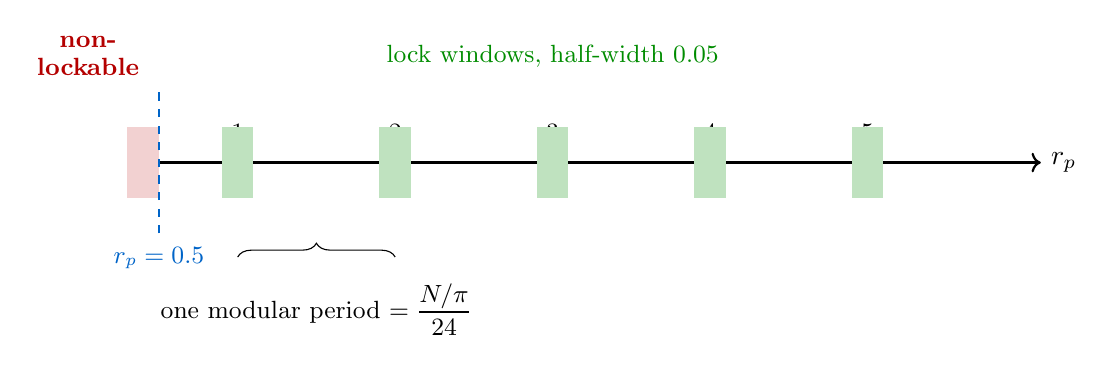
\begin{tikzpicture}[scale=1.0]
  \draw[->, thick] (-0.4,0) -- (11.2,0) node[right] {$r_p$};
  \foreach \x/\l in {1/1, 3/2, 5/3, 7/4, 9/5} {
    \draw[thick] (\x,-0.15) -- (\x,0.15) node[above] {\small \l};
    \fill[signalgreen!25] (\x-0.2,-0.45) rectangle (\x+0.2,0.45);
  }
  \fill[signalred!18] (-0.4,-0.45) rectangle (0,0.45);
  \draw[dashed, thick, floorblue] (0,-0.9) -- (0,0.9);
  \node[floorblue, below] at (0,-0.95) {\small $r_p = 0.5$};
  \node[signalred, align=center] at (-0.9,1.35) {\small\bfseries non-\\[-2pt]\small\bfseries lockable};
  \node[signalgreen] at (5,1.35) {\small lock windows, half-width $0.05$};
  \draw[decorate, decoration={brace, amplitude=5pt}] (1,-1.2) -- (3,-1.2)
        node[midway, below=6pt] {\small one modular period $=\dfrac{N/\pi}{24}$};
\end{tikzpicture}
\caption{The modular grid. A record locks when its position $r_p$ falls within $0.05$ of an
integer node. Because \texttt{nearest} is clamped to a minimum of $1$, every record with
$r_p < 0.5$ is compared against node $1$ and can never satisfy the tolerance. That boundary
sits at exactly half a modular period, at every register --- Equation~\ref{eq:floor}.}
\end{figure}

\section{Form C --- Preprocessing-Induced Concentration}

\begin{formbox}
\textbf{Form C.} Structure introduced by an operation applied to the lake before the pipeline
saw it. Invisible to all three nulls, because the nulls are generated after the operation and
do not replicate it.
\end{formbox}

The Gaia kinematic lake stores a sector-normalised scalar, formed by subtracting a per-sector
mean and adding the global mean. Three lakes in the survey carry
\texttt{sector\_normalized: true}: \texttt{s1\_gaia\_parallax},
\texttt{s2\_stellar\_kinematics}, and \texttt{g1\_galaxy\_kinematics}.

The below-floor mass of such a lake forms a coherent \emph{block} occupying exactly half a
modular period (Equation~\ref{eq:floor}). A per-sector shift does not disperse that block --- it
translates it, and where it lands relative to the node is determined entirely by
$\Delta_j \bmod \text{period}$.

\begin{figure}[H]
\centering
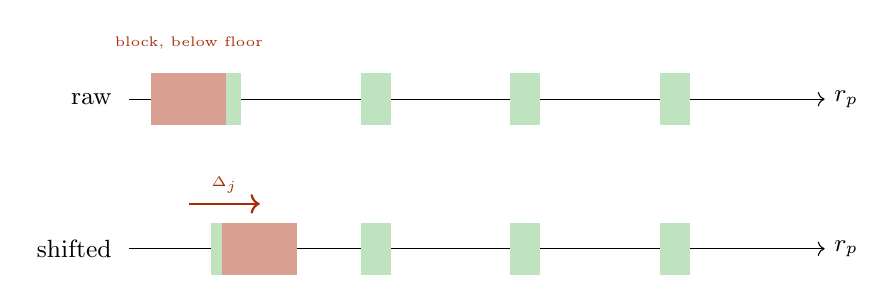
\begin{tikzpicture}[scale=0.95]
  \begin{scope}
    \draw[->] (-0.3,0) -- (9,0) node[right] {\small $r_p$};
    \foreach \x in {1,3,5,7} {\draw (\x,-0.12) -- (\x,0.12);
      \fill[signalgreen!25] (\x-0.2,-0.35) rectangle (\x+0.2,0.35);}
    \fill[cruciblered!45] (0,-0.35) rectangle (1,0.35);
    \node[left] at (-0.4,0) {\small raw};
    \node[cruciblered] at (0.5,0.75) {\tiny block, below floor};
  \end{scope}
  \begin{scope}[yshift=-2cm]
    \draw[->] (-0.3,0) -- (9,0) node[right] {\small $r_p$};
    \foreach \x in {1,3,5,7} {\draw (\x,-0.12) -- (\x,0.12);
      \fill[signalgreen!25] (\x-0.2,-0.35) rectangle (\x+0.2,0.35);}
    \fill[cruciblered!45] (0.95,-0.35) rectangle (1.95,0.35);
    \node[left] at (-0.4,0) {\small shifted};
    \draw[->, thick, cruciblered] (0.5,0.6) -- (1.45,0.6) node[midway, above] {\tiny $\Delta_j$};
  \end{scope}
\end{tikzpicture}
\caption{Form C. In raw form the half-period block sits below the floor and contributes no
locks. A per-sector additive shift translates the whole block; if it lands on a node, a
substantial fraction of the domain locks at once. Different sectors carry different offsets and
light different registers.}
\end{figure}

\begin{warningbox}
The decisive objection is not the mechanism but the null. The chaos null is generated by uniform
sampling over the empirical range of the \emph{normalised} scalars. It does not replicate the
per-sector shift. The comparison being made was normalised-real against unnormalised-uniform:
the null was blind to the single operation most capable of manufacturing the effect.

\medskip
\noindent This is disqualifying independently of whether any artifact mechanism is
demonstrated. A normalised scalar tested against an unnormalised null cannot support a lock
claim.
\end{warningbox}

Sector normalisation is defensible astrophysics --- Gaia has genuine sky-position-dependent
selection effects. The ruling is not that the operation is illegitimate. It is that if retained,
it must be re-pre-registered as its own domain, with a null that applies the identical
per-sector procedure to surrogate data.

\section{Form D --- Null-Support Mismatch}

\begin{formbox}
\textbf{Form D.} The null's lockable support does not match the data's. A uniform null over the
empirical range carries a small below-floor fraction; a right-skewed real distribution carries a
large one. The null is structurally more lockable than the data it scores, and the resulting $z$
measures that difference.
\end{formbox}

This is the form with the widest reach. It biased every negative verdict in eleven volumes.

\subsection{The Measurement}

Direct measurement of \texttt{s2\_stellar\_kinematics} against the floor:

\begin{table}[H]
\centering
\small
\begin{tabular}{@{}lrr@{}}
\toprule
& \textbf{below the $16/\pi$ floor} \\
\midrule
Real distribution (1{,}808{,}145 records) & \textbf{27.53\%} \\
Uniform chaos null over the same range & \textbf{2.50\%} \\
\bottomrule
\end{tabular}
\end{table}

\begin{figure}[H]
\centering
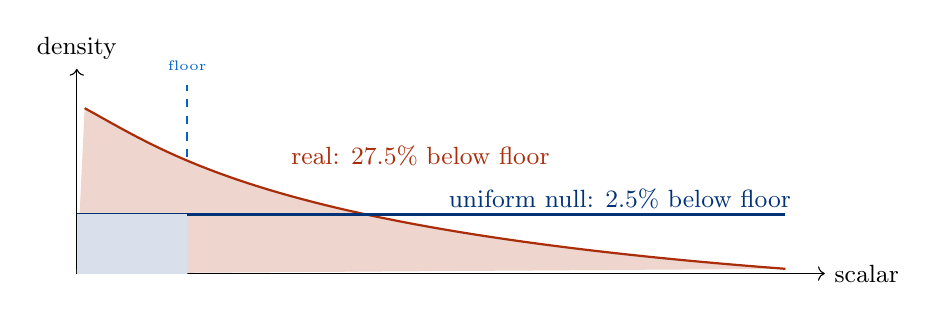
\begin{tikzpicture}[scale=1.0]
  \draw[->] (0,0) -- (9.5,0) node[right] {\small scalar};
  \draw[->] (0,0) -- (0,2.6) node[above] {\small density};
  \draw[dashed, thick, floorblue] (1.4,0) -- (1.4,2.4);
  \node[floorblue, above, align=center] at (1.4,2.45) {\tiny floor};
  \fill[cruciblered!20] (0,0) -- (0.1,2.1) .. controls (1.2,1.5) and (2.5,0.55) .. (9,0.06) -- (0,0);
  \draw[thick, cruciblered] (0.1,2.1) .. controls (1.2,1.5) and (2.5,0.55) .. (9,0.06);
  \draw[thick, kishblue] (0,0.75) -- (9,0.75);
  \fill[kishblue!15] (0,0) rectangle (1.4,0.75);
  \node[cruciblered, right] at (2.6,1.5) {\small real: 27.5\% below floor};
  \node[kishblue, right] at (4.6,0.95) {\small uniform null: 2.5\% below floor};
\end{tikzpicture}
\caption{Form D. Both arms span the same range, so the null appears fair. They place very
different amounts of mass in the mechanically non-lockable region, and the resulting $z$ is a
measurement of that difference rather than of harmonic structure.}
\end{figure}

\subsection{The Demonstration}

If the entire signal is floor mismatch, then predicting the lock rate from the below-floor
fraction alone --- assuming \emph{no harmonic structure whatsoever} --- should reproduce the
observed profile:

\begin{equation}
\widehat{\text{lock}}(N) \;=\; \bigl(1 - f_{\text{below}}(N)\bigr) \times 0.10 .
\label{eq:floormodel}
\end{equation}

\begin{signalbox}
Against the 23-register profile of \texttt{stellar\_kinematic}:

\medskip
\begin{tabular}{@{}lr@{}}
mean absolute error & \textbf{1.23\%} \\
maximum error & 2.67\% \\
$\operatorname{corr}\bigl(f_{\text{below}}(N),\ \text{observed lock rate}\bigr)$ & \textbf{$-0.99708$} \\
\end{tabular}

\medskip
\noindent Every register. No structure assumed. The monotonic decline in observed lock rate
from $0.0828$ at $4/\pi$ to $0.0669$ at $26/\pi$ tracks the monotonic rise in below-floor
fraction from 16.7\% to 32.5\%, because a higher register has a higher floor.
\end{signalbox}

\subsection{The Sign Bound}

Form D has a property that limits the damage, and it is worth proving rather than asserting.
The below-floor fraction is the domain's own cumulative distribution function evaluated at the
floor:

\begin{equation}
f_{\text{below}}(N) = F\!\left(\frac{N}{48\pi}\right).
\end{equation}

\noindent A CDF is non-decreasing, and $N/48\pi$ is increasing in $N$. Therefore
$f_{\text{below}}$ is monotonically increasing in $N$ for \emph{any} distribution.

\begin{signalbox}
A monotonic function has no local maxima. \textbf{Form D can produce a smooth negative baseline
deepening with $N$, but it cannot manufacture a peak at any register.}

\medskip
\noindent Consequently every positive claim in the survey was scored against a headwind, and
every \emph{negative} verdict --- ``noise floor'', ``anti-signal'' --- is in question.
\end{signalbox}

\subsection{The Residual}

Common support removes the clamp discontinuity. It does not remove the shape mismatch above the
floor: the real distribution remains skewed while the null remains uniform. On severity-matched
structureless data the residual after correction reaches $\lvert z\rvert \approx 10.6$, and
--- unlike Form D proper --- it is \emph{not} monotonic. It is an alignment-against-grid
quantity, which is the same kind of object a lock is, and can therefore carry local structure.

That is why the offset-sweep baseline of Chapter 3 is measured per register rather than per
domain. With it applied, the residual falls to a maximum of $3.52$.

\section{Form E --- Quantised Support}

\begin{formbox}
\textbf{Form E.} The domain takes a small number of distinct values. The lock statistic reduces
to whether those specific values land near nodes, and the record count inflates $z$ far beyond
the information content.
\end{formbox}

\subsection{The Tidal Domains}

\texttt{planetary\_atlantic} reports a lock rate of $0.5054$ at $17/\pi$ --- more than half the
lake. The domain carries \textbf{fifteen distinct scalar values}.

\begin{table}[H]
\centering
\small
\begin{tabular}{@{}lrrr@{}}
\toprule
\textbf{Domain} & \textbf{$n$} & \textbf{distinct} & \textbf{locked mass on top values} \\
\midrule
\texttt{planetary\_atlantic} & 6{,}973 & 15 & \textbf{99.7\% on 12.0000 h} \\
\texttt{planetary\_gulf} & 6{,}927 & 23 & 96.2\% on \{12.0000, 8.0000\} \\
\texttt{planetary\_pacific} & 6{,}838 & 22 & 90.6\% on 14.0000 h \\
\texttt{planetary\_indian} & 4{,}929 & 40 & 86.2\% on 14.0000 h $\pm$ 1 s \\
\bottomrule
\end{tabular}
\end{table}

\subsection{The Decisive Calculation}

The principal lunar semidiurnal constituent $M_2$ has a period of \textbf{12.4206 hours}, not
12. A lake reporting integer hours is reporting a rounded quantity. Testing both:

\begin{table}[H]
\centering
\small
\begin{tabular}{@{}lrrrl@{}}
\toprule
\textbf{Value} & \textbf{scalar} & \textbf{$r_p$ at $17/\pi$} & \textbf{distance to node} & \\
\midrule
$12.0000$ h (what the lake contains) & $1.575658$ & $6.9883$ & $0.0117$ & \textbf{locks} \\
$12.4206$ h (true $M_2$) & $1.595130$ & $7.0751$ & $0.0751$ & \textbf{does not lock} \\
\bottomrule
\end{tabular}
\end{table}

\begin{figure}[H]
\centering
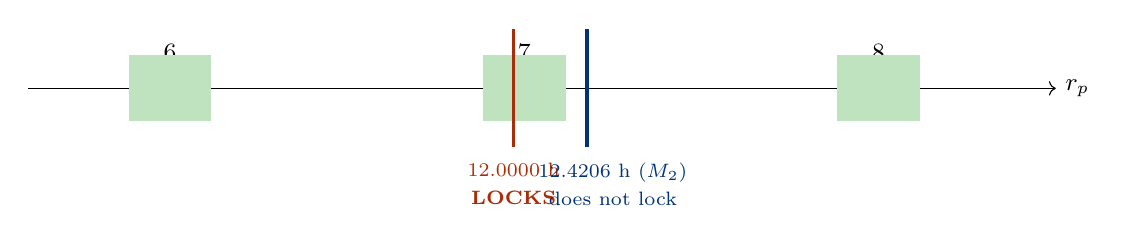
\begin{tikzpicture}[scale=1.5]
  \draw[->] (-0.2,0) -- (8.5,0) node[right] {\small $r_p$};
  \foreach \x/\l in {1/6, 4/7, 7/8} {
    \draw[thick] (\x,-0.1) -- (\x,0.1) node[above=2pt] {\small \l};
    \fill[signalgreen!25] (\x-0.35,-0.28) rectangle (\x+0.35,0.28);
  }
  \draw[very thick, cruciblered] (3.91,-0.5) -- (3.91,0.5);
  \node[cruciblered, below, align=center] at (3.91,-0.55) {\scriptsize 12.0000 h\\[-2pt]\scriptsize \textbf{LOCKS}};
  \draw[very thick, kishblue] (4.53,-0.5) -- (4.53,0.5);
  \node[kishblue, below, align=center] at (4.75,-0.55) {\scriptsize 12.4206 h ($M_2$)\\[-2pt]\scriptsize does not lock};
\end{tikzpicture}
\caption{Form E made concrete. Two tick marks 0.42 hours apart at $17/\pi$. The rounded integer
falls inside the lock window; the physical semidiurnal period falls outside it. A
\textsc{strong} classification on 3{,}515 records hangs on which of the two the lake recorded.}
\end{figure}

\subsection{The Arithmetic of the Modulus Itself}

\texttt{orbital\_ttv} --- transit timing variation, $n = 290{,}458$, reported \textsc{strong} at
$16/\pi$ --- carries its top five locked values at raw $1, 3, 7, 15, 31$ minutes. Those are
$2^m - 1$, and their scalars are exact integer multiples of $\ln 2 / \ln \kgeo = 0.425803$.

For such values,
\begin{equation}
r_p \;=\; m \cdot \frac{24\pi \ln 2}{N \ln \kgeo} \;=\; m \cdot \frac{32.1048}{N},
\end{equation}
\noindent and $32.1048$ lies $0.32$ percent from $32 = 2^5$. The ratio is therefore near-integer
at $N = 4$, $8$, $16$ --- the powers of two dividing 32 --- and nowhere else in the family.

\begin{table}[H]
\centering
\small
\begin{tabular}{@{}rrrl@{}}
\toprule
$N$ & $32.1048/N$ & \textbf{multiples of $2^m-1$ that lock} & \textbf{observed $\Delta$} \\
\midrule
16 & $2.0065$ & $m = 1\ldots7$ (seven) & $+0.0473$ \\
8 & $4.0131$ & $m = 1,2,3$ (three) & $+0.0351$ \\
4 & $8.0262$ & $m = 1$ (one) & $-0.0194$ \\
\bottomrule
\end{tabular}
\caption{The per-multiple error accumulates with $m$, so the higher register retains more
multiples. The observed ordering is exactly the count of surviving multiples.}
\end{table}

Modelling \texttt{orbital\_ttv} as \emph{nothing but integer minutes} with a $1/x$ weight, and
assuming no harmonic structure at all, reproduces the observed profile at a correlation of
$+0.804$, with the same peak register and four of the top five.

\begin{warningbox}
\textbf{This is a property of the modulus, not of the data.} Any binary-commensurate
quantisation, in any domain, will favour registers 4, 8 and 16. The framework's principal
register is the one most vulnerable to this artifact.

\medskip
\noindent It does not make $16/\pi$ results wrong. It means the evidential burden on a $16/\pi$
claim is higher than on any other register, and that continuous-support verification is
mandatory before any $16/\pi$ classification. A continuous domain has no quantisation grid and
cannot be reached by this mechanism. \texttt{quantum\_transitional} carries more than 50{,}000
distinct values and is unreachable.
\end{warningbox}

The screen generalises beyond base two: a grid of spacing $g$ produces preferred registers
wherever $24\pi \ln g / (N \ln \kgeo)$ is near-integer. For decimal rounding, $g = 10$ gives a
constant of $106.65$, favouring registers near 4 and 5. Round-number decimal quantisation is far
more common in promoted data than binary.

\section{The Screens Now Standing}

\begin{table}[H]
\centering
\small
\begin{tabular}{@{}lp{0.62\textwidth}@{}}
\toprule
\textbf{Screen} & \textbf{Catches} \\
\midrule
Dispatch attribution & Form C at source: a domain reading a precomputed scalar rather than its configured field \\
Common support + baseline & Form D and its residual \\
Kept-fraction per register & Under-resolved domains; out-of-range reporting \\
Periods-spanned & Domains with too few nodes across their entire range \\
Distinct-value / grid screen & Form E, including grids other than base two \\
Node-occupancy histogram & Form C and E: locked mass concentrated on one or few node indices \\
Look-elsewhere correction & Trials-factor inflation across 1{,}150 register-domain tests \\
\bottomrule
\end{tabular}
\caption{Every screen is run on every domain on every run, and its result published.}
\end{table}

% ==============================================================================
\chapter{The Crucible: Lake by Lake}
% ==============================================================================

\section{What the Fire Showed}

The forms of Chapter 4 are mechanisms. This chapter is what they did to specific lakes. Each
entry states what was found, how it was found, and what the lake now requires.

\subsection{\texttt{s2\_stellar\_kinematics} --- 27.5\% Non-Measurements}

The Gaia transverse velocity lake carries 1{,}808{,}145 records. Measured against the $16/\pi$
floor of $0.188535$~km/s:

\begin{itemize}
    \item \textbf{497{,}831 records (27.53\%)} sit at or below it.
    \item 125{,}726 records (6.95\%) carry $v_T < 0.005$~km/s.
    \item The minimum is $4.88 \times 10^{-13}$~km/s.
\end{itemize}

For a stellar population with velocity dispersion $\sigma \approx 30$~km/s, the expected
fraction below $0.19$~km/s is approximately $2 \times 10^{-5}$ --- about $0.002$ percent. The
lake contains $27.53$ percent. That is four orders of magnitude, not a tail effect.

\begin{nullbox}
A transverse velocity of $10^{-13}$~km/s is not a measurement. These are almost certainly
proper motions at or beneath Gaia's detection floor, promoted without filtering. The identical
minimum appears in \texttt{s2\_wrongbox}, confirming a shared source.
\end{nullbox}

\textbf{Required:} a physical validity criterion, pre-registered --- proper motion above a fixed
multiple of its own quoted Gaia uncertainty. Not a threshold chosen at the scalar level after
its effect is known. If \texttt{pmra\_error} and \texttt{pmdec\_error} are absent from the
promoted lake, that is a promotion defect and the lake rebuilds from source.

\textbf{Note:} the filter does not fix Form D. Removing the visibly absurd 6.95\% still leaves
roughly 20\% below floor. These are two separate defects that happen to overlap in this lake.

\subsection{The Tidal Lakes --- Rounded to Integer Hours}

Covered in Chapter 4. \textbf{Required:} rebuild from NOAA CO-OPS timestamps at native
precision. The precision exists upstream --- \texttt{t2\_planetary}'s raw payload records times
to the minute (\texttt{04:59} to \texttt{09:40}, giving $4.683333$ hours). If the lock survives
at native precision it is real; if it vanishes, Form E is confirmed. Suspension, not withdrawal,
pending that run.

\subsection{\texttt{orbital\_ttv} --- Whole Minutes}

Same remedy, same falsification structure. Suspended pending a native-precision rebuild.

We record one honest residual: the quantisation model under-predicts the observed peak at
$17/\pi$, where the locking multiples are $m = 9$ and $m = 18$, both low-weight. Something at
$17/\pi$ is not explained by quantisation. That is precisely what a native-precision re-run
would resolve, and it is stated here rather than smoothed over by the correlation coefficient.

\subsection{\texttt{stellar\_spindown} --- Eleven Orders of Magnitude Annihilated}

Pulsar spin-down rates span $1.17\times10^{-21}$ to $5.49\times10^{-10}$~s/s. Because
$\ln(1+x) \approx x$ for $x \ll 1$, and $x_0 = 1.0$, the entire domain maps to scalars of order
$10^{-10}$ --- nine orders of magnitude beneath the lock floor of $0.106$.

The domain carries \textbf{zero information}. It cannot have been an honest null in any volume
in which it appeared, because there was nothing to null.

This is the same scale annihilation that disqualified two wrongboxes (below), occurring in a
domain treated as real data. Its root is broader than one lake: \textbf{$x_0 = 1.0$ is set for
all domains}, regardless of the natural scale of the quantity. The parameter exists to fix the
reference scale and has never been used.

\subsection{\texttt{n4\_cosmological} --- A Null That Reproduces Its Own Domain}

\texttt{t4\_cosmological} carries \texttt{d\_proxy}, a Hubble distance $cz/H_0$ in Mpc, over a
redshift range of $z \in [0.01000, 0.01596]$ --- implying a scalar range of
$[2.32224, 2.60416]$.

\texttt{n4\_cosmological}, the \emph{designated null} for that domain, carries a measured scalar
range of $[2.32227, 2.60422]$.

\begin{erratumbox}
Agreement to $3\times10^{-5}$ and $6\times10^{-5}$. The null for the cosmology domain has the
same scalar distribution as the cosmology data.

\medskip
\noindent Both lock at $15/\pi$: \texttt{cosmology} at $+18.7$ and \texttt{null\_cosmology\_null}
at $+11.3$. The null locked because the null \emph{is} the signal. Every statement of the form
``the null did not lock'' that rests on this lake is void.
\end{erratumbox}

\textbf{Required:} rebuild or withdraw before either domain enters any test.

\subsection{\texttt{t4\_cosmological} --- Under-Resolved}

The same measurement exposed a second problem. That scalar range spans $0.282$ units. At
$15/\pi$ the modular period is $0.19894$, so the entire domain spans \textbf{1.42 modular
periods}. It locks at $15/\pi$ with roughly one and a half nodes available across its whole
range.

That places it with \texttt{orbital\_eccentricity} (1.93 periods) and \texttt{galactic\_sersic}
(2.01 periods). A register identification on two nodes is not a distributional finding.

\subsection{\texttt{chemistry} --- Not a Broken Lake}

Reported early in the audit as requiring a rebuild, on the evidence that \texttt{scalar\_klc}
and \texttt{\_raw\_payload.scalar\_invariant} were bit-identical, implying no log transform was
applied.

The lake is intact. The named handler \texttt{scalarize\_chemistry} returns the stored invariant
verbatim, by construction. The passthrough is in the engine, not the data. Recorded here because
a rebuild was nearly ordered on a misdiagnosis.

\section{The Wrongbox Tier}

A wrongbox applies deliberately \emph{wrong} mathematics to \emph{right} data, and is expected
not to lock. The tier was believed to comprise four working controls.

\begin{table}[H]
\centering
\small
\begin{tabular}{@{}lrl@{}}
\toprule
\textbf{Wrongbox} & \textbf{below-floor mass} & \textbf{Verdict} \\
\midrule
\texttt{stellar\_wrongbox} & 87.7\% $\to$ 99.6\% & scale annihilation, not projection wrongness \\
\texttt{kinematic\_wrongbox} & $\approx$ 38--42\% & same \\
\texttt{orbital\_wrongbox} & $\approx$ 3\% & \textbf{genuine control} \\
\texttt{materials\_wrongbox} & $\approx$ 1\% & \textbf{genuine control} \\
\bottomrule
\end{tabular}
\end{table}

\begin{rulingbox}
\textbf{Rule 1.5, second clause.} A wrongbox is a valid control only when its wrong projection
does not shrink the scalar below the lock floor. \texttt{log\_inverse} of a large quantity and
\texttt{log\_volumetric} of a sub-unit quantity are \emph{scale annihilators}, not wrong
projections. The retained fraction under common support must be published for every wrongbox,
and any wrongbox retaining less than a pre-registered fraction is reported \textsc{out-of-range},
never \textsc{collapse}.
\end{rulingbox}

The direct evidence is stark. In the canonical run, \texttt{stellar\_spindown} $\times$
\texttt{stellar\_wrongbox} produced the \textbf{third-highest cross-domain pinch in the entire
table}. \texttt{stellar\_spindown} carries no information; \texttt{stellar\_wrongbox} is 99.6\%
below floor. Two informationless domains, agreeing at rank three.

\texttt{orbital\_wrongbox} is the template: cubed orbital periods spanning six orders of
magnitude, never approaching the floor, returning real $\approx 0.098$ against chaos
$\approx 0.098$, $\Delta \approx 0$. That is a wrongbox doing its job, and it is the only clean
demonstration in the tier.

\section{The New Lake Boundaries}

The following become standing promotion requirements. No lake is admitted without them.

\begin{enumerate}
    \item \textbf{Native precision.} A lake states the precision of its source and promotes at
          it. Rounding is a promotion decision and must be declared, not inherited.
    \item \textbf{Declared physical plausibility range.} Every lake states the expected range of
          its quantity from independent physics, and the fraction of records outside it, before
          admission. The distributional litmus test cannot see physical implausibility: a lake
          roughly a quarter composed of non-measurements passed it.
    \item \textbf{Measured object overlap.} Where two lakes may describe the same objects, the
          overlap is \emph{measured}, not assumed. Where partial, the intersecting records are
          removed from one pre-registered side rather than a domain being discarded.
    \item \textbf{Declared $x_0$.} The reference scale is drawn from independent physics, cited,
          and filed before the run --- never adjusted after a register is seen.
    \item \textbf{Periods spanned, published.} Any domain below the pre-registered minimum is
          reported as insufficient-resolution rather than given a register.
    \item \textbf{Distinct-value count and grid detection, published.}
\end{enumerate}

\subsection{A Worked Example of Requirement 3}

\texttt{t4\_cosmological} (SDSS DR16 redshift) and \texttt{g1\_galaxy\_kinematics} (SDSS DR16
velocity dispersions) were candidates to be collapsed into a single family on the suspicion of
shared objects. Rather than assume, the overlap was matched on sky position at 1-arcsecond
tolerance:

\begin{table}[H]
\centering
\small
\begin{tabular}{@{}lr@{}}
\toprule
matched pairs & 971 \\
fraction of \texttt{t4\_cosmological} & 19.42\% \\
fraction of \texttt{g1\_galaxy\_kinematics} & 0.053\% \\
redshift range overlap & 100\% of A, 0.6\% of B \\
\bottomrule
\end{tabular}
\end{table}

Partial, not fatal. The 971 intersecting records are removed from \texttt{t4\_cosmological} and
both domains are retained as independent families. Collapsing an entire domain on a suspicion
would have discarded a lake over a fifth of a small sample.

We note the caveat the measurement also surfaced: zero object overlap would not have implied
independence. Two disjoint samples drawn from the same flux-limited survey over the same
redshift range are correlated through selection.

% ==============================================================================
\chapter{The Controlled Same-Object Experiment}
% ==============================================================================

\section{A Liability Turned Into a Prediction}

Volume 11 reported multi-attribute measurement of a single population as a strength. Volume 12
must correct that: measuring one population several ways produces results correlated
\emph{by construction}. Stellar colour against stellar luminosity is the Hertzsprung--Russell
relation, known since 1911. Galaxy dispersion against galaxy mass is Faber--Jackson. The two
muon momenta come from the same event kinematics.

Such pairs cannot be counted as independent corroboration. But the information in them is real,
and there is a way to extract it that turns the correlation from a liability into a test.

\begin{signalbox}
\textbf{Where the physical relation between two attributes is known, the framework makes a
falsifiable prediction about the \emph{register pair}.}
\end{signalbox}

\section{The Kepler Case}

Kepler's third law gives $a^3 \propto P^2$, hence

\begin{equation}
s_a \;=\; \tfrac{2}{3}\, s_P \;+\; c, \qquad c = \frac{\ln(\text{const})}{\ln \kgeo},
\end{equation}

\noindent a deterministic affine map in scalar space. A record locked at register $N$ in period
satisfies $s_P = n N/(24\pi)$ for integer $n$. Its radius scalar is then

\begin{equation}
r_p^{(a)} \;=\; \frac{2}{3}\cdot\frac{nN}{M} \;+\; \frac{24\pi c}{M},
\end{equation}

\noindent which is integer for all $n$ when $M = \tfrac{2}{3}N$ and the constant term is itself
a whole number of periods.

\begin{table}[H]
\centering
\small
\begin{tabular}{@{}lc@{}}
\toprule
\textbf{Period register $N$} & \textbf{Predicted radius register $M = \tfrac{2}{3}N$} \\
\midrule
6, 9, 12, 15, 18, 21, 24 & 4, 6, 8, 10, 12, 14, 16 \\
all others & non-integer --- \textbf{no coherent lock predicted} \\
\bottomrule
\end{tabular}
\caption{The framework's prediction for the orbital period/radius pair. The prediction is
determined entirely by Kepler and the modulus; nothing is fitted.}
\end{table}

\begin{predictionbox}
\textbf{Observed:} \texttt{orbital} (period) locks at $22/\pi$. Since $\tfrac{2}{3}\times 22 =
14.67$ is not an integer register, the framework predicts that \texttt{orbital\_radius} should
\emph{not} lock coherently at any register.

\medskip
\noindent \textbf{Observed:} \texttt{orbital\_radius} does not lock.
\end{predictionbox}

This is a same-object pair used as a \emph{control} rather than as corroboration. The physical
relation is known, so the register relation is predicted, and the pair is capable of falsifying
the framework instead of flattering it.

\section{The Controlled-Pair Programme}

Three further pairs carry exact or near-exact physical relations and are pre-registered in
Chapter 9 for the next canonical run:

\begin{itemize}
    \item \textbf{Pulsar characteristic age.} $\tau = P/2\dot{P}$ is exact, relating
          \texttt{stellar\_rotation\_pulsar}, \texttt{stellar\_spindown} and
          \texttt{stellar\_age}. A three-way closure test, once $x_0$ is set so that spin-down
          rate is not annihilated.
    \item \textbf{Faber--Jackson.} $L \propto \sigma^4$, relating \texttt{galactic} and
          \texttt{galactic\_mass}. Approximate rather than exact, so the prediction is a
          register \emph{band} rather than a point.
    \item \textbf{Dimuon kinematic closure.} Invariant mass is a known function of the two
          transverse momenta and the pseudorapidities, relating four CMS domains.
\end{itemize}

\begin{warningbox}
The controlled-pair design requires the lakes to be built for it. A pair drawn opportunistically
from lakes promoted for other purposes inherits whatever promotion artifacts each carries
independently. The pairs above must be promoted \emph{as pairs}, from a common object list, at
a common precision, with the physical relation stated and the register prediction filed before
the run.
\end{warningbox}

% ==============================================================================
\chapter{Errata}
% ==============================================================================

\section{On the Purpose of This Chapter}

This programme publishes its missteps. A volume that records only confirmations has told the
reader nothing about its error rate, and a method whose failures are invisible cannot be
evaluated.

The errata below include corrections that went against the referee and against the architect.
Both are recorded, because an errata culture that only documents other people's errors is not
one.

\section{Erratum 1 (Volume 11) --- Re-Confirmed and Extended}

\begin{erratumbox}
\textbf{Original finding (Vol 11):} the scramble null is inert for the per-value lock test.
The lock statistic is computed over the multiset of scalars and is order-independent;
\texttt{random.shuffle} cannot change an order-independent statistic. Scoring the scramble null
through the lock mathematics returns the real $z$ identically --- not approximately, identically.

\medskip
\textbf{Independent re-confirmation (Vol 12):} demonstrated on 20{,}000 synthetic scalars. Real
and scramble lock rates are bit-identical at $12/\pi$, $16/\pi$ and $20/\pi$.

\medskip
\textbf{New extension (Vol 12):} Erratum 1 assigned the scramble a \emph{surviving} role as a
control for record-ordering and cross-domain pairing artifacts. The engine never implemented
that role. \texttt{build\_pinch\_table.py} defines loaders for the chaos and synthetic nulls
only; a search for ``scramble'' across the pinch, figure, unify and pipeline code returns
nothing. The files are written to disk and discarded.
\end{erratumbox}

\begin{correctionbox}
The Volume 12 audit initially reported the scramble finding as new. It was not. The material was
already published, dated, in Volume 11's own errata section, and the architect filed it without
searching the record.

\medskip
\noindent \textbf{Standing rule adopted:} the errata register is searched, and the result cited,
before any engine or methods finding is filed. A finding enters a ruling request with a
line-and-file citation to prior work, or with an explicit statement that the record was searched
and is silent.
\end{correctionbox}

\textbf{Scope limit, stated precisely.} The ARPES $24/\pi$ and Fermi $20/\pi$ artifacts were
caught by \emph{dedicated scramble control lakes} --- separately promoted files that ran through
the whole pipeline as independent domains. That mechanism worked and is unaffected. Only claims
resting on the engine's internal tier require re-checking. Phoenix's language sweep of Volumes
9--11 distinguishes the two.

\section{Erratum 2 (Volume 11) --- Carried Forward}

The chaos null is uniform-range rather than value-shuffle. Recorded in Volume 11 and unchanged.
Its consequence is developed as Form D in Chapter 4: a uniform null over the empirical range
does not reproduce a skewed distribution's below-floor mass.

\section{Erratum 3 --- The Lock Floor and the Orbital Demonstration}

\begin{erratumbox}
The lock floor is an algebraic identity: $s_{\text{floor}}(N) = (N/\pi)/48$, exactly half a
modular period at every register. Expressed in raw units this is $0.1885$ at $16/\pi$, applied
identically whatever the unit.

\medskip
Volume 11 published: \emph{``Kepler orbital periods lock (\textsc{strong} at $16/\pi$), orbital
radii do not (noise floor throughout). Same 13{,}000 planets. Different geometric question.
Different result.''}

\medskip
P1 is measured in days (typical range 1--500), P2 in AU (typical 0.02--1), P3 in Jupiter masses
(typical 0.003--2). The majority of P2 and P3 records sit below the floor and were mechanically
barred from locking. \textbf{The published contrast may reflect unit magnitude rather than
geometry.}
\end{erratumbox}

\textbf{Scope, stated neither wider nor narrower.} The stellar four-panel demonstration is
unaffected on this count: \texttt{s1\_gaia\_parallax} sits at $r_p = 17.9$, far above the floor,
so its behaviour is a genuine measurement. Only the orbital demonstration requires
re-derivation.

\begin{signalbox}
\textbf{A null from a domain below the lock floor is not evidence of absence.} Such domains are
reported \textsc{out-of-range}, with the floor value and the retained fraction stated, and are
excluded from \textsc{strong}/null tables entirely.
\end{signalbox}

\section{Erratum 4 --- The Principal Erratum of This Volume}

\subsection{4a. \texttt{stellar\_kinematic} Withdrawn}

\begin{erratumbox}
Volume 11 reported \texttt{stellar\_kinematic}, $n = 1{,}808{,}145$, at $15/\pi$ with
$Z = +98.3$ and $16/\pi$ at $+94.0$.

\medskip
Computed from raw transverse velocity rather than from the sector-normalised precomputed
scalar, the domain returns negative $z$ at all twenty-three registers. Under the corrected
statistic of Chapter 3 it returns a flat profile spanning $-0.7$ to $-5.3$ --- an honest null.

\medskip
\textbf{The $15/\pi$--$16/\pi$ stellar band is withdrawn.}
\end{erratumbox}

The reasoning is given in Chapter 4 (Form C). The decisive point is not the artifact mechanism
but the null: a normalised scalar tested against an unnormalised null cannot support a lock
claim, whatever the normalisation does.

\textbf{Controls.} Three lakes carry sector normalisation. \texttt{g1\_galaxy\_kinematics}
resolved its field in \texttt{\_raw\_payload} even under the Volume 11 lookup, never entered the
fallback, was always computed from raw, and is unchanged. \texttt{s1\_gaia\_parallax} moved from
normalised to raw with no material change. Only \texttt{s2} moved. That asymmetry is recorded
and is not explained.

\subsection{4b. Form D and the Standing of Every Negative Verdict}

Developed in Chapter 4. Every ``noise floor'', ``anti-signal'' and ``collapse'' classification
in Volumes 5--11 was scored against a null structurally more lockable than the data. Positive
claims are unaffected --- Form D is monotonic in $N$ and cannot manufacture a peak --- but the
negative half of the ledger is in question and is being regenerated.

\subsection{4c. The Wrongbox Tier}

Two of four controls demonstrated scale annihilation rather than projection wrongness.
Every statement of the form ``the wrongbox collapsed as designed'' in Volumes 5--11 is restated,
distinguishing the two that demonstrated wrongness from the two that demonstrated annihilation.

\subsection{4d. Form E and the Suspended Domains}

The four tidal domains, \texttt{orbital\_ttv} and \texttt{stellar\_cycle} are \textbf{suspended},
not withdrawn, pending native-precision rebuild.

\subsection{4e. Volume 11's Internal Contradiction}

\begin{erratumbox}
Volume 11's pinch table reports \texttt{stellar} ($n = 2{,}000{,}000$) at $24/\pi$, $Z = +22.1$,
\textsc{strong}. Volume 9 carries the same domain at $24/\pi$, $Z = +20.68$.

\medskip
Volume 11's narrative, describing the \texttt{principle\_stellar\_proof} panels, states:
\emph{``Parallax distance (positional): Noise floor across all registers. No signal. The
positional measurement does not lock.''}

\medskip
The table and the narrative disagree about the same lake in the same volume. The
domain-to-lake mapping is unambiguous --- exactly one lake, \texttt{s1\_gaia\_parallax}, carries
the domain \texttt{stellar}, and $n$ matches exactly.

\medskip
The four-panel kinematic principle argument required parallax to be the panel that does
\emph{not} lock. Its own table says it locks. Combined with 4a, that figure loses both its
positive and its negative control. \textbf{It is withdrawn pending rebuild, not patched.}
\end{erratumbox}

\begin{correctionbox}
The architect initially reported this as \texttt{s1} having \emph{inverted} from a published
null to a lock under the corrected engine, and offered Volume 8 lake metadata as corroboration.
That was wrong. The claim was sourced from Volume 11's narrative without checking Volume 11's
own table. \texttt{s1} did not invert; it was always $24/\pi$. The corrected finding --- an
internal contradiction in the published volume --- is narrower and better evidenced.
\end{correctionbox}

\subsection{4f. Unit-Contingency of the Bridge Programme}

\begin{erratumbox}
For $x \gg x_0$, the scalarization reduces to
$\ln(x)/\ln \kgeo - \ln(x_0)/\ln \kgeo$. \textbf{A change of unit is an additive shift in scalar
space} --- the same operation as the sector normalisation of 4a --- and the lock test is
modular.

\medskip
Bridge 1 asserts that nuclear binding energy and galactic velocity dispersion share $21/\pi$.
Binding energy is expressed in MeV. In eV the shift is $\ln(10^6)/\ln(16/\pi) = 8.4869$ scalar
units against a $21/\pi$ period of $0.278521$: \textbf{30.47 periods, a phase change of 0.47 ---
the maximum possible displacement.}

\medskip
Every cross-domain register agreement in the Rosetta Atlas depends on unit choices that were
never pre-registered.
\end{erratumbox}

There is no phase-neutral $x_0$. A shift of $\Delta s$ moves phase by $\Delta s \cdot 24\pi/N$
periods, and that quantity is $N$-dependent; neutrality across the whole family would require a
value of order $5\times10^{10}$. \textbf{Any $x_0$ other than the current one changes register
assignment, and differently at different registers.} $x_0$ cannot be adopted as a correction to
a defective scalarization; it can only be adopted as an explicit component of a pre-registered
hypothesis --- \emph{quantity $Q$, expressed in reference unit $U$, locks at register $N$}. That
is a weaker claim than this programme has been making, and it is stated here in those words.

The test that decides it is pre-registered in Chapter 9.

\section{Erratum 5 --- The Cosmology Null}

\begin{erratumbox}
\texttt{n4\_cosmological}, the designated sovereign null for the cosmology domain, carries a
measured scalar range of $[2.32227, 2.60422]$. \texttt{t4\_cosmological}, the real domain,
implies $[2.32224, 2.60416]$ from its redshift range and Hubble distance proxy.

\medskip
Agreement to $3 \times 10^{-5}$. Both lock at $15/\pi$. \textbf{The null reproduces the domain
it was built to null.} Every statement resting on this null is void until it is rebuilt.
\end{erratumbox}

\section{Corrections Against the Referee}

Recorded in the same register as the others.

\begin{correctionbox}
\textbf{The spike hypothesis.} The referee proposed that Form C acted on a concentrated feature
--- a mass of records at a single scalar value --- inferred from a reported minimum of
\texttt{0.0000}. Direct measurement found no such pile: zero records at exactly zero, a minimum
of $4.88\times10^{-13}$, and smooth monotonic bin decay. The mechanism was replaced by the
half-period \emph{block}, which is the better object and which the referee accepted.

\medskip
\textbf{The sign bound.} The referee's monotonicity argument for Form D is correct and is proved
in Chapter 4. The architect extended it to the post-correction residual. The referee's disproof
used the architect's own table: the residual is not monotonic, exhibits a local maximum at
$15/\pi$ some eleven standard deviations from its neighbours, and is an alignment-against-grid
quantity --- the same kind of object a lock is. The extension was withdrawn and the per-register
baseline adopted in its place.
\end{correctionbox}

\noindent Three wrong hypotheses in this volume produced three real findings. The mechanism
being wrong is, in each case, what produced the more valuable result.

% ==============================================================================
\chapter{What the Nine Tell Us, and What They Do Not}
% ==============================================================================

\section{The Reduction}

\begin{table}[H]
\centering
\small
\begin{tabular}{@{}lrl@{}}
\toprule
\textbf{Stage} & \textbf{\textsc{strong}} & \textbf{What removed the difference} \\
\midrule
Run of 23 Aug, Vol 11.1 statistic, threshold $3.0$ & 28 & --- \\
Run of 26 Aug, corrected statistic, threshold $5.0$ & 21 & common support, baseline, threshold \\
After form and category screens & \textbf{9} & Form E (8), a null, a wrongbox, tiny-$n$ (2) \\
\bottomrule
\end{tabular}
\end{table}

Of the twelve removed at the last stage, \textbf{eleven} fell to form work or category. The
look-elsewhere gate removed exactly one: \texttt{cmb\_anisotropy} at $+6.0$ against a threshold
of $6.22$.

That distribution matters. The gate is not doing the reducing --- the crucible is. A threshold
that removed most of the ledger would suggest it had been set where the results were.

\section{The Nine}

\begin{table}[H]
\centering
\small
\begin{tabular}{@{}lrrrr@{}}
\toprule
\textbf{Domain} & \textbf{$n$} & \textbf{Register} & \textbf{$z_{\text{signal}}$} & \textbf{kept} \\
\midrule
\texttt{subnuclear\_mass} & 100{,}000 & $13/\pi$ & $+63.4$ & 100\% \\
\texttt{stellar\_colour} & 1{,}979{,}697 & $15/\pi$ & $+44.1$ & 100\% \\
\texttt{galactic} & 1{,}843{,}110 & $18/\pi$ & $+42.6$ & 100\% \\
\texttt{orbital} & 13{,}521 & $22/\pi$ & $+34.3$ & 100\% \\
\texttt{quantum\_transitional} & 189{,}330 & $16/\pi$ & $+31.2$ & \textbf{100\%} \\
\texttt{subnuclear\_pt\_sublead} & 100{,}000 & $26/\pi$ & $+24.5$ & 100\% \\
\texttt{subnuclear\_pt\_lead} & 100{,}000 & $26/\pi$ & $+19.7$ & 100\% \\
\texttt{cosmology} & 5{,}000 & $15/\pi$ & $+18.7$ & 100\% \\
\texttt{galactic\_mass} & 1{,}843{,}110 & $19/\pi$ & $+11.2$ & 100\% \\
\bottomrule
\end{tabular}
\caption{The corrected portrait. All nine clear the look-elsewhere threshold of $6.22$, the
weakest with a margin of $+4.98$.}
\end{table}

\subsection{Reproducibility}

Two independent runs of the pinch stage on identical input, at an identical engine fingerprint,
with the unseeded chaos null redrawn:

\begin{table}[H]
\centering
\small
\begin{tabular}{@{}lrrl@{}}
\toprule
\textbf{Domain} & \textbf{Run A} & \textbf{Run B} & \\
\midrule
\texttt{quantum\_transitional} & $16/\pi$ $+34.7$ & $16/\pi$ $+31.2$ & register stable \\
\texttt{galactic} & $18/\pi$ $+38.8$ & $18/\pi$ $+42.6$ & register stable \\
\texttt{stellar\_colour} & $15/\pi$ $+41.2$ & $15/\pi$ $+44.1$ & register stable \\
\texttt{orbital} & $22/\pi$ $+32.0$ & $22/\pi$ $+34.3$ & register stable \\
\texttt{stellar\_kinematic} & $12/\pi$ $-0.7$ & $12/\pi$ $-0.8$ & register stable \\
\bottomrule
\end{tabular}
\caption{Magnitudes jitter as Equation~\ref{eq:sdz} predicts. \textbf{Every register assignment
is identical.}}
\end{table}

\section{The Family Collapse}

\begin{warningbox}
Nine domains are not nine independent measurements. Same-object multi-attribute lakes are
correlated by construction, and the strongest cases are deterministic: \texttt{orbital} and
\texttt{orbital\_radius} are related by Kepler's third law, which makes one a closed-form
transformation of the other.
\end{warningbox}

Collapsing to independent families and taking the highest-$z$ representative of each:

\begin{figure}[H]
\centering
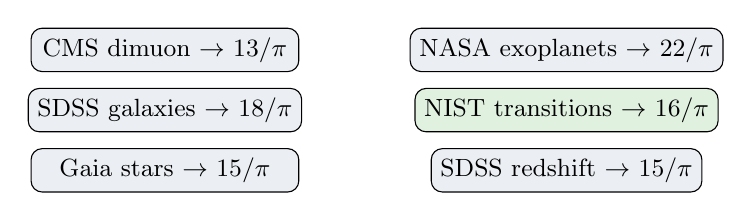
\begin{tikzpicture}[node distance=2mm, every node/.style={font=\small}]
  \node[draw, rounded corners, fill=kishblue!8, minimum width=3.4cm] (a) {CMS dimuon $\to$ $13/\pi$};
  \node[draw, rounded corners, fill=kishblue!8, minimum width=3.4cm, below=of a] (b) {SDSS galaxies $\to$ $18/\pi$};
  \node[draw, rounded corners, fill=kishblue!8, minimum width=3.4cm, below=of b] (c) {Gaia stars $\to$ $15/\pi$};
  \node[draw, rounded corners, fill=kishblue!8, minimum width=3.4cm, right=1.4cm of a] (d) {NASA exoplanets $\to$ $22/\pi$};
  \node[draw, rounded corners, fill=signalgreen!12, minimum width=3.4cm, below=of d] (e) {NIST transitions $\to$ $16/\pi$};
  \node[draw, rounded corners, fill=kishblue!8, minimum width=3.4cm, below=of e] (f) {SDSS redshift $\to$ $15/\pi$};
\end{tikzpicture}
\caption{Nine domains, six independent families. Registers $\{13, 15, 15, 16, 18, 22\}$ --- one
coincidence.}
\end{figure}

\begin{signalbox}
The probability of at least one repeated register among six independent draws from
twenty-three is
\[
1 - \prod_{i=0}^{5}\frac{23-i}{23} \;=\; \mathbf{0.509}.
\]
\textbf{A single shared register at this family count is more likely than not by chance.}
\end{signalbox}

\begin{warningbox}
\textbf{The nine are therefore not, at present, evidence for a \emph{shared} lattice.} They are
nine well-measured domains at six mostly-different addresses. The framework's principal
register, $16/\pi$, is supported by exactly one independent family.

\medskip
\noindent This is stated here, by us, before a reader states it for us. Chapter 9 pre-registers
the test that would settle it.
\end{warningbox}

\section{\texttt{quantum\_transitional}, at Full Strength}

One domain deserves to be stated with every reason it survives, because it has now been through
every screen this programme invented specifically to kill things.

\begin{signalbox}
\texttt{quantum\_transitional} --- 189{,}330 NIST atomic transitions.

\begin{itemize}
    \item \textbf{Continuous support.} More than 50{,}000 distinct scalar values. Form E cannot
          reach it, and neither can the $\{4,8,16\}$ binary-commensurate family.
    \item \textbf{Field resolved at top level.} It never touched the legacy fallback in any
          engine version. Form C cannot reach it.
    \item \textbf{Zero records below the lock floor} at any of the twenty-three registers ---
          \texttt{kept 100--100\%}. Form D cannot reach it.
    \item \textbf{Register stable} across two independent unseeded runs.
    \item \textbf{Global significance} beyond $8\sigma$ after look-elsewhere correction across
          1{,}150 trials.
    \item It grew stronger at every tightening of the instrument:
          $+28.5 \to +30.6 \to +31.2$.
\end{itemize}
\end{signalbox}

That last line is the one we would ask a sceptical reader to weigh. Every correction in this
volume cost the ledger claims. This domain gained from each of them.

\section{The Direction-of-Effect Audit}

If a finger were on the scale, corrections would increase results. Ours did the opposite,
systematically, over fifteen sessions of engine work: 28 $\to$ 21 $\to$ 9. Five artifact forms
found, every one biasing against the framework, none capable of manufacturing a peak from
nothing. One number moved up.

That is an auditable claim about direction of effect, and it is the strongest evidence available
to us that the instrument is not being tuned toward a preferred answer.

% ==============================================================================
\chapter{Pre-Registrations and the Road to Two Dimensions}
% ==============================================================================

\section{On Filing Before Running}

Each prediction below is filed with this volume, before the run that tests it. Where a
falsification condition exists, it is stated. Where the architect holds an expectation, it is
recorded --- including where that expectation is the outcome least favourable to the framework.

\section{P\_unit\_permutation}

\begin{predictionbox}
\textbf{Question.} Does the concentration of best-registers across independent domain families
exceed what arbitrary but plausible unit choices would produce?

\medskip
\textbf{Statistic.} $T$ = modal-register occupancy, the largest number of independent families
sharing a best register. Computed over families, not raw domains. Domains flagged Form E,
reported \textsc{out-of-range}, designated nulls, and wrongboxes are excluded from both arms.

\medskip
\textbf{Procedure.} For each of 100 iterations and independently per domain, draw a scale factor
$c$ and apply $s \to s + \ln(c)/\ln \kgeo$; recompute best registers; collapse to families;
record $T_{\text{perm}}$. Unit set:
$c \in \{10^{j}: j \in [-9,9]\} \cup \{2, 3, 5, 7, 60, 3600\}$ and reciprocals.
\textbf{Non-commensurate factors are mandatory}: $\times 2$ and $\times 1000$ are phase-neutral
at $16/\pi$ specifically and nowhere else, so a sweep built only from binary and metric factors
would falsely certify every $16/\pi$ domain.

\medskip
\textbf{Decision rule.} $p$ = fraction of permutations with $T_{\text{perm}} \geq T_{\text{obs}}$.
\textsc{informative} if $p < 0.05$; \textsc{uninformative} if $p \geq 0.05$. No intermediate
verdict, no post-hoc adjustment of family definition, unit set, exclusions, or threshold.
$T_{\text{obs}}$ is not viewed until the null distribution is complete.
\end{predictionbox}

\begin{warningbox}
\textbf{Recorded expectation.} Six families currently give $\{13,15,15,16,18,22\}$, so
$T_{\text{obs}} = 2$, against a chance probability of $0.509$ for at least one repeat. The
architect \textbf{expects \textsc{uninformative}}.

\medskip
\noindent This is recorded because it is the outcome least favourable to the framework, and
because a result returned against a stated expectation is worth more than one predicted.

\medskip
\noindent \textbf{What this test does not decide.} It does not test whether any individual
domain locks. An \textsc{uninformative} result would mean the \emph{cross-domain} claim is
unsupported; it would not mean the individual locks are absent. Those are different claims.
\end{warningbox}

\section{The $x_0$ Policy}

\begin{predictionbox}
Deferred pending the outcome of P\_unit\_permutation. If \textsc{uninformative}, the question is
moot: no choice of reference scale rescues a register programme carrying no information. If
\textsc{informative}, $x_0$ is adopted per domain, drawn from an independent physical reference
and cited, filed before the run, never adjusted after a register is seen --- with periods-spanned
published per domain and a pre-registered minimum of \textbf{10 modular periods and locked mass
distributed across at least 3 distinct node indices} for any register claim.
\end{predictionbox}

\section{The Controlled-Pair Predictions}

\begin{predictionbox}
Filed for the next canonical run, per Chapter 6.

\begin{itemize}
    \item \textbf{Kepler.} Period register $N$ implies radius register $M = \tfrac{2}{3}N$ where
          integer; otherwise no coherent radius lock. \textbf{Already tested:} $N = 22$,
          $\tfrac{2}{3}N = 14.67$, no coherent lock predicted, none observed.
    \item \textbf{Pulsar characteristic age.} $\tau = P/2\dot{P}$ exactly; a three-way closure
          across \texttt{stellar\_rotation\_pulsar}, \texttt{stellar\_spindown} and
          \texttt{stellar\_age}, conditional on $x_0$ being set so spin-down rate is not
          annihilated.
    \item \textbf{Faber--Jackson.} $L \propto \sigma^4$ approximately; the prediction is a
          register band rather than a point.
\end{itemize}

\noindent Each pair is promoted \emph{as a pair}, from a common object list, at a common
precision, with the register prediction filed before the run.
\end{predictionbox}

\section{The Road to Two Dimensions}

\subsection{Why the Scramble Becomes Real}

Erratum 1 established that the scramble null is inert in one dimension because the lock
statistic is order-independent. In two dimensions each record carries two coordinates, and
shuffling one against the other destroys genuine joint structure while preserving both
marginals.

\begin{figure}[H]
\centering
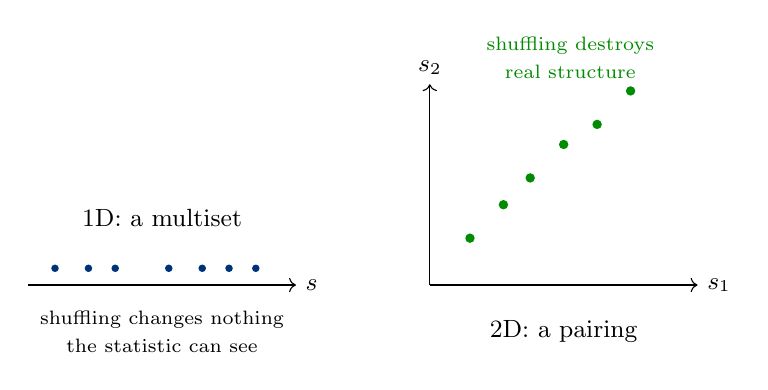
\begin{tikzpicture}[scale=0.85]
  \begin{scope}
    \draw[->] (0,0) -- (4,0) node[right] {\small $s$};
    \foreach \x in {0.4,0.9,1.3,2.1,2.6,3.0,3.4} \fill[kishblue] (\x,0.25) circle (1.6pt);
    \node at (2,1.0) {\small 1D: a multiset};
    \node[align=center] at (2,-0.7) {\scriptsize shuffling changes nothing\\[-2pt]\scriptsize the statistic can see};
  \end{scope}
  \begin{scope}[xshift=6cm]
    \draw[->] (0,0) -- (4,0) node[right] {\small $s_1$};
    \draw[->] (0,0) -- (0,3) node[above] {\small $s_2$};
    \foreach \p in {(0.6,0.7),(1.1,1.2),(1.5,1.6),(2.0,2.1),(2.5,2.4),(3.0,2.9)}
      \fill[signalgreen] \p circle (2pt);
    \node at (2,-0.7) {\small 2D: a pairing};
    \node[align=center, signalgreen] at (2.1,3.4) {\scriptsize shuffling destroys\\[-2pt]\scriptsize real structure};
  \end{scope}
\end{tikzpicture}
\caption{Why Erratum 1 is a finding the 2D design needs rather than only a defect. In one
dimension there is no pairing to destroy. In two there is, and the scramble becomes a genuine
null --- load-bearing from the first commit of the 2D engine.}
\end{figure}

\subsection{Standing Requirements for the 2D Engine}

\begin{enumerate}
    \item \textbf{Immutable from the 1D engine.} No shared code.
    \item \textbf{Form A re-derived in 2D} before any 2D lock is trusted. The theorem is a 1D
          result and does not automatically extend.
    \item \textbf{The scramble null wired in from the start.}
    \item \textbf{Synthetic calibration before real data.} Six lakes, expectations filed in
          advance, and the engine does not touch a real 2D lake until all six return their
          pre-registered result.
\end{enumerate}

\begin{predictionbox}
\textbf{The calibration set.}

\medskip
\begin{tabular}{@{}llp{0.42\textwidth}@{}}
\toprule
& \textbf{Construction} & \textbf{Pre-registered expectation} \\
\midrule
C1 & both coordinates uniform & null; $\lvert z\rvert < 3$ throughout \\
C2 & both log-normal, no harmonic relation & \textbf{null} --- the direct shape-artifact test \\
C3 & 30\% placed on a chosen register & strong lock at that register \emph{and nowhere else} \\
C4 & C3 with jitter at $1.5\times$ tolerance & degraded but detectable; calibrates sensitivity \\
C5 & C3 with one coordinate shuffled & \textbf{null} --- closes the loop Erratum 1 left open \\
C6 & C3 scaled below the lock floor & reports \textsc{out-of-range}, not null \\
\bottomrule
\end{tabular}

\medskip
\noindent The planted register is $19/\pi$, chosen deliberately away from $16/\pi$: planting at
the framework's own register and finding it would establish nothing we could trust about
ourselves. At least one lake carries a pre-registered \textbf{expected fail} --- a panel of six
passes proves the instrument agrees with itself, not that it can disagree.
\end{predictionbox}

\section{Closing}

The honest one-sentence summary of this volume is that we built an instrument, discovered it had
five ways of lying to us, fixed them, and nine domains were still standing.

That is a shorter ledger than Volume 11 carried and a better one. The reader who matters is the
one looking for the flaw, and this volume hands them the five we already found, with the
corrections, before they go looking.

The work ahead is a rebuild of the one-dimensional lakes under the boundaries of Chapter 5,
a permutation test aimed squarely at our own headline claim, and then two dimensions --- where
the null we have been carrying uselessly for eleven volumes finally does the job it was named
for.

% ==============================================================================
\chapter{The Reduction: What the Framework Actually Asks}
% ==============================================================================

\section{A Question Asked Sideways}

Chapters 3 through 8 repaired an instrument. This chapter asks what the instrument was
measuring, and the answer turns out to explain most of the repairs.

Strip the scalarization back to its arithmetic. With
\[
s = \frac{\ln\!\left(1 + x/x_0\right)}{\ln \kgeo}, \qquad r_p = \frac{24\pi s}{N},
\]
a record locks when $r_p$ falls within tolerance of an integer. Substitute and the condition
becomes

\begin{equation}
\ln\!\left(1 + \frac{x}{x_0}\right) \ \text{is a multiple of} \
\Delta_N \;=\; \frac{N \ln \kgeo}{24\pi} \;=\; N \times 0.0215902 .
\label{eq:deltaN}
\end{equation}

\begin{signalbox}
\textbf{The entire framework asks one question: is $\log x$ periodic with period $\Delta_N$?}

\medskip
\noindent The container of 24, the modulus, the offset $x_0$, the register index --- all of it
is machinery for asking that. Nothing else is being tested.
\end{signalbox}

Seeing it stated that plainly took eleven volumes, and it should have taken one. But the
statement is worth the delay, because once the question is written in that form the five
artifact forms of Chapter 4 stop looking like five separate accidents.

\section{Four of Five Reduce to One Root}

A periodic structure has two independent properties: a \emph{period}, which is how far apart
the repeats sit, and a \emph{phase}, which is where the repeats fall relative to some chosen
origin. They are different quantities and they carry very different amounts of physical
meaning.

\begin{table}[H]
\centering
\small
\begin{tabular}{@{}lp{0.42\textwidth}l@{}}
\toprule
\textbf{Artifact} & \textbf{Mechanism} & \textbf{Root} \\
\midrule
Unit dependence (Erratum 4f) & $\ln(cx) = \ln x + \ln c$ & additive \textbf{phase} shift \\
$x_0$ arbitrariness & the same additive shift & $x_0$ \emph{is} the phase origin \\
Form D, the lock floor & \texttt{nearest = max(1, round($r_p$))} & a hard, \textbf{phase-anchored} cut \\
The $\{4,8,16\}$ family & $24\pi \ln 2 / \ln \kgeo = 32.10 \approx 2^5$ & phase commensurability \\
Null-support mismatch & uniform null over the empirical range & the null must model support \\
\bottomrule
\end{tabular}
\caption{The artifact taxonomy, re-sorted by root cause rather than by symptom.}
\end{table}

\begin{warningbox}
\textbf{Four of the five reduce to the same thing: the statistic measures phase.}

\medskip
\noindent And phase is precisely the quantity that carries no physical content. It is fixed by
our choice of unit --- MeV or eV, hours or seconds --- and by our choice of $x_0$. Two decisions
that no physics constrains.

\medskip
\noindent \textbf{We built an instrument to measure the one property of the signal that we
ourselves supply.}
\end{warningbox}

\begin{figure}[H]
\centering
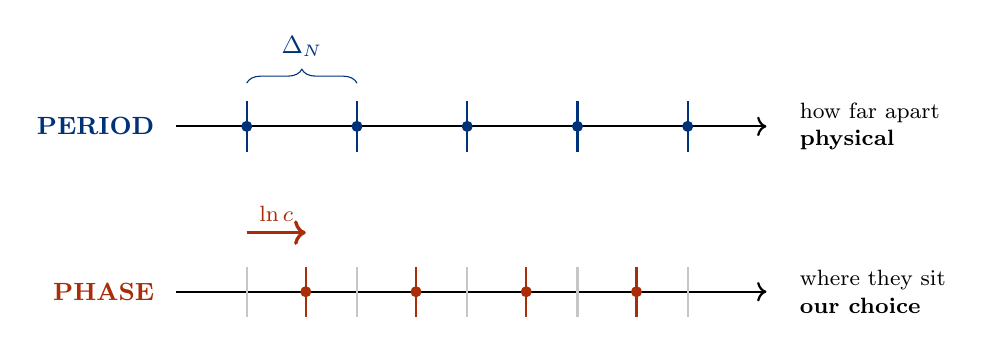
\begin{tikzpicture}[scale=1.0]
  % Period panel
  \begin{scope}
    \draw[->, thick] (-0.3,0) -- (7.2,0);
    \foreach \x in {0.6,2.0,3.4,4.8,6.2} {
      \draw[thick, kishblue] (\x,-0.32) -- (\x,0.32);
      \fill[kishblue] (\x,0) circle (2pt);
    }
    \draw[decorate, decoration={brace, amplitude=5pt}, kishblue]
         (0.6,0.55) -- (2.0,0.55) node[midway, above=6pt] {\small $\Delta_N$};
    \node[left, kishblue] at (-0.45,0) {\small\bfseries PERIOD};
    \node[align=left, anchor=west] at (7.5,0)
      {\footnotesize how far apart\\[-2pt]\footnotesize \textbf{physical}};
  \end{scope}
  % Phase panel
  \begin{scope}[yshift=-2.1cm]
    \draw[->, thick] (-0.3,0) -- (7.2,0);
    \foreach \x in {0.6,2.0,3.4,4.8,6.2} {
      \draw[thick, gray!45] (\x,-0.32) -- (\x,0.32);
    }
    \foreach \x in {1.35,2.75,4.15,5.55} {
      \draw[thick, cruciblered] (\x,-0.32) -- (\x,0.32);
      \fill[cruciblered] (\x,0) circle (2pt);
    }
    \draw[->, very thick, cruciblered] (0.6,0.75) -- (1.35,0.75)
          node[midway, above] {\footnotesize $\ln c$};
    \node[left, cruciblered] at (-0.45,0) {\small\bfseries PHASE};
    \node[align=left, anchor=west] at (7.5,0)
      {\footnotesize where they sit\\[-2pt]\footnotesize \textbf{our choice}};
  \end{scope}
\end{tikzpicture}
\caption{The same structure, two properties. The spacing between repeats is a property of the
data. Their absolute position is set by the unit in which the quantity happens to be recorded:
changing from MeV to eV slides every tick by $\ln c / \ln \kgeo$ and changes nothing physical.
Volumes 1 through 12 measured the lower panel.}
\label{fig:phaseperiod}
\end{figure}

\section{Old World, New World}

\oldworld{Spectroscopy names a line by where it falls. The sodium D doublet sits at 589.0 and
589.6 nanometres, and those numbers mean something because everyone agrees on the nanometre.
Position is the measurement.}

\newworld{A geometric harmonic register is not a position. It is a \emph{spacing} in
logarithmic coordinates. The quantity that carries the claim is how far apart the structure
repeats --- and that quantity survives a change of unit, while position does not.

\medskip
Volumes 1 through 11 tested the framework's claim using a statistic anchored to position. It
found real structure, repeatedly, in domains where structure exists. But it also inherited
every artifact that a position-anchored test can inherit, and Chapter 4 is the list.}

The remainder of this volume develops a second statistic that tests the upper panel of
Figure~\ref{fig:phaseperiod} and never touches the lower one. It is not a replacement. It is a second exposure of
the same hypothesis, with failure modes that are largely disjoint from the first --- and, as
Chapters 12 and 13 will show, with limits of its own that turn out to have applied to the
first statistic all along without anyone checking.

\section{A Note on How This Was Found}

The reduction in Equation~\ref{eq:deltaN} is three lines of substitution. It was available at
Volume 1. It was written down in Volume 12, in the fourth week of an audit that began because a
routine two-lake regression test produced a domain mean matching a constant stored inside the
lake.

We record that not as self-criticism but as a fact about how instruments are understood. The
question a measurement asks is often clearest after you have spent a month finding out what it
answers when nothing is there.

% ==============================================================================
\chapter{The Period Engine: What It Removes by Proof}
% ==============================================================================

\section{The Statistic}

If the question is whether $\log x$ repeats with period $\Delta_N$, the natural instrument is
the one periodicity detection has used for a century: map each record onto a circle whose
circumference is one period, and ask whether the resulting directions add up
\cite{rayleigh1880, mardia2000, fisher1993}.

\begin{equation}
\theta_j \;=\; \frac{2\pi \ln x_j}{\Delta_N}, \qquad
R \;=\; \left| \frac{1}{n}\sum_{j=1}^{n} e^{i\theta_j} \right|, \qquad
P \;=\; nR^2 .
\label{eq:rayleigh}
\end{equation}

$R$ is the length of the mean unit vector --- the \emph{circular resultant}. If the phases are
scattered, the vectors cancel and $R \to 0$. If they cluster, the vectors reinforce and
$R \to 1$. The record's position on the circle is used; its position on the line is not.

\begin{figure}[H]
\centering
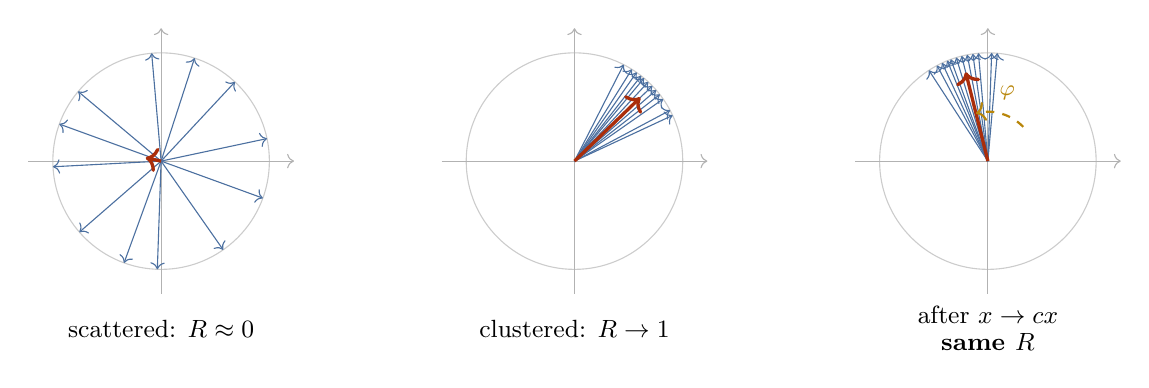
\begin{tikzpicture}[scale=1.25]
  \begin{scope}
    \draw[gray!40] (0,0) circle (1.1);
    \draw[->, gray!60] (-1.35,0) -- (1.35,0);
    \draw[->, gray!60] (0,-1.35) -- (0,1.35);
    \foreach \a in {12,47,95,140,183,221,268,305,340,72,160,250} {
      \draw[kishblue!70, ->, thin] (0,0) -- (\a:1.1);
    }
    \draw[->, very thick, cruciblered] (0,0) -- (168:0.16);
    \node at (0,-1.7) {\small scattered: $R \approx 0$};
  \end{scope}
  \begin{scope}[xshift=4.2cm]
    \draw[gray!40] (0,0) circle (1.1);
    \draw[->, gray!60] (-1.35,0) -- (1.35,0);
    \draw[->, gray!60] (0,-1.35) -- (0,1.35);
    \foreach \a in {28,35,41,47,52,58,63,25,44,55,38,50} {
      \draw[kishblue!70, ->, thin] (0,0) -- (\a:1.1);
    }
    \draw[->, very thick, cruciblered] (0,0) -- (44:0.93);
    \node at (0,-1.7) {\small clustered: $R \to 1$};
  \end{scope}
  \begin{scope}[xshift=8.4cm]
    \draw[gray!40] (0,0) circle (1.1);
    \draw[->, gray!60] (-1.35,0) -- (1.35,0);
    \draw[->, gray!60] (0,-1.35) -- (0,1.35);
    \foreach \a in {88,95,101,107,112,118,123,85,104,115,98,110} {
      \draw[kishblue!70, ->, thin] (0,0) -- (\a:1.1);
    }
    \draw[->, very thick, cruciblered] (0,0) -- (104:0.93);
    \draw[->, thick, goldseal, dashed] (44:0.5) arc (44:104:0.5);
    \node[goldseal] at (74:0.72) {\footnotesize $\varphi$};
    \node[align=center] at (0,-1.7) {\small after $x \to cx$\\[-2pt]\small \textbf{same $R$}};
  \end{scope}
\end{tikzpicture}
\caption{The circular resultant, and why a change of unit cannot touch it. Multiplying every
value by $c$ adds the same constant $\varphi = 2\pi\ln c/\Delta_N$ to every phase. The whole
diagram rotates. The red resultant swings to a new direction and \textbf{keeps its length
exactly}.}
\end{figure}

\section{Unit Invariance, Proved}

This is the first claim in the programme closed by algebra rather than by measurement, and it
is worth writing out.

\begin{signalbox}
\textbf{Theorem (unit invariance).} Let $x \to cx$ for any $c > 0$. Then $P$ is unchanged.

\medskip
\textbf{Proof.} $\theta_j \to \dfrac{2\pi \ln(c x_j)}{\Delta_N} = \theta_j + \varphi$ with
$\varphi = \dfrac{2\pi \ln c}{\Delta_N}$, the same for every $j$. Hence
\[
\sum_j e^{i(\theta_j + \varphi)} \;=\; e^{i\varphi} \sum_j e^{i\theta_j},
\qquad
\left| e^{i\varphi} \right| = 1 ,
\]
so $R$, and therefore $P = nR^2$, is unchanged. $\square$
\end{signalbox}

Measured against the phase statistic on the same data:

\begin{table}[H]
\centering
\small
\begin{tabular}{@{}lrr@{}}
\toprule
\textbf{Unit factor} & \textbf{phase engine lock rate} & \textbf{period engine $P$} \\
\midrule
$\times 1$ (as promoted) & 0.18860 & 4950.5 \\
$\times 3$ & 0.08765 & 4950.5 \\
$\times 7$ & 0.08945 & 4950.5 \\
$\times 10$ & 0.08533 & 4950.5 \\
$\times e$ & 0.08840 & 4950.5 \\
$/60$ & 0.11135 & 4950.5 \\
\bottomrule
\end{tabular}
\caption{The same 200{,}000-record synthetic lake with a lock planted at $19/\pi$, expressed in
six different units. The phase statistic swings by more than a factor of two. The period
statistic is identical to one decimal place --- as the theorem requires.}
\end{table}

\begin{warningbox}
Erratum 4f established that every cross-domain register agreement in the Rosetta Atlas rested on
unit choices that were never pre-registered --- and that expressing nuclear binding energy in eV
rather than MeV displaces its phase by 0.47 of a period, the maximum possible.

\medskip
\noindent \textbf{Under the period statistic that objection does not arise.} A bridge that holds
holds in every unit system simultaneously. Erratum 4f acquires a remedy rather than only a
diagnosis.
\end{warningbox}

\section{What Disappears}

\begin{table}[H]
\centering
\small
\begin{tabular}{@{}lll@{}}
\toprule
\textbf{Stage} & \textbf{Phase engine} & \textbf{Period engine} \\
\midrule
scalarize & $\ln(1+x/x_0)/\ln \kgeo$; modulus baked in & none; raw $x$ stored \\
$x_0$ & required, per-domain, pre-registered & \textbf{none} \\
chaos null & 100 MC trials per domain per register & none \\
synthetic null & Gaussian matched and clipped & none \\
scramble null & written, never read; inert in 1D & none \\
common support & drop $r_p < 0.5$ from both arms & \textbf{none --- no clamp exists} \\
offset-sweep baseline & 24 phases per register & none --- phase is not measured \\
null estimation & separate Monte Carlo stage & empirical background, inside the statistic \\
\bottomrule
\end{tabular}
\caption{What the period engine does not carry. Three of these were the mechanisms of Forms C
and D.}
\end{table}

\begin{itemize}
    \item \textbf{$x_0$ disappears.} There is no offset to choose, pre-register, or defend.
          The parameter that Chapter 5 showed had never been used --- $x_0 = 1.0$ across all 74
          domains regardless of the natural scale of the quantity --- has no analogue here.
    \item \textbf{The lock floor disappears.} There is no
          \texttt{nearest = max(1, round($r_p$))} and therefore no mechanically non-lockable
          region. Every positive record contributes a unit vector at its own phase.
          \textbf{Form D has no mechanism to act through.}
    \item \textbf{The $\{4,8,16\}$ commensurability disappears} as a phase effect, though
          Chapter 13 shows it returns in a different guise through range edges.
\end{itemize}

\section{Zeros, and Why Their Handling Is Forced}

$\log x$ requires $x > 0$. Records at exactly zero are excluded and the count published.

This is not a choice dressed as a principle. Any additive offset $x \to x + \epsilon$ would
destroy the very invariance that justifies the statistic, since $\ln(cx + \epsilon)$ is not
$\ln(cx) + \text{const}$. \textbf{There is no admissible offset.} A zero has no logarithm, and a
domain must state how many it discarded.

Two of the five domains recovered in Chapter 14 --- \texttt{orbital\_eccentricity} and
\texttt{galactic\_sersic} --- have ranges beginning at zero. Their post-exclusion span, and
therefore their resolution ceiling, is published before they are scored.

\section{The Data Product Stops Carrying the Hypothesis}

This consequence has nothing to do with artifacts and may outlast them.

Under the phase formulation, $\kgeo$ is applied at promotion. Every record in every scalarized
lake carries the modulus baked into it. The data product and the hypothesis are entangled: a
reader who doubts the hypothesis cannot use the data.

Under the period formulation, the promoted lake stores \textbf{raw $x$ with documented units}.
The logarithm and the modulus are both applied at test time.

\begin{signalbox}
\textbf{The lake becomes framework-agnostic.} A sceptic may take our published lakes and test
any modulus they like, or none at all --- Benford structure \cite{benford1938, hill1995},
log-periodic corrections from discrete scale invariance \cite{sornette1998}, or a hypothesis we
have not thought of.

\medskip
\noindent That is a credibility asset the previous architecture could not offer at any price.
\end{signalbox}

% ==============================================================================
\chapter{What the Period Engine Cannot Do}
% ==============================================================================

\section{A Chapter Written Against Ourselves}

The previous chapter is the case for the period engine. This one is the case against it, and it
is longer.

It contains three results. The first is that a claim made in the first draft of the design ---
that the engine needs no null --- was wrong. The second is that the correction for the first
introduces a background estimate with very few independent samples. The third is the most
important finding in this volume, and it is not about the period engine at all.

\section{The Null Was Not Removed. It Was Replaced.}

The first specification claimed that under uniform phase $2nR^2 \sim \chi^2_2$ exactly, so the
null is closed-form and no Monte Carlo stage is required.

That claim does not survive contact with a finite dataset.

Consider a perfectly structureless domain: $\ln x$ uniform over a span $L$. Write $M = L/\Delta_N$
for the number of periods spanned. The resultant is not zero, because a uniform density over a
non-integer number of periods does not close on itself:

\begin{equation}
R \;=\; \left| \frac{\sin(\pi M)}{\pi M} \right|, \qquad
P_{\text{leak}} \;=\; n\,\frac{\sin^2(\pi M)}{(\pi M)^2} .
\label{eq:leak}
\end{equation}

This is not an approximation fitted to a fixture. It is the closed form of the continuous
integral, and it was verified against simulation across four combinations of $n$ and span.

\begin{table}[H]
\centering
\small
\begin{tabular}{@{}rrrrr@{}}
\toprule
$n$ & span & $M$ & \textbf{predicted $P$} & \textbf{measured $P$} \\
\midrule
50{,}000 & 12 & 34.7 & 8.5 & 8.5 \\
200{,}000 & 12 & 34.7 & 34.1 & 34.1 \\
500{,}000 & 12 & 34.7 & 85.2 & 85.4 \\
200{,}000 & 26 & 75.3 & 3.6 & 3.6 \\
\bottomrule
\end{tabular}
\caption{Edge leakage is deterministic and scales with $n$.}
\end{table}

\begin{warningbox}
The analytic $\chi^2_2$ null has expectation $\mathbb{E}[P] = 1$. Structureless data at
$n = 2\times10^5$ returns $P \approx 34$. \textbf{The analytic null is unusable at survey
scale.}

\medskip
\noindent It is valid only when $n/(\pi M)^2 \ll 1$, i.e. $M \gg \sqrt{n}/\pi$: about
\textbf{142 periods} at $n = 2\times10^5$ and \textbf{427} at $n = 1.8\times10^6$. No domain in
the survey spans a tenth of that.

\medskip
\noindent The null generation moved from a separate stage into the statistic. \textbf{It did not
disappear}, and the first draft of this design said it had.
\end{warningbox}

We record this in the same register as the scramble tier of Erratum 1 --- a null described as
doing work it was not doing. The difference is that this one was caught before it was filed,
by the referee, from an internal inconsistency between two numbers in the same document.

\section{The Annular Background}

The leakage must therefore be estimated from the data. The estimate is the power at
\emph{neighbouring} periods: leakage varies smoothly with period, structure at $\Delta_N$ does
not, so the difference isolates the signal.

The first attempt used a window of $\pm 35\%$ in period. That window, at $19/\pi$, spans
registers 12.4 to 25.7 --- most of the family. The background was contaminated by other
registers, and any domain locking across a band would have had its own signal subtracted.

Narrowing the window to clear the adjacent register then failed in the opposite direction: the
window fell inside the peak's own width, the background rose to the peak level, and a planted
lock collapsed from an excess of $+482$ to $+1.5$.

The background must therefore be an \textbf{annulus}, bounded on both sides.

\begin{figure}[H]
\centering
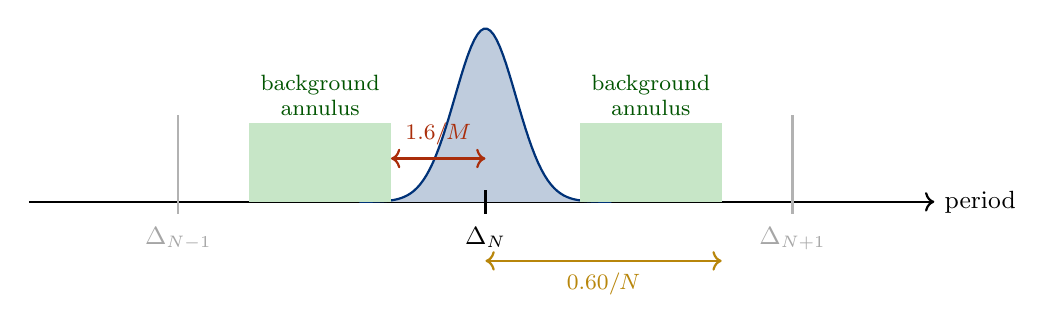
\begin{tikzpicture}[scale=1.0]
  \draw[->, thick] (-0.3,0) -- (11.2,0) node[right] {\small period};
  % peak
  \fill[kishblue!25] plot[domain=4.1:6.9, samples=60]
      ({\x}, {2.2*exp(-((\x-5.5)^2)/0.30)}) -- (6.9,0) -- (4.1,0) -- cycle;
  \draw[thick, kishblue] plot[domain=3.9:7.1, samples=80]
      ({\x}, {2.2*exp(-((\x-5.5)^2)/0.30)});
  \draw[thick] (5.5,-0.15) -- (5.5,0.15);
  \node[below] at (5.5,-0.2) {\small $\Delta_N$};
  % adjacent registers
  \foreach \x/\l in {1.6/{$\Delta_{N-1}$}, 9.4/{$\Delta_{N+1}$}} {
    \draw[thick, gray!60] (\x,-0.15) -- (\x,1.1);
    \node[below, gray!70] at (\x,-0.2) {\small \l};
  }
  % annulus bands
  \fill[signalgreen!22] (2.5,0) rectangle (4.3,1.0);
  \fill[signalgreen!22] (6.7,0) rectangle (8.5,1.0);
  \node[signalgreen!60!black, align=center] at (3.4,1.35) {\footnotesize background\\[-3pt]\footnotesize annulus};
  \node[signalgreen!60!black, align=center] at (7.6,1.35) {\footnotesize background\\[-3pt]\footnotesize annulus};
  \draw[<->, cruciblered, thick] (4.3,0.55) -- (5.5,0.55);
  \node[cruciblered, above] at (4.9,0.6) {\footnotesize $1.6/M$};
  \draw[<->, goldseal, thick] (5.5,-0.75) -- (8.5,-0.75);
  \node[goldseal, below] at (7.0,-0.78) {\footnotesize $0.60/N$};
\end{tikzpicture}
\caption{The background annulus. Its inner radius must clear the peak's own fractional width
$1/M$; its outer radius must stop short of the adjacent register at $1/N$. Both constraints are
hard, and \textbf{the annulus exists only if the peak is narrower than the register spacing}.}
\end{figure}

\begin{table}[H]
\centering
\small
\begin{tabular}{@{}llp{0.40\textwidth}@{}}
\toprule
\textbf{Bound} & \textbf{Value} & \textbf{Purpose} \\
\midrule
inner radius & $1.6/M$ & clears the peak's own width \\
outer radius & $0.60/N$ & never reaches register $N \pm 1$ \\
samples & 121, split either side & \\
\midrule
\textbf{non-empty when} & $M/N > 1.6/0.60 = \mathbf{2.67}$ & \\
\bottomrule
\end{tabular}
\end{table}

\subsection{Provenance and sensitivity of the two constants}

The values 1.6 and 0.60 were calibrated on a synthetic fixture, after the $\pm 35\%$ window
failed, and before any real-data result was seen. That provenance belongs in the record, not in
a lab note. And because two fixture-calibrated numbers now decide which domains produce results
at all, the sensitivity is published:

\begin{table}[H]
\centering
\small
\begin{tabular}{@{}lrr@{}}
\toprule
\textbf{inner / outer} & \textbf{threshold} & \textbf{domains scoreable of 9} \\
\midrule
1.4 / 0.70 & 2.00 & 1 \\
1.8 / 0.70 & 2.57 & 1 \\
\textbf{1.6 / 0.60} & \textbf{2.67} & \textbf{1} \\
1.4 / 0.50 & 2.80 & 1 \\
1.8 / 0.50 & 3.60 & 1 \\
\bottomrule
\end{tabular}
\caption{The partition is invariant across the whole plausible parameter range. The gap between
the best domain (4.17) and the next (1.89) is structural, not a threshold artifact.}
\end{table}

\subsection{How many independent samples the annulus really has}

Periodogram ordinates are correlated over the peak's own width. Sampling 121 points inside one
correlation length does not give 121 independent estimates. The effective count per side is the
annulus width divided by the correlation width:

\begin{equation}
n_{\text{indep}} \;=\; 2\left( 0.60\,\frac{M}{N} - 1.6 \right).
\label{eq:nindep}
\end{equation}

For the best domain in the survey, at $M/N = 4.17$, this is \textbf{1.8 in total}. An earlier
draft quoted a 6.4\% uncertainty on the background estimate, computed as though there were 121
independent draws. That figure is \textbf{withdrawn}; the uncertainty is propagated from
Equation~\ref{eq:nindep} and published per domain per register.

\subsection{An open problem, recorded unsolved}

A log-phase surrogate null was proposed by the referee and tested by the architect. It
recovers planted locks at every register --- including those where the annulus is empty --- but
it returns \textbf{false positives up to $z = +55$ on structureless data}.

The reason is algebraic. $P$ depends only on the fractional parts:
\[
P = \left| \sum_j e^{2\pi i (k_j + f_j)} \right|^2 = \left| \sum_j e^{2\pi i f_j} \right|^2 ,
\]
and randomising $f$ uniformly within each period-bin gives $\int_0^1 e^{2\pi i f}\,df = 0$
exactly. The coherent term is annihilated by construction, so the surrogate reports the
$\chi^2_2$ mean of 1.0 while the real structureless power sits at 10 to 55.

\begin{warningbox}
The obstruction generalises past that implementation. \textbf{Leakage and signal are the same
Fourier component} --- the amplitude of the density at frequency $1/\Delta_N$. Any resampling
that removes power there removes both. \emph{There is no surrogate that separates them.}

\medskip
\noindent What does separate them is that leakage is predictable from the coarse density and
signal is not. A candidate analytic edge correction therefore exists in principle. It has not
been derived or validated, and it is recorded here as an open problem rather than proposed as a
solution.
\end{warningbox}

\section{The Resolution Criterion}

Everything above is about the period engine. This section is not.

The annulus requires the peak to be narrower than the register spacing. A coherent peak has
fractional width $\sim 1/M$; adjacent registers are separated by $1/N$, since
$\Delta_N \propto N$. The annulus therefore exists only when $1/M < 1/N$, which rearranges to

\begin{equation}
\boxed{\ \ \text{log-span} \;>\; N^{2}\,\frac{\ln \kgeo}{24\pi} \;=\; N^{2} \times 0.021590 \ \ }
\label{eq:resolution}
\end{equation}

\begin{signalbox}
\textbf{This is the standard Rayleigh resolution criterion} \cite{rayleigh1879, bracewell2000},
and it is \textbf{a property of the data, not of the statistic}.

\medskip
\noindent To distinguish register $N$ from register $N+1$, a domain must span enough orders of
magnitude. Not enough \emph{records} --- enough \emph{range}. \textbf{The phase engine is
subject to it identically and has never checked.}
\end{signalbox}

\begin{figure}[H]
\centering
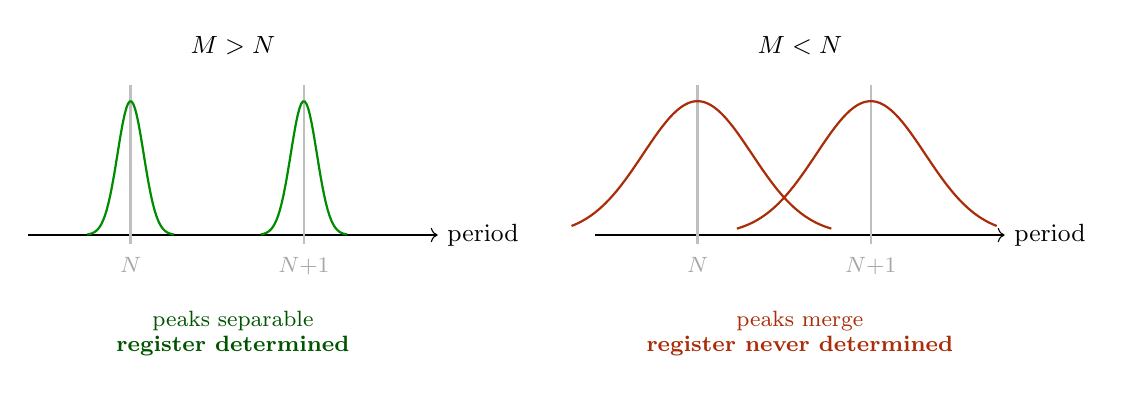
\begin{tikzpicture}[scale=1.0]
  \begin{scope}
    \draw[->] (0,0) -- (5.2,0) node[right] {\small period};
    \draw[thick, gray!50] (1.3,-0.12) -- (1.3,1.9);
    \draw[thick, gray!50] (3.5,-0.12) -- (3.5,1.9);
    \node[below, gray!70] at (1.3,-0.16) {\footnotesize $N$};
    \node[below, gray!70] at (3.5,-0.16) {\footnotesize $N{+}1$};
    \draw[thick, signalgreen] plot[domain=0.75:1.85, samples=50]
        ({\x}, {1.7*exp(-((\x-1.3)^2)/0.055)});
    \draw[thick, signalgreen] plot[domain=2.95:4.05, samples=50]
        ({\x}, {1.7*exp(-((\x-3.5)^2)/0.055)});
    \node[align=center] at (2.6,2.4) {\small $M > N$};
    \node[align=center, signalgreen!60!black] at (2.6,-1.25) {\footnotesize peaks separable\\[-3pt]\footnotesize \textbf{register determined}};
  \end{scope}
  \begin{scope}[xshift=7.2cm]
    \draw[->] (0,0) -- (5.2,0) node[right] {\small period};
    \draw[thick, gray!50] (1.3,-0.12) -- (1.3,1.9);
    \draw[thick, gray!50] (3.5,-0.12) -- (3.5,1.9);
    \node[below, gray!70] at (1.3,-0.16) {\footnotesize $N$};
    \node[below, gray!70] at (3.5,-0.16) {\footnotesize $N{+}1$};
    \draw[thick, cruciblered] plot[domain=-0.3:3.0, samples=70]
        ({\x}, {1.7*exp(-((\x-1.3)^2)/0.95)});
    \draw[thick, cruciblered] plot[domain=1.8:5.1, samples=70]
        ({\x}, {1.7*exp(-((\x-3.5)^2)/0.95)});
    \node[align=center] at (2.6,2.4) {\small $M < N$};
    \node[align=center, cruciblered] at (2.6,-1.25) {\footnotesize peaks merge\\[-3pt]\footnotesize \textbf{register never determined}};
  \end{scope}
\end{tikzpicture}
\caption{The diffraction limit of a harmonic survey. When the data spans too few periods the
peak is wider than the register spacing, and no statistic, no null and no number of records can
say which register the structure occupies.}
\end{figure}

\subsection{Applied to the nine surviving domains}

\begin{table}[H]
\centering
\small
\begin{tabular}{@{}lrrrrl@{}}
\toprule
\textbf{Domain} & \textbf{Reg.} & \textbf{log-span} & $M$ & $M/N$ & \textbf{Status} \\
\midrule
\texttt{quantum\_transitional} & $16/\pi$ & 23.04 & 66.7 & \textbf{4.17} & \textbf{scoreable} \\
\texttt{subnuclear\_mass} & $13/\pi$ & 6.90 & 24.6 & 1.89 & background-limited \\
\texttt{orbital} & $22/\pi$ & 15.16 & 31.9 & 1.45 & background-limited \\
\texttt{stellar\_colour} & $15/\pi$ & 6.21 & 19.2 & 1.28 & background-limited \\
\texttt{galactic\_mass} & $19/\pi$ & 9.93 & 24.2 & 1.27 & background-limited \\
\texttt{galactic} & $18/\pi$ & 6.40 & 16.5 & 0.91 & \textbf{resolution-limited} \\
\texttt{subnuclear\_pt\_lead} & $26/\pi$ & 7.23 & 12.9 & 0.50 & \textbf{resolution-limited} \\
\texttt{subnuclear\_pt\_sublead} & $26/\pi$ & 6.65 & 11.8 & 0.46 & \textbf{resolution-limited} \\
\texttt{cosmology} & $15/\pi$ & 0.47 & 1.4 & 0.10 & \textbf{resolution-limited} \\
\bottomrule
\end{tabular}
\caption{Two distinct failures. \textsc{resolution-limited} ($M/N < 1$) is permanent: the data
cannot distinguish the claimed register from its neighbour. \textsc{background-limited}
($1 < M/N < 2.67$) is a to-do: the register is resolvable but the annulus is too thin to sample.}
\end{table}

\begin{warningbox}
\textbf{Four of the nine surviving domains cannot distinguish their reported register from its
neighbour using their own dynamic range.} That is a statement about Volumes 5 through 12, not
about the period engine.

\medskip
\noindent \textbf{The period engine, as specified, can score exactly one domain of nine.}
\end{warningbox}

\subsection{It converges with an earlier verdict from an unrelated direction}

Chapter 3 established that at $T = 100$ chaos trials the run-to-run uncertainty on a $z$ of
magnitude 90 is $\pm 6.8$, so the Volume 11 separation of $15/\pi$ ($+98.3$) from $16/\pi$
($+94.0$) --- a gap of 4.3 --- was never measurable. Equation~\ref{eq:resolution} says the same
domain, at $M/N = 1.15$, could never have distinguished those registers regardless of trial
count.

\begin{signalbox}
Two independent routes --- finite trial count and finite dynamic range --- reach the same
verdict on the same claim. That is the strongest form such a verdict can take.
\end{signalbox}

\subsection{Consequences adopted}

\begin{enumerate}
    \item \textbf{Published per domain, per register, for both engines.} No register claim is
          admissible without its $M/N$ printed beside it.
    \item \textbf{A promotion criterion.} Every future lake states its log-span and its $M/N$ at
          the registers it will be tested at, \emph{before} promotion. A lake that cannot resolve
          the register it is being promoted to test is not promoted.
    \item \textbf{Inherited by the 2D engine.} Both coordinates carry their own requirement and
          the joint requirement is at least as strict as the stricter of the two. This is built
          into the 2D design from the start rather than discovered inside it --- which is, in the
          end, the most valuable thing this chapter produces.
\end{enumerate}

\subsection{And it reaches the bridges}

Most physical quantities span two to four orders of magnitude, giving log-spans of 4.6 to 9.2.
At $N = 20$, Equation~\ref{eq:resolution} demands a log-span above 8.6.

Rosetta Bridge~1 asserts that nuclear binding energy and galactic velocity dispersion share
$21/\pi$. Binding energy per nucleon runs from roughly 1 to 9~MeV, a log-span of 2.20, giving
$M/N = 0.23$. SDSS velocity dispersions run from roughly 50 to 400~km/s, a log-span of 2.08,
giving $M/N = 0.22$.

\begin{erratumbox}
\textbf{Bridge 1 is register-unresolved from both ends.} Neither domain has the dynamic range to
distinguish $21/\pi$ from $20/\pi$ or $22/\pi$.

\medskip
\noindent An unresolved register is not a \emph{wrong} register. It is a claim the data was
never able to make. Some bridges may hold at native resolution once their domains are rebuilt
from source with fuller range. That is a rebuild, not a retraction --- but it is not a claim
until the rebuild is done.
\end{erratumbox}

$M/N$ is computed for every domain in every bridge of the Rosetta Atlas as a condition of
Erratum 4. It is arithmetic on quantities already in hand and requires no run.

% ==============================================================================
\chapter{The Degeneracy, and What the Data Can Determine}
% ==============================================================================

\section{A Question That Answered Itself}

While testing whether atomic structure could account for the surviving anchor, the architect
raised what he believed was an untested question: has the scalarization modulus $\kgeo$ itself
ever been varied, as opposed to the register index $N$?

The founder's recollection was that sweeps at $15/\pi$, $16/\pi$ and $17/\pi$ had been run. The
referee confirmed it from the record: Volume 5 tested exactly those three candidates, Volume 6
expanded to eleven, Volume 7 to twenty-two, and the numbers survive --- the quantum domain
returned $z = -10.57$, $-16.93$ and $-16.04$ at $15/\pi$, $16/\pi$ and $17/\pi$ respectively.

The referee also established what was varied. Volume 6, describing the expansion: \emph{``Only
the moduli under test changed. Two lines of code.''} Two lines is the target list in the pinch
stage. Changing $\kgeo$ would re-scalarize every record in every lake --- a full pipeline
rebuild, not two lines.

\begin{correctionbox}
Both recollections were correct and they were not in conflict. A three-modulus sweep was run at
Volume 5; it varied the \emph{target register} $N/\pi$. The architect's claim that the
\emph{coordinate} $\kgeo$ has never been scanned as a separate experiment stands on the record.

\medskip
\noindent What neither party anticipated is that it never can be.
\end{correctionbox}

\section{The Degeneracy}

Write out both statistics and look at where the two constants appear.

\begin{align}
\text{Phase engine:} \quad & r_p = \frac{24\,s}{N/\pi} = \frac{24\pi \ln(1+x)}{N \ln \kgeo} \\[4pt]
\text{Period engine:} \quad & \theta = \frac{2\pi \ln x}{\Delta_N}, \qquad
\Delta_N = \frac{N \ln \kgeo}{24\pi}
\end{align}

\begin{signalbox}
\textbf{In both statistics, $N$ and $\ln \kgeo$ enter only through the product
$N \ln \kgeo$. Nowhere else.}

\medskip
\noindent Therefore a scan over $\kgeo$ at fixed $N$ and a scan over $N$ at fixed $\kgeo$ trace
the same one-parameter family. \textbf{They are the same experiment at different sample points.}
\end{signalbox}

\begin{figure}[H]
\centering
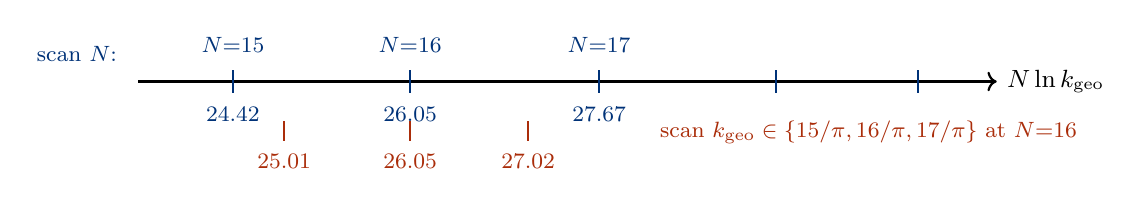
\begin{tikzpicture}[scale=1.0]
  \draw[->, thick] (-0.3,0) -- (10.6,0) node[right] {\small $N \ln \kgeo$};
  \foreach \v/\l in {0.9/24.42, 3.15/26.05, 5.55/27.67, 7.8/29.29, 9.6/30.91} {
    \draw[thick, kishblue] (\v,-0.14) -- (\v,0.14);
  }
  \node[below, kishblue] at (0.9,-0.2) {\footnotesize 24.42};
  \node[below, kishblue] at (3.15,-0.2) {\footnotesize 26.05};
  \node[below, kishblue] at (5.55,-0.2) {\footnotesize 27.67};
  \node[kishblue, above] at (0.9,0.25) {\footnotesize $N{=}15$};
  \node[kishblue, above] at (3.15,0.25) {\footnotesize $N{=}16$};
  \node[kishblue, above] at (5.55,0.25) {\footnotesize $N{=}17$};
  \node[left, kishblue] at (-0.45,0.35) {\footnotesize scan $N$:};

  \foreach \v in {1.55,3.15,4.65} {
    \draw[thick, cruciblered] (\v,-0.75) -- (\v,-0.5);
  }
  \node[below, cruciblered] at (1.55,-0.8) {\footnotesize 25.01};
  \node[below, cruciblered] at (3.15,-0.8) {\footnotesize 26.05};
  \node[below, cruciblered] at (4.65,-0.8) {\footnotesize 27.02};
  \node[cruciblered, align=left, anchor=west] at (6.2,-0.65)
       {\footnotesize scan $\kgeo \in \{15/\pi, 16/\pi, 17/\pi\}$ at $N{=}16$};
\end{tikzpicture}
\caption{One line, two samplings. Scanning the register index and scanning the coordinate move
along the identical axis. The data can identify a preferred \emph{product}; splitting that
product into ``register 16'' and ``coordinate $16/\pi$'' is a convention, not a measurement.}
\end{figure}

Three consequences, and they cut in different directions.

\begin{enumerate}
    \item \textbf{The coordinate has in fact been scanned densely, every run, since Volume 7.}
          The 23-register scan is not merely 23 candidate alternatives; it is a dense scan of the
          modulus axis itself. The framework has been tested against alternatives far more
          thoroughly than the architect's question implied.
    \item \textbf{A separate $\kgeo$ scan is therefore vacuous as a design.} It returns the
          register scan re-parameterised. It cannot be an independent test, and the proposal to
          run one is withdrawn.
    \item \textbf{And the framework cannot claim $\kgeo = 16/\pi$ from data.} Its specific value
          rests on the theoretical derivation --- sixteen internal tension modes, heterotic
          symmetry rank, closure constraints --- and on the convention that the kinematic
          primary is numbered 16. \emph{No sweep can supply it, and none ever could have.}
\end{enumerate}

\section{The Well-Posed Version: the Comb Test}

The degeneracy is not total. A \emph{single} peak cannot determine its own fundamental, but a
\emph{comb} of peaks determines its own spacing.

\begin{predictionbox}
\textbf{The comb test.} Scan the period continuously over a range spanning several registers ---
not at 23 discrete points, but densely. Ask:

\begin{itemize}
    \item Do the excess peaks fall on a comb of \emph{uniform} spacing $\Delta_0$?
    \item Is $\Delta_0$ consistent with $\ln \kgeo / 24\pi = 0.0215902$?
\end{itemize}

\textbf{Residual ambiguity, stated before running.} A comb determines its fundamental only up to
integer subdivision: a comb at spacing $\Delta_0$ is also a comb at $\Delta_0/2$ with alternate
teeth empty. Even the comb test fixes $\ln \kgeo$ only up to a rational factor.
\end{predictionbox}

This is the one construction that can see a comb rather than sampling 23 points on it, and it is
the natural task for a continuous period scan. It runs on \texttt{quantum\_transitional}, the one
scoreable domain.

\section{Two Bullets That Cannot Have Come From Any Run}

The Rosetta Atlas states, of the three-modulus sweep, that only $16/\pi$ produces \emph{maximal
lock rates, minimal residuals, stable harmonic clustering, correct Kolmogorov scaling, and
universal slipstream behavior}, concluding that \emph{no nearby modulus reproduces the observed
structure of the universe}.

\begin{erratumbox}
\textbf{Erratum 6.} No pipeline stage computes Kolmogorov scaling. No pipeline stage computes
slipstream behaviour. Those are Rosetta theory constructs, not outputs of
\texttt{build\_pinch\_table.py}. Whatever run produced the first three bullets did not produce
the last two.

\medskip
\noindent And the first bullet is contradicted by our own published tables. ``Only $16/\pi$
produces maximal lock rates'' fails against Volume 7's family table --- chemistry peaks at
$11/\pi$ with $z = 70$, galactic at $21/\pi$ with $z = 59$ --- and against Volume 11, where
\texttt{stellar\_colour} peaks at $20/\pi$ ($+124.5$) and protein backbone at $25/\pi$
($+157.2$). \textbf{Sixteen is not the maximal register.} It is one register among 23, and
several domains peak higher elsewhere.

\medskip
\noindent The passage is replaced by the Volume 5 three-target table with its actual $z$-values
shown, including the negative ones, and the two non-pipeline bullets are struck.
\end{erratumbox}

\section{A Pre-Registered Falsification Condition Appears to Be Met}

\emph{Noise Does Not Lock} files this as falsification condition~\#1:

\begin{quote}
\itshape The framework will be considered substantially undermined if the multi-modulus sweep
shows comparable peaks at multiple candidate moduli. If $15/\pi$, $16/\pi$, and $17/\pi$ all
produce maximum $z$-scores above 50, the modulus is not specific and the arbitrary constant
objection stands.
\end{quote}

Against Volume 11's published pinch table:

\begin{table}[H]
\centering
\small
\begin{tabular}{@{}lll@{}}
\toprule
\textbf{Register} & \textbf{Best published domain} & \textbf{$z$} \\
\midrule
$15/\pi$ & \texttt{stellar\_kinematic} & $\mathbf{+98.3}$ \\
$16/\pi$ & \texttt{galactic\_sersic} & $\mathbf{+343.4}$ \\
$17/\pi$ & \texttt{planetary\_atlantic} & $\mathbf{+121.6}$ \\
\bottomrule
\end{tabular}
\end{table}

\begin{erratumbox}
\textbf{All three exceed 50, two by more than a factor of two. On the published record,
falsification condition \#1 is met.}

\medskip
\noindent The caveat is substantial and must be stated with it: \emph{every domain in that
table is now compromised}. \texttt{stellar\_kinematic} is withdrawn under Erratum 4a.
\texttt{planetary\_atlantic} is suspended under Form E. \texttt{galactic\_sersic} is suspended
by the section below. The condition may therefore be met only by results this audit has already
set aside.

\medskip
\noindent That does not dissolve the problem. It relocates it. \textbf{Either the condition is
met and must be reported as met, or the domains meeting it are artifacts and it must be
re-evaluated on the surviving portrait after regeneration.} Both paths require the check to be
run and its status stated. What is not available is leaving a pre-registered falsification
condition unevaluated when its trigger is visible in our own published table.
\end{erratumbox}

Condition \#1 is formally re-evaluated as part of the Volume 11 regeneration, and its status is
recorded in Erratum 4 whichever way it lands.

\section{\texttt{galactic\_sersic}: the Same Arithmetic by a Second Route}

Checking the falsification condition turned up a new Form E case, and it is the cleanest
published example of the $\{4,8,16\}$ mechanism in the survey.

Volume 11 row 36, \texttt{galactic\_sersic}, $n = 59{,}563$, chaos $z$ across all 23 registers:

\begin{center}
\small
$4/\pi$: $\mathbf{+321.3}$ \quad $8/\pi$: $\mathbf{+298.6}$ \quad $16/\pi$: $\mathbf{+343.4}$
\quad \emph{every other register between $-8.5$ and $-35.3$.}
\end{center}

Three positives, at exactly $\{4, 8, 16\}$, and nothing anywhere else.

The mechanism is visible in the domain's own range. \texttt{galactic\_sersic} has raw range
$[0,1]$, so its scalar span under $\ln(1+x)$ is

\[
\frac{\ln 2}{\ln \kgeo} \;=\; 0.425803 ,
\]

which is \textbf{exactly one $\log 2$ unit}. Expressed in grid cells at register $N$ the span is

\begin{equation}
0.425803 \times \frac{24\pi}{N} \;=\; \frac{32.1048}{N},
\end{equation}

and $32.1048$ sits $0.32\%$ from $32 = 2^5$.

\begin{table}[H]
\centering
\small
\begin{tabular}{@{}rrrl@{}}
\toprule
$N$ & $32.1048/N$ & \textbf{distance to integer} & \\
\midrule
4 & 8.0262 & 0.0262 & \textbf{near-integer} \\
8 & 4.0131 & 0.0131 & \textbf{near-integer} \\
16 & 2.0065 & 0.0065 & \textbf{near-integer} \\
12 & 2.6754 & 0.3246 & \\
20 & 1.6052 & 0.3948 & \\
\bottomrule
\end{tabular}
\caption{When the domain's entire support is an integer number of grid cells wide, its range
edges align with nodes and the leakage of Equation~\ref{eq:leak} becomes commensurate.}
\end{table}

\begin{formbox}
\textbf{Form E, second route.} Chapter 4 identified quantised support --- few distinct
\emph{values} landing on nodes. \texttt{galactic\_sersic} shows the same $32.1048$ arithmetic
arriving through the \emph{span} instead: a support exactly one $\log 2$ unit wide, whose range
edges are commensurate with the grid at $N = 4, 8, 16$.

\medskip
\noindent It is the same constant that produced \texttt{orbital\_ttv}'s $2^m - 1$ locked values.
Two routes, one arithmetic:
\begin{itemize}
    \item \texttt{orbital\_ttv} --- \textbf{values} on a $\log 2$ grid
    \item \texttt{galactic\_sersic} --- \textbf{span} of one $\log 2$ unit
\end{itemize}
\end{formbox}

\texttt{galactic\_sersic} is suspended pending the same treatment as the tidal and TTV domains,
and the Form E screen is extended to flag any domain whose log-span falls within tolerance of an
integer multiple of $\ln 2 / \ln \kgeo$.

\section{The Rydberg Result}

The last item in this chapter is the sharpest Form B demonstration the audit has produced, and
it aims at the one domain either engine can currently defend.

\texttt{quantum\_transitional} is built from NIST atomic transition data \cite{nist_asd}, which
is dominated by Rydberg series --- energy levels scaling as $1/n^2$, with hydrogenic ions
scaling additionally as $Z^2$ \cite{rydberg1890, bohr1913}. Both are scaling laws, and scaling
laws generically produce structure in logarithmic coordinates.

A synthetic Rydberg spectrum was generated with no lattice present whatsoever: pure
$\nu = R\,Z^2\left(1/n_1^2 - 1/n_2^2\right)$ for $Z = 1$ to $18$, $n_1 = 1$ to $11$, $n_2 < 60$
--- 10{,}494 transitions spanning $4.3\times10^{12}$ to $1.1\times10^{18}$~Hz.

\begin{signalbox}
\textbf{Pure Rydberg structure --- $1/n^2$ and $Z^2$, no modulus, no lattice --- returns a
register peak at $8/\pi$ with excess $+61.5$}, and a secondary at $13/\pi$ of $+10.8$, against a
background of $\pm 3$ everywhere else.

\medskip
\noindent \textbf{Form B is demonstrated, not hypothesised.} Atomic physics alone produces
register structure.
\end{signalbox}

And there is a harmonic consequence that reaches the anchor directly. Since
$\Delta_N = N \times 0.0215902$ is exactly linear in $N$,

\[
\Delta_{2N} \;=\; 2\,\Delta_N
\]

precisely. A signal periodic with period $\Delta_8$ is \emph{necessarily} also periodic with
period $\Delta_{16}$.

\begin{warningbox}
\textbf{Rydberg structure at $8/\pi$ produces power at $16/\pi$ by harmonic relation.}

\medskip
\noindent The synthetic set could not test $16/\pi$ directly --- its log-span of 12.41 gives
$M/N = 2.25$, below the annulus threshold. The real lake spans 23.04 and can. \textbf{That test
must be run before $16/\pi$ is claimed for this domain.}

\medskip
\noindent The general form is broader than the specific case. Because $\Delta_N$ is linear in
$N$, \emph{every register has its double inside the family} --- 4/8, 5/10, 6/12, 7/14, 8/16,
9/18, 10/20, 11/22, 12/24, 13/26. Roughly half the register set are harmonics of other members.
That is a property of the register construction, and it compounds with the $\{4,8,16\}$
commensurability.
\end{warningbox}

\begin{predictionbox}
\textbf{The Rydberg null, pre-registered.} Generate the hydrogenic spectrum at the real lake's
element coverage and log-span. Run it through both engines. \textbf{The requirement is not that
\texttt{quantum\_transitional} shows a peak at $16/\pi$ --- it is that the real lake
\emph{exceeds} the Rydberg null there.}

\medskip
\noindent This is the Form B test the anchor has never faced, and it gates every claim that
rests on that domain.
\end{predictionbox}

% ==============================================================================
\chapter{Aperture and Exposure: Rebuilding the Lakes}
% ==============================================================================

\section{The Telescope Analogy, and Where It Inverts}

The founder proposed a way of thinking about the resolution criterion that turns out to map
exactly, with one instructive inversion.

\oldworld{A telescope's resolving power is set by its \emph{aperture}: $\theta \approx
\lambda/D$. A larger mirror separates objects that a smaller mirror merges, and no amount of
observing time changes that. Exposure time buys something different --- fainter objects, better
signal against the sky. The two knobs do different jobs and cannot substitute for each other.}

\newworld{A harmonic survey has the same two knobs.

\begin{itemize}
    \item The \textbf{log-span} of a domain is its aperture. It sets $M$, and through
          Equation~\ref{eq:resolution} it sets which registers can be told apart.
    \item The \textbf{number of records} is exposure time. It sets $P = nR^2$, and therefore how
          faint a signal can be detected at all.
\end{itemize}
}

\begin{table}[H]
\centering
\small
\begin{tabular}{@{}lll@{}}
\toprule
\textbf{Telescope} & \textbf{Harmonic survey} & \textbf{Buys} \\
\midrule
aperture $D$ & log-span (orders of magnitude) & \textbf{resolution} --- which register \\
resolving power $\lambda/D$ & register width $\Delta N \approx N/M$ & \\
exposure time & number of records $n$ & \textbf{sensitivity} --- how faint \\
diffraction limit & $M/N < 1$: registers merge, permanently & \\
\bottomrule
\end{tabular}
\end{table}

The inversion is worth being explicit about, because the intuitive reading goes the wrong way.
\emph{Staring longer} is exposure, not aperture. More records buys the ability to detect a weak
signal and does nothing whatever for saying which register it occupies.

\begin{table}[H]
\centering
\small
\begin{tabular}{@{}rrrrr@{}}
\toprule
$n$ & \textbf{log-span} & $M/N$ & \textbf{power $P$} & \textbf{$P$ / $P$(next register)} \\
\midrule
\multicolumn{5}{@{}l}{\emph{exposure: hold span, raise $n$}} \\
20{,}000 & 6.0 & 1.93 & 212 & 323 \\
200{,}000 & 6.0 & 1.93 & 2{,}150 & 684 \\
2{,}000{,}000 & 6.0 & 1.93 & 22{,}392 & 344 \\
\midrule
\multicolumn{5}{@{}l}{\emph{aperture: hold $n$, widen span}} \\
200{,}000 & 6.0 & 1.93 & 2{,}165 & 275 \\
200{,}000 & 12.0 & 3.86 & 2{,}144 & 183 \\
200{,}000 & 24.0 & 7.72 & 2{,}004 & 491 \\
\bottomrule
\end{tabular}
\caption{A hundredfold increase in records multiplies power by a hundred and leaves the
resolution term untouched. Widening the span leaves power flat and moves the resolution term.
Two knobs, two jobs.}
\end{table}

\begin{figure}[H]
\centering
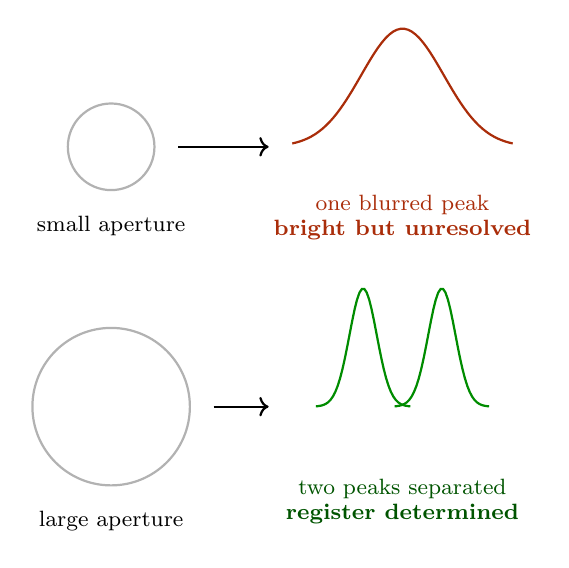
\begin{tikzpicture}[scale=1.0]
  % small aperture, long exposure
  \begin{scope}
    \draw[thick, gray!60] (0,0) circle (0.55);
    \node[below] at (0,-0.75) {\footnotesize small aperture};
    \draw[->, thick] (0.85,0) -- (2.0,0);
    \draw[thick, cruciblered] plot[domain=2.3:5.1, samples=60]
        ({\x}, {1.5*exp(-((\x-3.7)^2)/0.55)});
    
    \node[align=center, cruciblered] at (3.7,-0.9) {\footnotesize one blurred peak\\[-3pt]\footnotesize \textbf{bright but unresolved}};
  \end{scope}
  % large aperture
  \begin{scope}[yshift=-3.3cm]
    \draw[thick, gray!60] (0,0) circle (1.0);
    \node[below] at (0,-1.2) {\footnotesize large aperture};
    \draw[->, thick] (1.3,0) -- (2.0,0);
    \draw[thick, signalgreen] plot[domain=2.6:3.8, samples=40]
        ({\x}, {1.5*exp(-((\x-3.2)^2)/0.06)});
    \draw[thick, signalgreen] plot[domain=3.6:4.8, samples=40]
        ({\x}, {1.5*exp(-((\x-4.2)^2)/0.06)});
    \node[align=center, signalgreen!60!black] at (3.7,-1.2) {\footnotesize two peaks separated\\[-3pt]\footnotesize \textbf{register determined}};
  \end{scope}
\end{tikzpicture}
\caption{Aperture, not exposure. \texttt{s2\_stellar\_kinematics} carried 1{,}808{,}145 records
--- an enormous exposure --- across a span giving $M/N = 1.15$. A very large light bucket behind
a very small mirror. It could have detected something faint and could never have said where it
was.}
\end{figure}

\begin{signalbox}
\textbf{This is why \texttt{quantum\_transitional} is the domain that works.} NIST transitions
run from $4.8 \times 10^{6}$ to $4.9 \times 10^{16}$~Hz --- ten orders of magnitude, a log-span
of 23.04. Its 189{,}330 records are a modest exposure by this survey's standards. \emph{The
range is what does the work.}
\end{signalbox}

\begin{warningbox}
\textbf{Design rule for the rebuild: maximise orders of magnitude, not row count.} One hundred
thousand records spanning ten decades beats ten million spanning two. The like-for-like
requirement keeps it one population; the width is the aperture.
\end{warningbox}

\section{The Domains \texttt{log1p} Was Hiding}

There is a second reason so many domains piled below the lock floor, and it is the transform
rather than the data.

For $x \ll 1$, $\ln(1+x) \approx x$. The transform \emph{compresses} small values toward zero,
so a domain living entirely below unity has its dynamic range crushed before the statistic ever
sees it. Pure $\log$ is scale-free and does not.

\begin{table}[H]
\centering
\small
\begin{tabular}{@{}lrrl@{}}
\toprule
\textbf{Domain} & \textbf{periods under $\ln(1+x)$} & \textbf{periods under $\ln x$} & \\
\midrule
\texttt{stellar\_spindown} & \textbf{0.00} & \textbf{77.8} & recovered \\
\texttt{subnuclear\_eta} & 3.54 & 29.2 & recovered \\
\texttt{orbital\_eccentricity} & 1.93 & 19.8 & recovered \\
\texttt{orbital\_mass} & 3.15 & 15.0 & recovered \\
\texttt{galactic\_sersic} & 1.98 & 13.3 & recovered \\
\texttt{orbital\_radius} & 6.89 & 18.4 & improved \\
\texttt{quantum\_transitional} & 66.7 & 66.7 & unchanged \\
\texttt{t4\_cosmological} & 1.33 & 1.4 & \textbf{still thin} \\
\bottomrule
\end{tabular}
\caption{Periods spanned at $16/\pi$ under the two transforms.}
\end{table}

\texttt{stellar\_spindown} is the extreme case. Pulsar spin-down rates run from
$1.2\times10^{-21}$ to $5.5\times10^{-10}$~s/s --- eleven orders of magnitude of real physical
variation. Under $\ln(1+x)$ with $x_0 = 1$ the entire domain collapses to scalars of order
$10^{-10}$, nine orders beneath the lock floor, carrying \textbf{zero information}. Under
$\ln x$ it carries 77.8 periods.

\begin{nullbox}
The eleven orders of magnitude were always in the data. The transform was hiding them.

\medskip
\noindent \texttt{t4\_cosmological} is the honest exception. Its narrow redshift slice ---
$z \in [0.0100, 0.0160]$, a distance range of 42.8 to 68.4~Mpc --- spans 1.4 periods under
either transform. That is a genuine limit of the lake, not an artifact of the mathematics, and
no change of statistic repairs it.
\end{nullbox}

\section{Where the Recovery Comes From, and Why That Is a Risk}

The referee raised the objection that matters most here, and it is adopted as a condition rather
than answered.

For $x \gg 1$ the two transforms agree closely. The divergence is entirely at small $x$.
\textbf{Every recovered domain is recovered by expanding dynamic range at the low end --- which
is precisely where measurement error is largest, where detection limits bite, and where
non-physical records accumulate.}

We already know exactly what that looks like. \texttt{s2\_stellar\_kinematics} carries 497{,}831
records below $0.19$~km/s --- 27.5\% of the lake, against an expected $0.002\%$ for a stellar
population with $\sigma \approx 30$~km/s --- with a minimum of $4.88\times10^{-13}$~km/s. Under
the phase engine those records sat below the floor and were discarded. \textbf{Under the period
engine they are full participants, and they dominate the low-end range that generates the
resolution gain.}

\begin{rulingbox}
\textbf{No domain with sub-unit or near-detection-limit mass runs on the period engine until its
physical-validity floor is filed.}

\medskip
\noindent Not a lock floor --- a \emph{measurement-validity} floor, drawn from the instrument's
stated detection limit or the quantity's physical range, cited to an independent source, filed
before the run. For Gaia this is proper motion above a fixed multiple of its own quoted
uncertainty; a threshold chosen at the scalar level, after we know which side helps, is not
admissible.

\medskip
\noindent Every recovered domain publishes: records excluded by the floor, log-span and $M/N$
before and after, and the result both ways.
\end{rulingbox}

\section{The New Lake Boundaries}

The following become standing promotion requirements. They are the operational residue of the
entire crucible, and no lake is admitted without them.

\begin{enumerate}
    \item \textbf{Native precision.} A lake states the precision of its source and promotes at
          it. Rounding is a promotion decision and must be declared, not inherited. This is the
          Form E remedy.
    \item \textbf{Declared physical plausibility range.} Every lake states the expected range of
          its quantity from independent physics, and the fraction of records outside it, before
          admission. The distributional litmus test cannot see physical implausibility: a lake
          roughly a quarter composed of non-measurements passed it.
    \item \textbf{Measured object overlap.} Where two lakes may describe the same objects, the
          overlap is \emph{measured}, not assumed. Where partial, intersecting records are removed
          from one pre-registered side rather than a domain being discarded.
    \item \textbf{Declared dynamic range and $M/N$.} Log-span, and $M/N$ at every register the
          lake will be tested at, published before promotion. \textbf{A lake that cannot resolve
          the register it is being promoted to test is not promoted.}
    \item \textbf{Declared physical-validity floor}, from an independent source, for any lake
          with sub-unit or near-detection-limit mass.
    \item \textbf{Distinct-value count and grid detection}, including the $\log 2$ span test of
          Chapter 13.
\end{enumerate}

\subsection{A worked example of requirement 3}

\texttt{t4\_cosmological} (SDSS DR16 redshift) and \texttt{g1\_galaxy\_kinematics} (SDSS DR16
velocity dispersions) were candidates to be collapsed into one family on the suspicion of shared
objects. Rather than assume, the overlap was measured by sky-position match at
1-arcsecond tolerance:

\begin{table}[H]
\centering
\small
\begin{tabular}{@{}lr@{}}
\toprule
matched pairs & 971 \\
fraction of \texttt{t4\_cosmological} & 19.42\% \\
fraction of \texttt{g1\_galaxy\_kinematics} & 0.053\% \\
redshift range overlap & 100\% of A, 0.6\% of B \\
\bottomrule
\end{tabular}
\end{table}

Partial, not fatal. The 971 intersecting records are removed from \texttt{t4\_cosmological} and
both domains retained as independent families. Collapsing an entire domain on a suspicion would
have discarded a lake over a fifth of a small sample.

The measurement also surfaced its own caveat: \emph{zero} object overlap would not have implied
independence. Two disjoint samples drawn from the same flux-limited survey over the same
redshift range are correlated through selection \cite{malmquist1922}.

% ==============================================================================
\chapter{Pre-Registrations for the Period Engine}
% ==============================================================================

\section{Filed Before a Line of Code Exists}

Everything below was filed at Zenodo before any period-engine source file was written. The
fingerprint of the code that runs these trials is recorded against the filing.

Where a falsification condition exists, it is stated. Where the architect holds an expectation,
it is recorded --- including where that expectation is the outcome least favourable to the
framework, and including one prediction that was reversed on the basis of a measurement before
filing.

\begin{predictionbox}
\textbf{Statement of scope, stated here rather than discovered in a table.}

The period engine's resolution requirement --- $M/N > 2.67$ for a non-empty background annulus
--- is met by \textbf{one domain of nine} in the current survey. The architecture is filed on
the strength of its unit-invariance proof and its framework-agnostic data product, with the
explicit acknowledgement that its present coverage is one domain, and that \textbf{extending
that coverage requires lakes with greater dynamic range rather than improvements to the
statistic}.
\end{predictionbox}

\section{Trial 2b --- The Sector Bound Test}

\textbf{Run first, before all else.} It requires no engine, no annulus, no background, no null,
and no resolution margin.

Erratum 4a withdrew \texttt{stellar\_kinematic} on the diagnosis that a per-sector additive
offset, applied to the lake before the pipeline saw it, manufactured the $15/\pi$--$16/\pi$
band. That diagnosis has never been tested directly. The circular resultant makes it testable
by an inequality.

Decompose the total resultant by sector:

\begin{equation}
R_{\text{total}} \;=\; \left| \sum_j \frac{n_j}{n} R_j e^{i\Psi_j} \right|
\;\le\; \sum_j \frac{n_j}{n} R_j .
\label{eq:sectorbound}
\end{equation}

\begin{signalbox}
\textbf{A per-sector shift rotates each sector's resultant. It cannot lengthen it.}

\medskip
\noindent Therefore a sector shift \emph{cannot manufacture periodicity}. It can only align, or
fail to align, periodicity that each sector already possesses.
\end{signalbox}

\begin{predictionbox}
\textbf{Computed quantity 1 --- per-sector resultants $R_j$ on RAW values.}

\textbf{PREDICTION: every $R_j$ at chance level, $R_j \approx 1/\sqrt{n_j}$ within ordinary
fluctuation.}

\textbf{Failure mode:} any sector returning $R_j$ well above $1/\sqrt{n_j}$ means real
per-sector periodicity exists, the offsets merely aligned it, and \textbf{the Form C diagnosis
of Erratum 4 is wrong and must be rewritten.}

\medskip
\textbf{Computed quantity 2 --- the bound of Equation~\ref{eq:sectorbound}.} This is
algebraically guaranteed and is therefore \textbf{an implementation check, not a prediction}. If
the computed $R_{\text{total}}$ exceeds the bound, the code is wrong, not the physics.
\end{predictionbox}

\textbf{Form C is confirmed if every $R_j$ sits at chance; refuted if any sector carries genuine
periodicity.} This is the only test in the programme capable of proving our own diagnosis wrong,
and it is the number the referee most wants.

\section{Trial 1 --- \texttt{quantum\_transitional} --- the Build Gate}

\begin{predictionbox}
\textbf{PREDICT: $16/\pi$}, with a clear peak excess above background. $M/N = 4.17$, the highest
resolution margin in the survey.

\medskip
\textbf{Rationale.} Continuous support with more than 50{,}000 distinct values; field resolved at
top level, never fell to the legacy fallback in any engine version; zero records below the lock
floor at any register; immune to the $\log 2$ family; register unmoved across two independent
unseeded runs; and it strengthened at every tightening of the phase instrument,
$+28.5 \to +30.6 \to +31.2$.

\medskip
\textbf{If it fails:} either the $16/\pi$ result was unit-contingent after all, or the period
statistic is wrong. Both are decisive, both are reported, and \textbf{the build does not
proceed.}
\end{predictionbox}

\textbf{Subject to the Rydberg null of Chapter 13.} The requirement is not that the domain shows
a peak at $16/\pi$; it is that the real lake \emph{exceeds} the Rydberg null there.

\section{Trial 1b --- \texttt{orbital\_wrongbox} --- Clean Expected-Fail}

\begin{predictionbox}
\textbf{PREDICT: null} at every scoreable register.

\medskip
\textbf{Rationale.} The one demonstrated-clean control in the wrongbox tier: real data, a
genuinely wrong projection, cubed orbital periods spanning six orders of magnitude, no floor
mass, and $\Delta \approx 0$ under the phase engine. No confound attached.

\medskip
\textbf{A trial set that cannot demonstrate the instrument disagreeing proves nothing.}
\end{predictionbox}

\section{Trial 4 --- \texttt{stellar\_spindown} --- the Recovered Domain}

\begin{predictionbox}
\textbf{PREDICT: nothing. Register UNKNOWN.}

\medskip
\textbf{Rationale.} Zero information under $\ln(1+x)$; 77.8 periods under $\ln x$. No prior
exists and none will be invented. Any register it returns is reported as a first measurement
requiring independent confirmation, \textbf{never as a confirmation of anything}.

\medskip
\textbf{Conditional} on its physical-validity floor being filed before it runs.
\end{predictionbox}

\section{Trial 3 --- Struck}

\begin{warningbox}
No scoreable Form E domain exists. \texttt{planetary\_atlantic} sits at $M/N = 0.25$ and
\texttt{orbital\_ttv} at $1.32$ --- both below the annulus threshold.

\medskip
\noindent An earlier draft filed a prediction of ``excess below 5 at every resolvable
register'', which is \textbf{vacuously satisfied when no register is resolvable}. A prediction
that cannot fail is not a prediction, and this programme has already retired one gate for
exactly that defect.

\medskip
\noindent Rather than manufacture a domain to fill the slot, \textbf{the trial is struck and the
period engine's coverage gap on quantised support is named as unresolved.} Form E remains with
the phase engine's distinct-value and grid-spacing screens. If a high-dynamic-range quantised
domain is ever promoted, this test becomes available and will be taken.
\end{warningbox}

\section{The Comb Test}

\begin{predictionbox}
Run alongside Trial 1, on the same domain, since both are period scans and the marginal cost of
scanning continuously rather than at 23 points is small.

\textbf{Scan the period continuously over a range spanning several registers.}
\begin{itemize}
    \item Do the excess peaks fall on a comb of uniform spacing $\Delta_0$?
    \item Is $\Delta_0$ consistent with $\ln \kgeo / 24\pi = 0.0215902$?
\end{itemize}

\textbf{Residual ambiguity, stated before running:} a comb determines its fundamental only up to
integer subdivision. Even a clean result fixes $\ln \kgeo$ only up to a rational factor.
\end{predictionbox}

\section{The Comparison Matrix}

Pre-registered before either engine runs on any domain.

\begin{table}[H]
\centering
\small
\begin{tabular}{@{}lp{0.24\textwidth}p{0.24\textwidth}p{0.22\textwidth}@{}}
\toprule
& \textbf{period locks} & \textbf{period null} & \textbf{period unresolved} \\
\midrule
\textbf{phase locks} &
\cellcolor{signalgreen!12}\textbf{ROBUST} --- survives both formulations &
\cellcolor{goldseal!12}\textbf{PHASE-ONLY} --- suspect unit / floor / $x_0$ &
\cellcolor{gray!12}\textbf{UNDECIDABLE} --- data lacks the range \\
\textbf{phase null} &
\cellcolor{goldseal!12}\textbf{PERIOD-ONLY} --- split by the validity floor &
\cellcolor{gray!8}\textbf{NULL} &
\cellcolor{gray!12}\textbf{UNDECIDABLE} \\
\bottomrule
\end{tabular}
\end{table}

\begin{itemize}
    \item A \textbf{headline claim requires ROBUST.}
    \item \textbf{PERIOD-ONLY splits} by the physical-validity floor: re-run above the
          pre-registered floor. Excess survives $\Rightarrow$ genuine recovery, eligible for
          provisional reporting. Excess vanishes $\Rightarrow$ tail artifact, reported as such.
    \item \textbf{The third column is not a defect of either engine.} Three of the nine surviving
          domains land in it. Unresolved domains stay in the portrait with their $M/N$ printed;
          excluding them would hide the survey's own limits and would be selection on a quantity
          now known to correlate with register.
    \item The third column carries two labels: \textsc{resolution-limited} ($M/N < 1$, permanent)
          and \textsc{background-limited} ($1 < M/N < 2.67$, a to-do).
\end{itemize}

\begin{warningbox}
\textbf{Scope of ROBUST, which must be stated wherever the word is used.} The two engines share
the promoted lakes, the field mapping, the promotion decisions and the source data.

\medskip
\noindent \textbf{ROBUST means \emph{robust to the phase/period formulation}. It does not mean
independently confirmed.} Agreement between two engines reading a wrongly mapped field is the
same error twice, not corroboration.
\end{warningbox}

\section{Conditions of Adoption}

\begin{enumerate}
    \item Both engines run on every domain; both results published; never one.
    \item The comparison matrix above is pre-registered and not adjusted after results are seen.
    \item Recovered domains are pre-registered as \textbf{UNKNOWN}.
    \item \textbf{Physical-validity floors} filed per domain, from an independent source, before
          any recovered domain runs.
    \item The shared field mapping carries \textbf{runtime assertions}: each entry asserts that
          its path resolves and that its values match a recorded checksum, aborting on failure.
          Prose about a mapping is not a property of the mapping.
    \item The annulus parameters $1.6/M$ and $0.60/N$ and the sample count are \textbf{frozen at
          filing} and are not touchable after any real-data result is seen. Their fixture
          provenance and sensitivity table are published with them.
\end{enumerate}

\section{What Is Not Claimed}

The period formulation is not claimed correct and the phase formulation wrong. The phase engine
measures where on the grid structure sits, which would matter if the framework ever predicts a
phase.

Form C, Form B and same-object correlation are not removed by any statistic.

The five recovered domains are not results. They are domains that can now be \emph{measured},
subject to their validity floors --- a different and much smaller thing.

And the resolution criterion of Chapter 12 is not a discovery. It is textbook, it has been true
of every volume this programme has published, and we did not check it.

% ==============================================================================
\chapter{Standing, and the Road to Two Dimensions}
% ==============================================================================

\section{The Complete Taxonomy}

Volume 11 carried two artifact forms. Volume 12 carries five, plus two structural limits that
are not forms at all. The complete list is gathered here because it is the operational core of
everything the programme does from now on.

\begin{table}[H]
\centering
\small
\begin{tabular}{@{}clp{0.34\textwidth}p{0.24\textwidth}@{}}
\toprule
& \textbf{Form} & \textbf{Mechanism} & \textbf{Screen} \\
\midrule
A & Transform artifact &
The scalarization manufactures apparent structure from distribution shape alone &
Offset sweep; closed by theorem in 1D, \emph{not} extended to 2D \\
\addlinespace
B & Mundane concentration &
Real clustering from scale coincidence, selection, or ordinary physics --- demonstrated by the
Rydberg result &
Domain-specific physical nulls; open objection \\
\addlinespace
C & Preprocessing concentration &
Structure introduced by an operation applied to the lake before the pipeline saw it &
Dispatch attribution; the sector bound test \\
\addlinespace
D & Null-support mismatch &
The null's lockable support does not match the data's; a uniform null carries 2.5\% below-floor
mass where a skewed lake carries 27.5\% &
Common support; offset-sweep baseline; kept-fraction \\
\addlinespace
E & Quantised support &
Few distinct values, \emph{or} a span commensurate with the grid; the lock reduces to whether
those values land on nodes &
Distinct-value count; locked-mass concentration; $\log 2$ span test \\
\midrule
\multicolumn{4}{@{}l}{\emph{Structural limits --- properties of the data, not defects of the instrument}} \\
\midrule
--- & Resolution limit &
$M/N < 1$: the data cannot distinguish register $N$ from $N \pm 1$ &
$M/N$ published per domain per register \\
\addlinespace
--- & Degeneracy &
$N$ and $\ln \kgeo$ enter only as a product; the data determines a product, not a coordinate &
Comb test; theoretical derivation stated as such \\
\bottomrule
\end{tabular}
\caption{The complete taxonomy after Volume 12. Every screen runs on every domain on every run,
and its result is published whether or not it fires.}
\end{table}

\begin{signalbox}
\textbf{None of the five forms can manufacture a positive peak from nothing.}

\medskip
\noindent Form C displaces register assignment. Form D depresses every negative verdict and is
monotonic in $N$, so it cannot produce a local maximum. Form E inflates significance without
creating structure that is not present in the recorded values. The residual left by our own
correction is negative-signed at every register measured.

\medskip
\noindent \textbf{Every one of the twenty-eight \textsc{strong} domains in Volume 11 was scored
into a headwind.} The two structural limits are different in kind: they do not bias, they
\emph{deny}. They tell us which claims the data was never able to make.
\end{signalbox}

\section{What This Volume Costs and What It Buys}

\begin{table}[H]
\centering
\small
\begin{tabular}{@{}p{0.46\textwidth}p{0.46\textwidth}@{}}
\toprule
\textbf{Withdrawn, suspended, or restated} & \textbf{Established} \\
\midrule
\texttt{stellar\_kinematic} at $15/\pi$--$16/\pi$, carried since Volume 5 --- withdrawn &
Five artifact forms named, each with a screen that runs every time \\
\addlinespace
Four tidal domains, \texttt{orbital\_ttv}, \texttt{stellar\_cycle},
\texttt{galactic\_sersic} --- suspended pending native precision &
The resolution criterion: a limit that had governed every volume and was never measured \\
\addlinespace
Two of four wrongboxes --- demonstrating scale annihilation, not projection wrongness &
The degeneracy: what the data can and cannot determine about the modulus \\
\addlinespace
\texttt{stellar\_spindown} --- carried zero information under the old transform &
Unit invariance closed by proof rather than by inspection \\
\addlinespace
\texttt{n4\_cosmological} --- a null reproducing its own domain &
A framework-agnostic data product \\
\addlinespace
The \texttt{principle\_stellar\_proof} four-panel argument --- withdrawn pending rebuild &
The look-elsewhere correction adopted as an entry gate for every domain \\
\addlinespace
Bridge 1 --- register-unresolved from both ends &
Promotion standards: precision, plausibility, overlap, dynamic range, validity floors \\
\addlinespace
Falsification condition \#1 --- met on the published record, pending re-evaluation &
\textbf{Twenty-eight became nine, and nine became one that either engine can defend} \\
\bottomrule
\end{tabular}
\end{table}

\section{The One That Survived Everything}

\begin{signalbox}
\texttt{quantum\_transitional} --- 189{,}330 NIST atomic transitions.

\begin{itemize}
    \item \textbf{Continuous support}, more than 50{,}000 distinct scalar values. Form E cannot
          reach it, nor can the $\log 2$ commensurability family.
    \item \textbf{Field resolved at top level.} It never touched the legacy fallback in any
          engine version. Form C cannot reach it.
    \item \textbf{Zero records below the lock floor} at any of the 23 registers --- kept
          100--100\%. Form D cannot reach it.
    \item \textbf{Log-span 23.04, $M/N = 4.17$} --- the highest resolution margin in the survey,
          and the only domain above the annulus threshold.
    \item \textbf{Register stable} across two independent unseeded runs.
    \item \textbf{Global significance beyond $8\sigma$} after look-elsewhere correction across
          1{,}150 trials.
    \item It \textbf{strengthened at every tightening of the instrument}: $+28.5 \to +30.6 \to
          +31.2$.
\end{itemize}
\end{signalbox}

That last line is the one we would ask a sceptical reader to weigh. Every correction in this
volume cost the ledger claims. This domain gained from each of them.

\begin{warningbox}
And it is not yet safe. Chapter 13 shows that pure Rydberg structure --- $1/n^2$ and $Z^2$, no
lattice --- produces a register peak at $8/\pi$ with excess $+61.5$, and that
$\Delta_{16} = 2\Delta_8$ exactly, so $8/\pi$ structure produces $16/\pi$ power by harmonic
relation.

\medskip
\noindent \textbf{The Rydberg null gates every claim resting on this domain}, and it has not
been run. We state that here rather than after someone asks.
\end{warningbox}

\section{The Direction-of-Effect Audit}

If a finger were on the scale, corrections would increase results. Over five weeks of engine
work, ours did the opposite, systematically: $28 \to 21 \to 9 \to 1$ scoreable under the
stricter instrument. Five artifact forms found, every one biasing against the framework. Two
structural limits found, both narrowing what the survey may claim. One number moved up.

\begin{signalbox}
That is an auditable claim about \emph{direction of effect}, and it is the strongest evidence
available to us that the instrument is not being tuned toward a preferred answer.

\medskip
\noindent Three wrong hypotheses in the final session alone --- the referee's spike mechanism,
the architect's test fixture, the architect's threshold --- produced three real findings. That
ratio has held for five sessions. A process in which being wrong reliably produces information
is functioning as an instrument rather than as an advocacy exercise.
\end{signalbox}

\section{The Road to Two Dimensions}

Everything in this volume exists to make two-dimensional work possible. The standing
requirements, gathered:

\begin{enumerate}
    \item \textbf{Immutable from the 1D engines.} No shared code.
    \item \textbf{Form A re-derived in 2D} before any 2D lock is trusted. The theorem is a 1D
          result and does not automatically extend.
    \item \textbf{The scramble null wired in from the first commit.}
    \item \textbf{The resolution criterion built in, not discovered.} Both coordinates carry
          their own requirement and the joint requirement is at least as strict as the stricter
          of the two.
    \item \textbf{Synthetic calibration before real data.} Six lakes, expectations filed in
          advance, and at least one carrying a pre-registered \emph{expected fail}.
\end{enumerate}

\subsection{Why the scramble null becomes real}

Erratum 1 established that the scramble null is inert in one dimension: the lock statistic is
computed over the multiset of scalars and is order-independent, so shuffling cannot change it.
Real and scramble lock rates come out bit-identical.

In two dimensions each record carries two coordinates, and shuffling one against the other
destroys genuine joint structure while preserving both marginals exactly.

\begin{figure}[H]
\centering
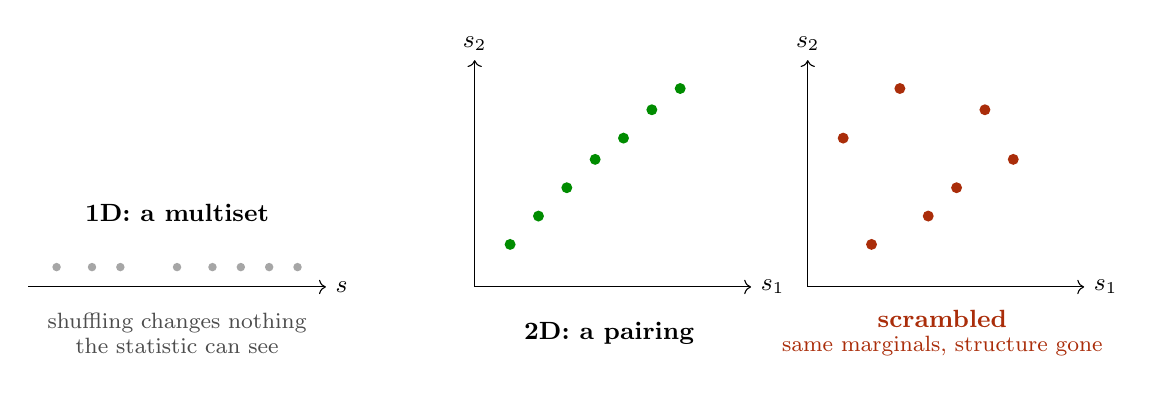
\begin{tikzpicture}[scale=0.9]
  \begin{scope}
    \draw[->] (0,0) -- (4.2,0) node[right] {\small $s$};
    \foreach \x in {0.4,0.9,1.3,2.1,2.6,3.0,3.4,3.8} \fill[gray!70] (\x,0.28) circle (1.7pt);
    \node at (2.1,1.05) {\small \textbf{1D: a multiset}};
    \node[align=center, gray!60!black] at (2.1,-0.65)
      {\footnotesize shuffling changes nothing\\[-3pt]\footnotesize the statistic can see};
  \end{scope}
  \begin{scope}[xshift=6.3cm]
    \draw[->] (0,0) -- (3.9,0) node[right] {\small $s_1$};
    \draw[->] (0,0) -- (0,3.2) node[above] {\small $s_2$};
    \foreach \p in {(0.5,0.6),(0.9,1.0),(1.3,1.4),(1.7,1.8),(2.1,2.1),(2.5,2.5),(2.9,2.8)}
      \fill[signalgreen] \p circle (2.2pt);
    \node at (1.9,-0.65) {\small \textbf{2D: a pairing}};
  \end{scope}
  \begin{scope}[xshift=11.0cm]
    \draw[->] (0,0) -- (3.9,0) node[right] {\small $s_1$};
    \draw[->] (0,0) -- (0,3.2) node[above] {\small $s_2$};
    \foreach \p in {(0.5,2.1),(0.9,0.6),(1.3,2.8),(1.7,1.0),(2.1,1.4),(2.5,2.5),(2.9,1.8)}
      \fill[cruciblered] \p circle (2.2pt);
    \node[align=center, cruciblered] at (1.9,-0.65)
      {\small \textbf{scrambled}\\[-3pt]\footnotesize same marginals, structure gone};
  \end{scope}
\end{tikzpicture}
\caption{In two dimensions each record carries two coordinates, and shuffling one against the other
destroys genuine joint structure while preserving both marginals exactly}
\end{figure}

\begin{predictionbox}
\textbf{The 2D calibration set.} The engine does not touch a real 2D lake until all six return
their pre-registered result.

\medskip
\begin{tabular}{@{}llp{0.40\textwidth}@{}}
\toprule
& \textbf{Construction} & \textbf{Pre-registered expectation} \\
\midrule
C1 & both coordinates uniform & null; $|z| < 3$ throughout \\
C2 & both log-normal, no harmonic relation & \textbf{null} --- the direct shape-artifact test \\
C3 & 30\% placed on a chosen register & strong lock at that register \emph{and nowhere else} \\
C4 & C3 with jitter at $1.5\times$ tolerance & degraded but detectable; calibrates sensitivity \\
C5 & C3 with one coordinate shuffled & \textbf{null} --- closes the loop Erratum 1 left open \\
C6 & C3 scaled below the lock floor & reports \textsc{out-of-range}, not null \\
\bottomrule
\end{tabular}

\medskip
\noindent The planted register is $19/\pi$, chosen deliberately away from $16/\pi$: planting at
the framework's own register and finding it would establish nothing we could trust about
ourselves. At least one lake carries a pre-registered \textbf{expected fail} --- a panel of six
passes proves the instrument agrees with itself, not that it can disagree.
\end{predictionbox}

\section{Closing: Optimistically Nervous}

The honest one-sentence summary of this volume is that we built an instrument, discovered it had
five ways of lying to us and two limits it had never measured, fixed what could be fixed, and
one domain was still standing at the end.

That is a shorter ledger than Volume 11 carried. It is also a better one, and the difference
between those two statements is the whole content of the crucible.

\begin{signalbox}
We want to be plain about the position, because a reader is entitled to it without having to
infer it.

\medskip
\noindent \textbf{The evidence today is one domain.} That is a lead, not a framework. The
cross-domain register agreement that Volumes 5 through 11 reported does not currently survive
the resolution criterion, and the bridge programme is in question until the domains are rebuilt
with fuller dynamic range. The falsification condition we ourselves filed appears to be met on
our own published record, and it will be reported either way.

\medskip
\noindent \textbf{And the one domain that survived, survived everything.} It is the only claim
in the programme that has faced every screen we could invent, and it grew stronger under each of
them. If it reproduces under a statistic that shares no scalarization, no null, no floor, no
$x_0$ and no unit convention with the first --- and if it exceeds the Rydberg null --- that will
be a stronger result than anything currently published here. Not a bigger number. A register
claim that is invariant \emph{by proof} rather than robust by inspection.
\end{signalbox}

The founder has described this as the hardest work the team has done, and it has taken longer
between publications than any interval in the programme's history. Both are true, and both were
the point. The work of this volume was not to add domains. It was to find out which of the ones
we had were entitled to be there, and to build the screens that will keep asking.

We are optimistic and we are nervous, and we think those are the correct proportions. The
signal, if it is there, will be there under a harder instrument. If it is not there, we would
rather find that ourselves, with the errata dated and the rulings published, than have it found
for us.

\begin{center}
\vspace{0.5em}
\itshape
Twenty-eight went into the fire. What comes out will have earned it.
\vspace{0.5em}
\end{center}


\appendix

% ==============================================================================
\chapter{Run Provenance}
% ==============================================================================

\section{Engine Fingerprints}

The engine fingerprint is the concatenated MD5 of the six files that fully determine pipeline
output. Every run in this volume is reproducible against its stated fingerprint.

\begin{table}[H]
\centering
\footnotesize
\begin{tabular}{@{}llp{0.34\textwidth}@{}}
\toprule
\textbf{Slot} & \textbf{File} & \textbf{Vol 12 canonical} \\
\midrule
$[0{:}32]$ & \texttt{engine/scalarize.py} & \texttt{044161a55b39c521e87f4c2bf4d7558f} \\
$[32{:}64]$ & \texttt{engine/unify.py} & \texttt{c78cb29cd07bf67abd2b4a5260366c03} \\
$[64{:}96]$ & \texttt{engine/build\_chaos\_nulls.py} & \texttt{d5d1612f9caf57d6b0c21459cc7e1a58} \\
$[96{:}128]$ & \texttt{engine/build\_pinch\_table.py} & \texttt{f103a7c433fe81b168f54dbcdeff6e49} \\
$[128{:}160]$ & \texttt{configs/scalarize.json} & run-specific \\
$[160{:}192]$ & \texttt{configs/volumes.json} & run-specific \\
\bottomrule
\end{tabular}
\end{table}

\section{The Audit Trail}

\begin{table}[H]
\centering
\footnotesize
\begin{tabular}{@{}lll@{}}
\toprule
\textbf{Run} & \textbf{Purpose} & \textbf{Outcome} \\
\midrule
\texttt{run\_20260816\_195207} & Two-anchor regression, Vol 11.1 statistic & Exposed the precomputed-scalar substitution \\
\texttt{run\_20260823\_003614} & First strict run & \textsc{aborted}: legacy fallback, six domain groups \\
\texttt{run\_20260823\_011734} & Full pipeline, clean field resolution & 28 \textsc{strong}, old statistic \\
\texttt{run\_20260826\_021811} & Corrected statistic, pinch only & Cross-domain matrix stale (checkpoint) \\
\texttt{run\_20260826\_025758} & \textbf{Canonical} & 21 \textsc{strong}; registers reproducible \\
\bottomrule
\end{tabular}
\end{table}

\section{Audit Scripts}

Released with this volume: \texttt{preflight\_audit.py}, \texttt{inspect\_schema.py},
\texttt{floor\_fraction\_s2.py}, \texttt{distinct\_value\_screen.py},
\texttt{validate\_common\_support.py}, \texttt{object\_overlap.py}, \texttt{ensemble\_z.py}.

Each is standalone and reproduces the corresponding figure or table in this volume from the
published lakes.

\clearpage

% ==============================================================================
\chapter*{References}
\addcontentsline{toc}{chapter}{References}
% ==============================================================================

\section*{The KishLattice Series}

All volumes are published open-access with full data, configuration, and engine
fingerprints. Every pre-registration listed below was filed prior to the run it governs.

\begin{itemize}
    \item Kish, T.~J. (2026). \textit{The Geometric Derivation of the Lattice} (Vol.~1).
          Zenodo. \url{https://doi.org/10.5281/zenodo.18209530}
    \item Kish, T.~J. et al.\ (2026). \textit{The Geometric Neutron} (Vol.~2).
          Zenodo. \url{https://doi.org/10.5281/zenodo.18217119}
    \item Kish, T.~J. et al.\ (2026). \textit{The Geometric Architecture of Matter} (Vol.~3).
          Zenodo. \url{https://doi.org/10.5281/zenodo.18217226}
    \item Kish, T.~J. et al.\ (2026). \textit{The Geometric Architecture of Life} (Vol.~4).
          Zenodo. \url{https://doi.org/10.5281/zenodo.18976975}
    \item Kish, T.~J. et al.\ (2026). \textit{The Geometric Architecture of Unification}
          (Vol.~5). Zenodo. \url{https://doi.org/10.5281/zenodo.19009634}
    \item Kish, T.~J. et al.\ (2026). \textit{The Harmonic Expansion of the Unified Lattice}
          (Vol.~6). Zenodo. \url{https://doi.org/10.5281/zenodo.19493376}
    \item Kish, T.~J. et al.\ (2026). \textit{The Sovereign Resonance: Boundaries,
          Sub-Lattice, and the Unification Case} (Vol.~7).
          Zenodo. \url{https://doi.org/10.5281/zenodo.19559860}
    \item Kish, T.~J. et al.\ (2026). \textit{Unbounded Luminosity: The Same-Object Harmonic
          Map and the Sovereign Lake Architecture} (Vol.~8).
          Zenodo. \url{https://doi.org/10.5281/zenodo.19622632}
    \item Kish, T.~J. et al.\ (2026). \textit{KishLattice Geometric Harmonic Spectroscopy:
          The First Survey of a New Field} (Vol.~9).
          Zenodo. \url{https://doi.org/10.5281/zenodo.19935603}
    \item Kish, T.~J. et al.\ (2026). \textit{The Deep Survey --- Seven New Domains and the
          Geometry of Life} (Vol.~10).
          Zenodo. \url{https://doi.org/10.5281/zenodo.20279208}
    \item Kish, T.~J. et al.\ (2026). \textit{The Structure That Locks --- The Spectroscopic
          Test and the Multi-Attribute Convergence} (Vol.~11).
          Zenodo. \url{https://doi.org/10.5281/zenodo.20587180}
\end{itemize}

\section*{Pre-Registrations and Supporting Papers}

\begin{itemize}
    \item Kish, T.~J. et al.\ (2026). \textit{Volume 9 --- Predictions Pre-Registration}.
          Zenodo. \url{https://doi.org/10.5281/zenodo.19702022}
    \item Kish, T.~J. et al.\ (2026). \textit{KishLattice Geometric Harmonic Spectroscopy:
          Volume 11 Pre-Registration (Multi-Attribute Sovereign Lake Expansion \&
          Dimensionality Falsification Protocol)}.
          Zenodo. \url{https://doi.org/10.5281/zenodo.20480506}
    \item Kish, T.~J. et al.\ (2026). \textit{Noise Does Not Lock --- A Comprehensive
          Empirical Response to Skeptical Challenges to KishLattice Geometric Harmonic
          Spectroscopy}. Zenodo. \url{https://doi.org/10.5281/zenodo.20585516}
          \\ \textit{Source of falsification condition \#1, formally re-evaluated in
          Chapter 13 of the present volume.}
    \item Kish, T.~J. et al.\ (2026). \textit{Master Equation of the Kish Lattice Theory ---
          The Rosetta Atlas}. Zenodo. \url{https://doi.org/10.5281/zenodo.18235735}
          \\ \textit{Subject of Erratum 6, Chapter 13.}
\end{itemize}

\section*{Repository and Project Resources}

\begin{itemize}
    \item Kish, T.~J. \textit{Holographic Resonance: The Geometry of a Quantized Universe} ---
          engine source, configurations, audit scripts and run receipts. GitHub.
          \url{https://github.com/TimothyKish/Holographic-Resonance-The-Geometry-of-a-Quantized-Universe}
    \item KishLattice 16$\pi$ Initiative LLC. \url{https://www.kishlattice.com}
\end{itemize}

\noindent The seven audit scripts released with this volume ---
\texttt{preflight\_audit.py}, \texttt{inspect\_schema.py}, \texttt{floor\_fraction\_s2.py},
\texttt{distinct\_value\_screen.py}, \texttt{validate\_common\_support.py},
\texttt{object\_overlap.py} and \texttt{ensemble\_z.py} --- are held in the repository above.
Each is standalone and reproduces the corresponding figure or table in this volume from the
published lakes.

\section*{Primary Data Sources --- Vol 12}

\begin{itemize}
    \item NIST Atomic Spectra Database (ASD), version 5.
          National Institute of Standards and Technology, Gaithersburg, MD.
          \url{https://physics.nist.gov/asd}
          \\ \textit{Source of} \texttt{quantum\_transitional}, \textit{the surviving anchor
          domain of this volume.}
    \item Gaia Collaboration (2022). Gaia DR3. VizieR catalog I/355.
          \\ \textit{Source of} \texttt{s1\_gaia\_parallax}, \texttt{s2\_stellar\_kinematics},
          \texttt{s3\_gaia\_luminosity}, \texttt{s4\_gaia\_colour}.
    \item Sloan Digital Sky Survey, Data Release 16. \url{https://www.sdss.org/dr16/}
          \\ \textit{Source of} \texttt{g1\_galaxy\_kinematics}, \texttt{galactic\_sersic},
          \texttt{galactic\_mass}, \texttt{t4\_cosmological}.
    \item CERN Open Data Portal (2014). CMS DoubleMu primary dataset, Run 2010B, Record 545.
          \url{https://opendata.cern.ch/record/545}
    \item NASA Exoplanet Archive. Confirmed planets and candidates (\texttt{pscomppars}).
          \url{https://exoplanetarchive.ipac.caltech.edu/}
    \item Holczer, T. et al.\ (2016). Transit Timing Observations from Kepler.
          \textit{ApJS}, 225, 9.
    \item Manchester, R.~N. et al.\ (2005). The Australia Telescope National Facility Pulsar
          Catalogue. \textit{AJ}, 129, 1993.
    \item McQuillan, A., Mazeh, T., \& Aigrain, S. (2014). Rotation periods of 34,030
          Kepler main-sequence stars. \textit{ApJS}, 211, 24.
    \item NOAA Center for Operational Oceanographic Products and Services (CO-OPS).
          High/Low tide predictions. \url{https://tidesandcurrents.noaa.gov/}
          \\ \textit{Source of the four tidal domains suspended under Form E, Chapter 4.}
    \item USGS Earthquake Hazards Program. FDSNWS event service.
          \url{https://earthquake.usgs.gov/fdsnws/event/1/}
    \item RCSB Protein Data Bank, and Richardson Lab Top8000 backbone validation dataset.
          \url{https://www.rcsb.org/}
    \item NNDC/IAEA. AME2020 atomic mass evaluation and NuDat nuclear data.
\end{itemize}

% ==============================================================================
\begin{thebibliography}{99}
\addcontentsline{toc}{section}{Scientific References}
\section*{Scientific References}

% --- Circular statistics and periodicity detection ---

\bibitem{rayleigh1879}
Rayleigh, Lord (J.~W. Strutt) (1879).
Investigations in optics, with special reference to the spectroscope.
\textit{Philosophical Magazine}, 8(49), 261--274.
\textit{(Origin of the resolution criterion applied in Chapter 12.)}

\bibitem{rayleigh1880}
Rayleigh, Lord (J.~W. Strutt) (1880).
On the resultant of a large number of vibrations of the same pitch and of arbitrary phase.
\textit{Philosophical Magazine}, 10(60), 73--78.
\textit{(Origin of the circular resultant statistic of Chapter 11.)}

\bibitem{mardia2000}
Mardia, K.~V., \& Jupp, P.~E. (2000).
\textit{Directional Statistics}. Wiley, Chichester.

\bibitem{fisher1993}
Fisher, N.~I. (1993).
\textit{Statistical Analysis of Circular Data}. Cambridge University Press.

\bibitem{bracewell2000}
Bracewell, R.~N. (2000).
\textit{The Fourier Transform and Its Applications} (3rd ed.). McGraw-Hill, Boston.
\textit{(Spectral leakage and the finite-aperture response used in Chapter 12.)}

\bibitem{gross2010}
Gross, E., \& Vitells, O. (2010).
Trial factors for the look elsewhere effect in high energy physics.
\textit{European Physical Journal C}, 70, 525--530.
\textit{(Basis of the look-elsewhere correction adopted in Chapter 1.)}

% --- Log-periodicity and discrete scale invariance ---

\bibitem{sornette1998}
Sornette, D. (1998).
Discrete scale invariance and complex dimensions.
\textit{Physics Reports}, 297(5), 239--270.
\textit{(The established literature on log-periodic structure with a physical mechanism.)}

\bibitem{sornette1996}
Sornette, D., \& Sammis, C.~G. (1995).
Complex critical exponents from renormalization group theory of earthquakes:
implications for earthquake predictions.
\textit{Journal de Physique I}, 5(5), 607--619.

\bibitem{johansen2000}
Johansen, A., Ledoit, O., \& Sornette, D. (2000).
Crashes as critical points.
\textit{International Journal of Theoretical and Applied Finance}, 3(2), 219--255.
\textit{(Cited as a cautionary case: log-periodic fitting criticised for arbitrary
fit windows and post-hoc period selection.)}

% --- Prior periodicity claims and their failure modes ---

\bibitem{tifft1976}
Tifft, W.~G. (1976).
Discrete states of redshift and galaxy dynamics I.
\textit{Astrophysical Journal}, 206, 38--56.
\textit{(The closest historical precedent to a cross-domain periodicity survey;
subsequently attributed to selection effects, limited dynamic range, and
reference-frame dependence.)}

\bibitem{napier1997}
Napier, W.~M., \& Guthrie, B.~N.~G. (1997).
Quantized redshifts: a status report.
\textit{Journal of Astrophysics and Astronomy}, 18, 455--463.

\bibitem{benford1938}
Benford, F. (1938).
The law of anomalous numbers.
\textit{Proceedings of the American Philosophical Society}, 78(4), 551--572.
\textit{(A statement about the distribution of fractional parts of $\log x$ in
heterogeneous natural data --- the same quantity the period statistic measures,
and the null any such claim must exceed.)}

\bibitem{hill1995}
Hill, T.~P. (1995).
A statistical derivation of the significant-digit law.
\textit{Statistical Science}, 10(4), 354--363.

% --- Atomic structure (the Form B null of Chapter 13) ---

\bibitem{rydberg1890}
Rydberg, J.~R. (1890).
Recherches sur la constitution des spectres d'\'emission des \'el\'ements chimiques.
\textit{Kongliga Svenska Vetenskaps-Akademiens Handlingar}, 23(11), 1--155.

\bibitem{bohr1913}
Bohr, N. (1913).
On the constitution of atoms and molecules.
\textit{Philosophical Magazine}, 26(151), 1--25.

\bibitem{nist_asd}
Kramida, A., Ralchenko, Yu., Reader, J., \& NIST ASD Team.
\textit{NIST Atomic Spectra Database} (version 5). National Institute of Standards
and Technology, Gaithersburg, MD. \url{https://physics.nist.gov/asd}

% --- Selection effects ---

\bibitem{malmquist1922}
Malmquist, K.~G. (1922).
On some relations in stellar statistics.
\textit{Meddelanden fran Lunds Astronomiska Observatorium}, Ser.~I, 100, 1--52.
\textit{(The selection mechanism by which two disjoint samples from one
flux-limited survey remain correlated --- Chapter 14, requirement 3.)}

% --- The controlled-experiment comparison of Chapter 1 ---

\bibitem{feynman1948}
Feynman, R.~P. (1948).
Space-time approach to non-relativistic quantum mechanics.
\textit{Reviews of Modern Physics}, 20(2), 367--387.

\bibitem{wen2026}
Wen, Y.-L., Tian, L.-M., Wang, Y., et al.\ (2026).
Direct experimental test of Feynman's path integral postulates with single photons.
\textit{Science Advances}, 12, eaeh1011.
\url{https://doi.org/10.1126/sciadv.aeh1011}
\textit{(South China Normal University. Probability amplitudes reconstructed for
more than $1.4$ million --- $17^5 = 1{,}419{,}857$ --- distinct optical paths.
Discussed in Chapter 1 as the controlled-experiment counterpart to archival survey work.)}

\bibitem{wen2026data}
Wen, Y.-L., Tian, L.-M., Wang, Y., et al.\ (2026).
\textit{Direct experimental test of Feynman's path integral postulates with single
photons} [Dataset]. Dryad.
\url{https://doi.org/10.5061/dryad.x0k6djj14}

\bibitem{scnu2023}
Wen, Y.-L., et al.\ (2023).
Demonstration of the quantum principle of least action with single photons.
arXiv:2305.19815 [quant-ph].
\url{https://arxiv.org/abs/2305.19815}
\textit{(Earlier propagator work by the same group, referenced in Chapter 1 as the
preceding fidelity benchmark.)}

\end{thebibliography}

% ==============================================================================
\section*{A Note on Citation Practice}
% ==============================================================================

Two conventions are followed throughout this volume and stated here so that a reader may
check them.

\textbf{Every empirical claim carries its run.} Where a number appears in this volume it is
traceable to a named run with a published engine fingerprint, or it is explicitly labelled as
a synthetic fixture, a reconstruction, or an expectation. Chapter 13 records an instance in
the Rosetta Atlas where this convention was not met --- five bullets of adjectives with no
table, no run reference and no fingerprint, two of which describe quantities no pipeline stage
computes --- and the passage is replaced with the Volume 5 three-target table and its actual
$z$-values.

\textbf{Prior art is cited even where it is unwelcome.} The quantized-redshift literature
\cite{tifft1976, napier1997} is the closest historical precedent to this programme and it
failed, for reasons --- selection effects, limited dynamic range, reference-frame dependence
--- that this volume has independently rediscovered as Forms B, the resolution criterion, and
Erratum 4f respectively. Benford's law \cite{benford1938, hill1995} is a statement about
precisely the quantity the period statistic measures and is the null any claim of this kind
must exceed. Discrete scale invariance \cite{sornette1998} is the established physics of
log-periodic structure, and it carries a mechanism where this framework does not yet.

We regard citing all three as a requirement rather than a courtesy. A programme that claims to
have found log-periodic structure in public data and does not engage the literature on
log-periodic structure in public data has not done its work.

% Guitar graphic - series ender
\begin{figure}[H]
\centering
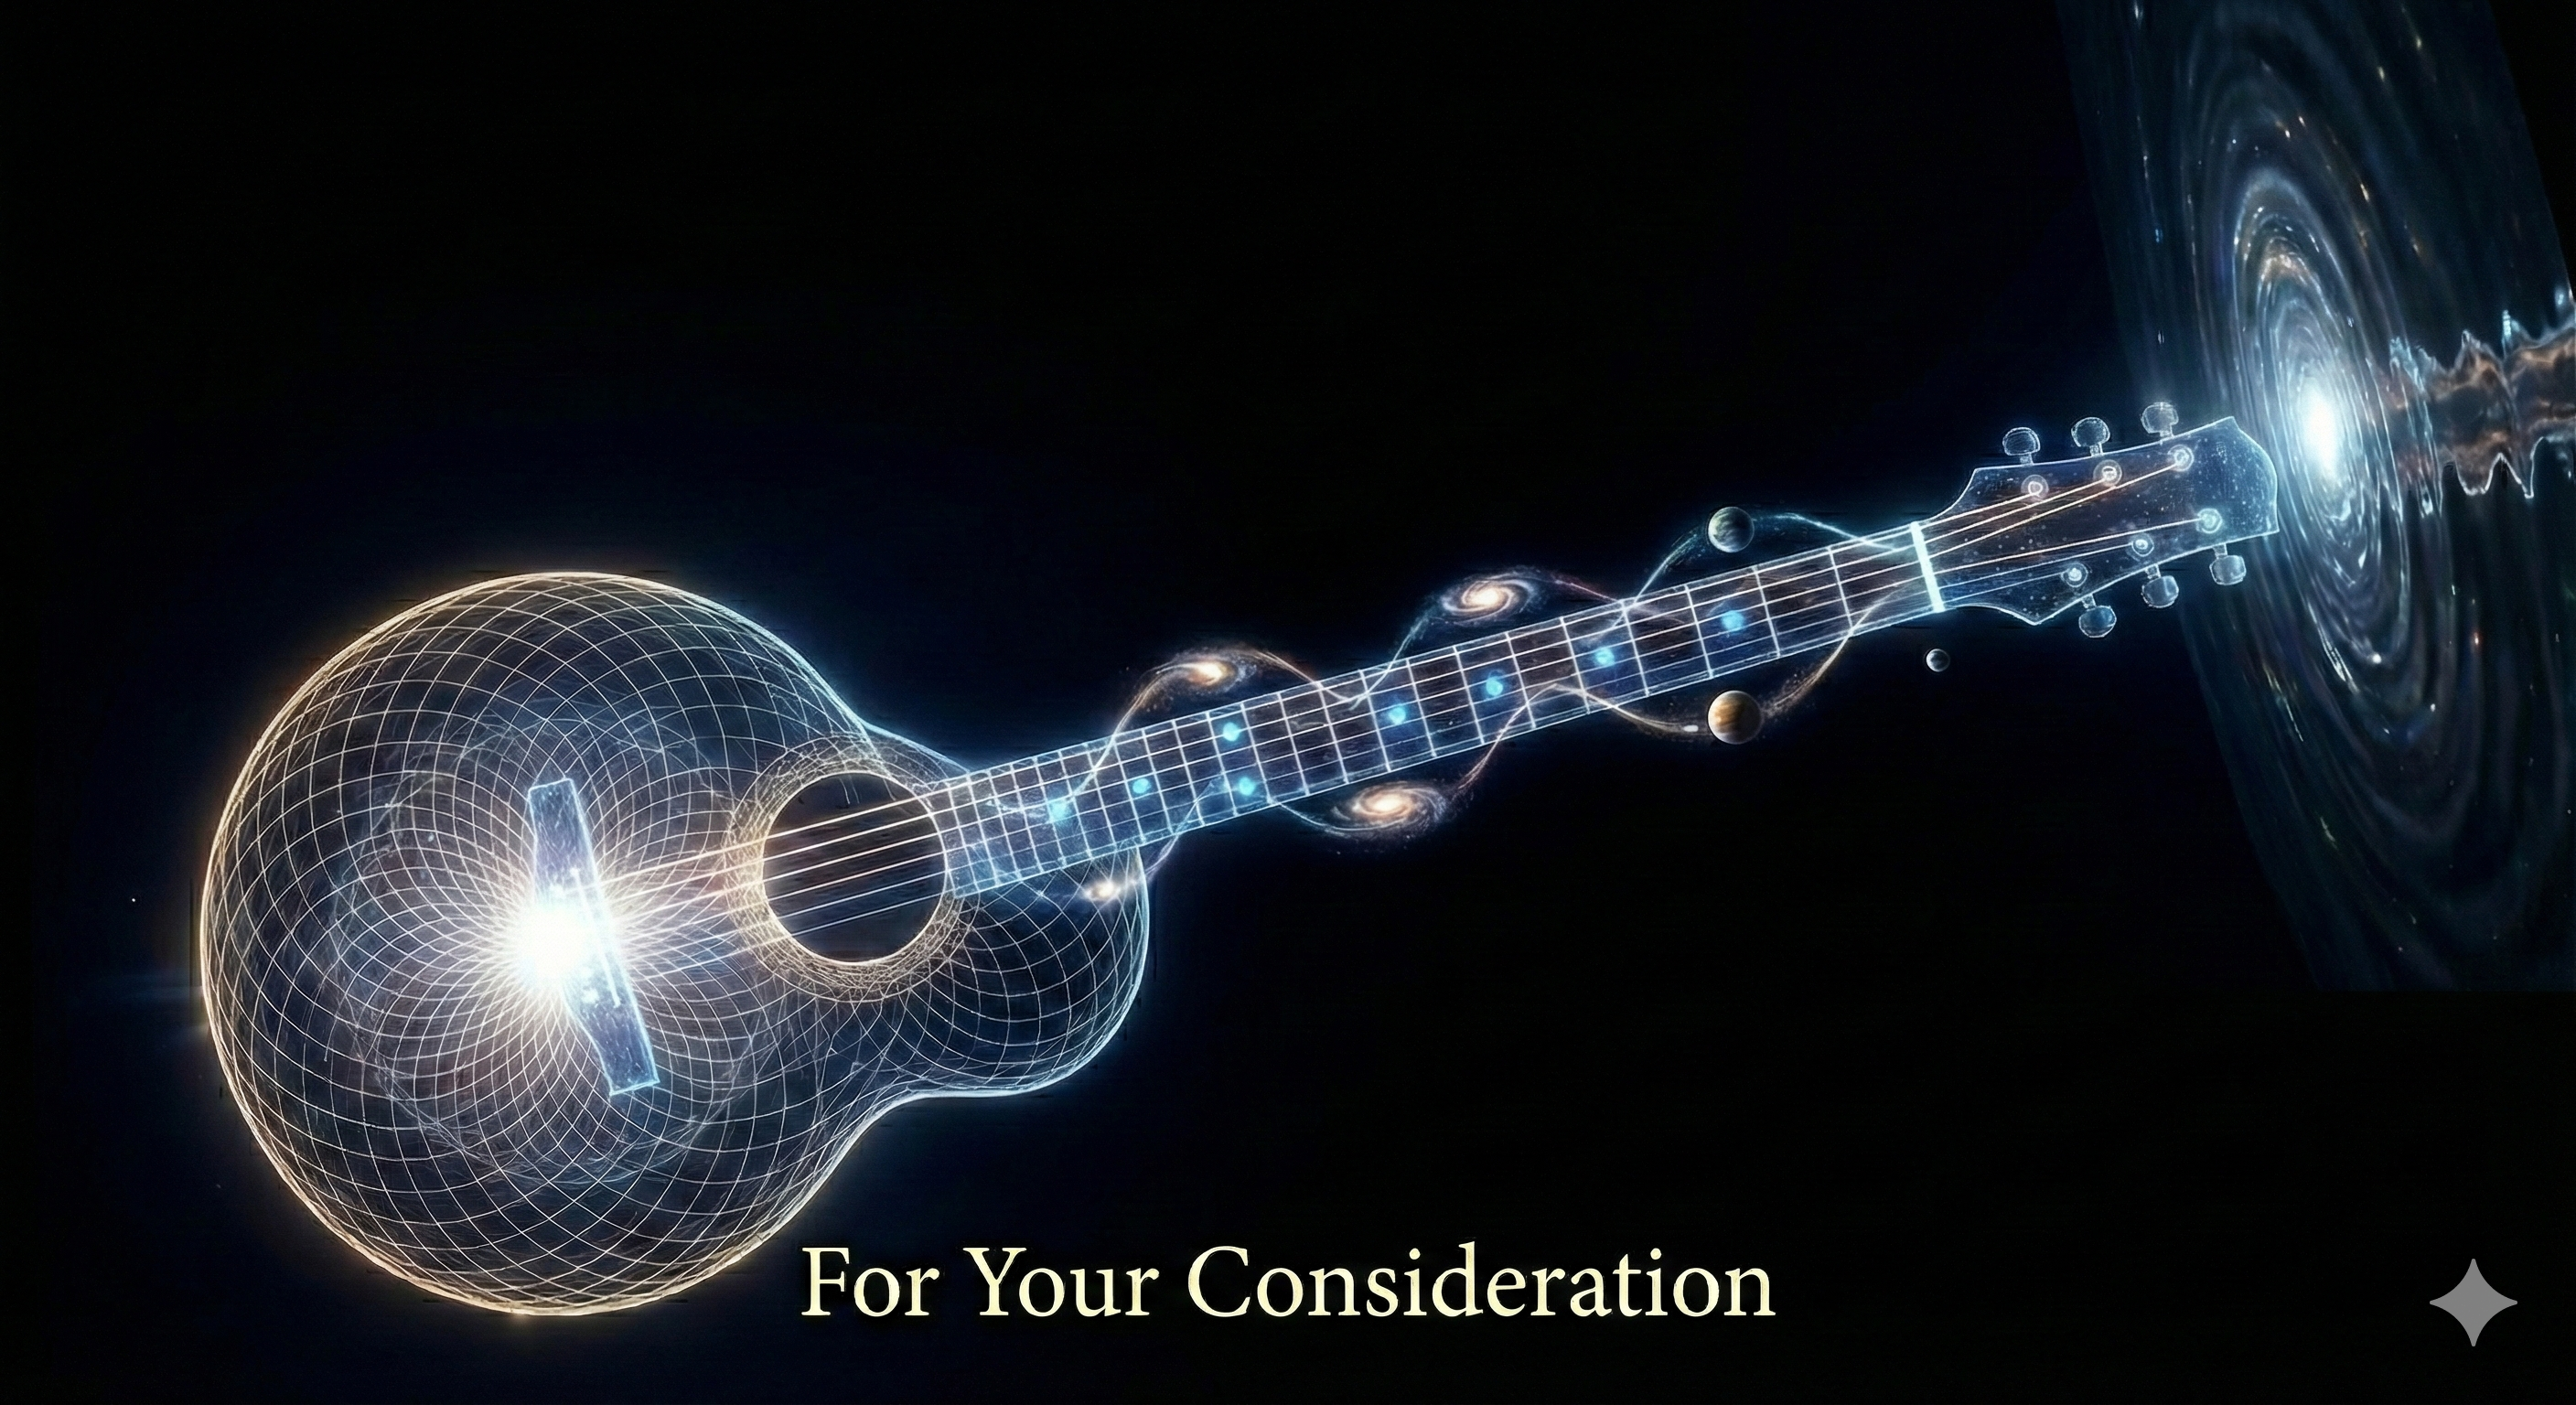
\includegraphics[width=0.85\textwidth]{Headers/ConclusionGuitar.png}
\end{figure}

\begin{center}
There is no Noise only Data. Remove the filters and see the Universe raw.
\end{center}

\end{document}
